% Define metadata
\documentclass{template/thesis}
\Title{ĐỀ TÀI: ỨNG DỤNG HỌC TĂNG CƯỜNG CHO CƠ CHẾ\\TỰ PHỤC HỒI TRONG CỤM KUBERNETES}
\Title[en]{TOPIC: APPLYING REINFORCEMENT LEARNING TO SELF-HEALING\\ IN KUBERNETES CLUSTERS}

\ThesisType{BÁO CÁO ĐỒ ÁN CHUYÊN NGÀNH}

\University{ĐẠI HỌC QUỐC GIA THÀNH PHỐ HỒ CHÍ MINH}
\CollegeOrDept{{TRƯỜNG ĐẠI HỌC CÔNG NGHỆ THÔNG TIN}}
\Faculty{KHOA MẠNG MÁY TÍNH VÀ TRUYỀN THÔNG}


\Author{NGUYỄN TIẾN PHÁT}{23521147}

\Degree{Môn học:}
\Major{NT114 - Đồ án chuyên ngành}
% \MajorCode{123}
\ThesisYear{2026}
\ThesisLocation{TP. HỒ CHÍ MINH}

\Supervisor{ThS. Lê Anh Tuấn}

\hypersetup{
	pdfencoding=auto,
	pdfauthor={Nguyễn Tiến Phát},
	pdfsubject={Môn học: NT114 - Đồ án chuyên ngành; Ngành: Mạng máy tính và truyền thông dữ liệu},
	pdftitle={Ứng dụng học tăng cường cho cơ chế tự phục hồi trong cụm Kubernetes},
	pdfkeywords={}
}

\usepackage{listings}
\lstset{
  basicstyle=\ttfamily\footnotesize,
  breaklines=true,
  backgroundcolor=\color{gray!5},
  frame=single,
  keywordstyle=\color{blue},
  commentstyle=\color{gray!60!black},
  stringstyle=\color{orange!80!black},
  numbers=none,
  tabsize=2,
  showstringspaces=false
}

\begin{document}
\firstbeforepreface
\secondbeforepreface
\afterpreface

\chapter{Giới thiệu}
\label{c:intro}
Chương mở đầu này cung cấp bối cảnh lý do chọn đề tài, 
xác định mục tiêu, đối tượng và phạm vi nghiên cứu, đồng thời 
trình bày cấu trúc tổng thể của đồ án. 
Đây là nền tảng để hiểu rõ ý nghĩa và định hướng của đồ án.
\section{Động cơ nghiên cứu}

Trong những năm gần đây, kiến trúc microservices và nền tảng container hóa đã trở thành xu hướng 
chủ đạo trong việc triển khai các hệ thống phân tán hiện đại. Kubernetes hiện là nền tảng 
điều phối phổ biến nhất, được sử dụng rộng rãi để quản lý container, tự động triển khai, mở rộng 
và vận hành hệ thống dịch vụ quy mô lớn. Một trong những đặc điểm quan trọng của Kubernetes là 
khả năng \textit{tự phục hồi} (self-healing), cho phép hệ thống tự động khởi động lại Pod lỗi, thay thế Pod bị crash hoặc điều phối workload sang Node khác khi xảy ra sự cố.

Tuy nhiên, cơ chế tự phục hồi mặc định của Kubernetes chủ yếu hoạt động dựa trên các rule cố định và các controller truyền thống. Trong các môi trường thực tế có tải động, số lượng dịch vụ lớn và lỗi xảy ra liên tục, các cơ chế này vẫn tồn tại nhiều hạn chế như:
\begin{itemize}
    \item Thời gian phục hồi chưa tối ưu.
    \item Không thích nghi tốt với nhiều loại lỗi đồng thời.
    \item Thiếu khả năng học hỏi từ dữ liệu lịch sử.
    \item Không tối ưu tài nguyên trong quá trình phục hồi.
\end{itemize}

Trong khi đó, Học tăng cường (Reinforcement Learning) là một nhánh của Học máy (Machine Learning) 
cho phép tác nhân (agent) học cách ra quyết định tối ưu thông qua quá trình tương tác với môi trường. 
Học tăng cường đã được ứng dụng trong nhiều bài toán tối ưu động như robot, mạng máy tính, quản lý 
tài nguyên đám mây và tối ưu lập lịch. Khả năng học chính sách tối ưu dựa trên trạng thái hệ thống 
giúp Học tăng cường trở thành hướng tiếp cận tiềm năng cho bài toán tự phục hồi trong Kubernetes.

Từ đó, đề tài “Ứng dụng Học tăng cường cho cơ chế tự phục hồi trong cụm Kubernetes” được thực hiện 
nhằm nghiên cứu khả năng áp dụng Học tăng cường để hỗ trợ ra quyết định phục hồi hệ thống hiệu quả 
hơn so với cơ chế mặc định.

\section{Mục tiêu đề tài}

Đề tài hướng đến các mục tiêu chính sau:
\begin{itemize}
    \item Nghiên cứu và phân tích các cơ chế tự phục hồi hiện tại của Kubernetes, đặc biệt trong 
    kịch bản Pod failure.
    \item Xây dựng môi trường ứng dụng microservices trên cụm Kubernetes. 
    \item Mô phỏng lượng người dùng và kịch bản lỗi thực tế.
    \item Thu thập dữ liệu trạng thái hệ thống thông qua các công cụ giám sát, phục vụ huấn luyện mô hình Học tăng cường.
    \item Thiết kế mô hình Học tăng cường hỗ trợ lựa chọn hành động phục hồi phù hợp.
    \item Đánh giá hiệu quả của mô hình sau huấn luyện dựa trên các tiêu chí như thời gian phục hồi, độ ổn định hệ thống 
    và khả năng thích nghi với lỗi.
\end{itemize}

\section{Phạm vi nghiên cứu}

Phạm vi nghiên cứu của đề tài tập trung vào bài toán tự phục hồi (self-healing)
trong môi trường Kubernetes thông qua việc ứng dụng học tăng cường nhằm hỗ trợ
quá trình ra quyết định phục hồi hệ thống khi xảy ra sự cố.

Nghiên cứu hướng đến việc xây dựng cơ chế phục hồi thông minh có khả năng
học từ dữ liệu vận hành của hệ thống để tối ưu hóa hiệu quả cứu hộ
trong môi trường microservices.

Đề tài được giới hạn trong kịch bản lỗi Pod CrashLoopBackOff. Đây là một
trong những sự cố phổ biến nhất, ảnh hưởng trực tiếp đến tính sẵn sàng
của hệ thống và thường gặp trong môi trường Kubernetes thực tế.

Môi trường thực nghiệm được xây dựng dưới dạng một cụm Kubernetes triển khai
ứng dụng microservices nhằm mô phỏng quá trình vận hành của hệ thống phân tán.

Dữ liệu được thu thập từ Kubernetes và các công cụ giám sát để xây dựng
tập dữ liệu huấn luyện cho bài toán Học tăng cường ngoại tuyến (Offline RL).

Tập dữ liệu bao gồm các thành phần cơ bản của mô hình như trạng thái hệ thống (state),
hành động phục hồi (action), phần thưởng (reward) và trạng thái kế tiếp (next state),
phản ánh rõ mối quan hệ giữa vận hành cụm và hiệu quả phục hồi.

Trong phạm vi nghiên cứu, nhóm dùng phương pháp huấn luyện dựa trên mô phỏng,
sau đó mới triển khai và đánh giá trên hệ thống thực nghiệm (Lab/Staging environment). 
Cách tiếp cận này giúp giảm nguy cơ gây mất ổn định và đảm bảo an toàn tuyệt đối
trước khi mô hình được xem xét cho các hệ thống thực tế.

Các hành động phục hồi được xem xét bao gồm: scale Pod, restart Pod,
reschedule workload, cordon hoặc drain Node, cũng như rollback dịch vụ khi xảy ra lỗi.

Hiệu quả của mô hình được đánh giá dựa trên thời gian phục hồi dịch vụ,
mức độ duy trì tính sẵn sàng, độ ổn định khi lỗi xảy ra liên tục
và khả năng thích nghi với nhiều trạng thái lỗi khác nhau.

Bên cạnh đó, đề tài không tập trung nghiên cứu các lĩnh vực ngoài bài toán tự phục hồi,
bao gồm: bảo mật và phát hiện tấn công, tối ưu autoscaling hoặc scheduling tổng quát,
điều phối đa cụm, cũng như triển khai trên môi trường production quy mô lớn.

Việc giới hạn này nhằm tập trung đánh giá sâu hiệu quả của Học tăng cường
đối với bài toán tự phục hồi trong Kubernetes một cách rõ ràng và nhất quán.

\section{Cấu trúc báo cáo}

Nội dung báo cáo được tổ chức thành bảy chương chính như sau:

\begin{itemize}
    \renewcommand{\labelitemi}{-}
    \item Chương 1: \textbf{Giới thiệu} -- Trình bày động cơ nghiên cứu, mục tiêu, phạm vi thực hiện và cấu trúc tổng thể của báo cáo.
    \item Chương 2: \textbf{Tổng quan lý thuyết, nghiên cứu liên quan} -- Tóm tắt các khái niệm nền tảng về Kubernetes, cơ chế self-healing, học tăng cường và các công trình liên quan đến tự phục hồi trong hệ thống cloud-native.
    \item Chương 3: \textbf{Mô hình bài toán} -- Mô tả bài toán self-healing dưới góc nhìn ra quyết định tuần tự, xây dựng mô hình MDP, không gian trạng thái, không gian hành động và hàm phần thưởng.
    \item Chương 4: \textbf{Phương pháp đề xuất} -- Trình bày kiến trúc phương pháp tiếp cận, quy trình thu thập dữ liệu, huấn luyện tác nhân RL và cách tích hợp mô hình vào bài toán tự phục hồi.
    \item Chương 5: \textbf{Cài đặt và thực nghiệm} -- Mô tả môi trường triển khai trên AWS, cụm k0s, hệ thống mini-ecommerce, công cụ giám sát, kịch bản tạo lỗi và cách triển khai tác nhân RL trên Kubernetes.
    \item Chương 6: \textbf{Kết quả và phân tích} -- Trình bày kết quả huấn luyện, kết quả đánh giá các chính sách, so sánh giữa các mô hình và phân tích tác động của cơ chế self-healing đến các chỉ số hệ thống.
    \item Chương 7: \textbf{Kết luận và hướng phát triển} -- Tóm tắt các kết quả đạt được, nêu ra hạn chế còn tồn tại và đề xuất các hướng mở rộng trong tương lai.
\end{itemize}



\chapter{Tổng quan lý thuyết, nghiên cứu liên quan}
\label{c:cosolythuyet}
\section{Tổng quan lý thuyết}

\noindent Chương này trình bày các nền tảng lý thuyết được sử dụng trong đề tài, bao gồm mô hình học tăng cường, tiến trình quyết định Markov và các thuật toán điều khiển chính sách/giá trị liên quan.

\section{Thuật toán DQN trong học tăng cường}

\noindent Deep Q-Network (DQN) là phương pháp học tăng cường theo giá trị (\textit{dựa trên giá trị}), trong đó tác nhân học hàm giá trị hành động $Q(s, a)$ để ước lượng mức lợi ích kỳ vọng khi chọn hành động $a$ tại trạng thái $s$.

\noindent\textbf{Mục tiêu tối ưu.}

\noindent Với hệ số chiết khấu $\gamma$, mục tiêu của DQN là cực đại hóa tổng phần thưởng tích lũy chiết khấu:
\[
G_t = \sum_{k=0}^{\infty}\gamma^k r_{t+k}
\]
Tác nhân lựa chọn hành động theo chính sách tham lam trên hàm Q:
\[
\pi(s) = \arg\max_{a} Q(s, a)
\]

\noindent\textbf{Xấp xỉ hàm Q bằng mạng neural.}

\noindent Thay vì lưu bảng Q truyền thống (khó mở rộng khi không gian trạng thái lớn), DQN sử dụng mạng neural tham số $\theta$ để xấp xỉ:
\[
Q(s, a; \theta)
\]
Đầu vào là vector trạng thái hệ thống (các đặc trưng từ MDP), đầu ra là giá trị Q tương ứng cho từng hành động rời rạc trong không gian hành động.

\noindent\textbf{Hàm mục tiêu Bellman và hàm mất mát.}

\noindent Tại mỗi bước cập nhật, mục tiêu Bellman được xây dựng:
\[
y = r + \gamma \max_{a'} Q_{\theta^-}(s', a')
\]
trong đó $\theta^-$ là tham số của \textit{mạng mục tiêu}. Hàm mất mát bình phương sai số:
\[
\mathcal{L}(\theta) = \mathbb{E}_{(s,a,r,s') \sim \mathcal{D}}
\left[
\left(y - Q_{\theta}(s,a)\right)^2
\right]
\]
với $\mathcal{D}$ là bộ nhớ kinh nghiệm (\textit{bộ nhớ kinh nghiệm}).

\noindent\textbf{Kỹ thuật ổn định huấn luyện.}

\begin{itemize}
    \item \textbf{Phát lại kinh nghiệm}: lưu các mẫu chuyển trạng thái $(s,a,r,s')$ và lấy mẫu ngẫu nhiên theo mini-batch để giảm tương quan theo thời gian giữa các mẫu huấn luyện.
    \item \textbf{Mạng mục tiêu}: sử dụng mạng mục tiêu với tham số $\theta^-$, được cập nhật định kỳ từ mạng chính $\theta$, giúp giảm dao động trong quá trình học.
    \item \textbf{Khám phá epsilon-greedy}: tại bước huấn luyện, với xác suất $\epsilon$ tác nhân chọn hành động ngẫu nhiên để khám phá; ngược lại chọn hành động có Q lớn nhất để khai thác.
\end{itemize}

\section{Nghiên cứu liên quan}

\noindent Phần này tổng hợp các công trình liên quan đến tự phục hồi hệ thống, tối ưu điều khiển trên Kubernetes và ứng dụng học tăng cường trong vận hành hệ thống phân tán.



\chapter{Mô hình bài toán}
\label{c:mohinhbaitoan}
\input{chapters/3-MoHinhBaiToan}

\chapter{Phương pháp đề xuất}
\label{c:phuongphapdexuat}
\section{Thiết kế hệ thống bằng UML (Unified Modeling Language)}

\noindent UML được sử dụng để mô tả kiến trúc và luồng xử lý của hệ thống tự phục hồi dựa trên RL theo cách trực quan, nhất quán giữa góc nhìn nghiên cứu và triển khai thực tế. Trong phạm vi đồ án, phần UML tập trung vào ba khía cạnh: chức năng hệ thống, trình tự tương tác khi xảy ra sự cố và cấu trúc triển khai các thành phần thời gian chạy.

\begin{figure}[!htbp]
\centering
\footnotesize
\begin{tikzpicture}[
    scale=0.90, transform shape,
    >=stealth,
    proc/.style={draw=blue!50, fill=blue!8, rounded corners=2mm, align=center, minimum width=9.2cm, minimum height=9mm},
    act/.style={draw=green!50!black, fill=green!8, rounded corners=2mm, align=center, text width=8cm, minimum height=9mm},
    noact/.style={draw=red!60, fill=red!6, rounded corners=2mm, align=center, minimum width=5.3cm, minimum height=9mm},
    dec/.style={draw=orange!70!black, fill=yellow!10, rounded corners=1.8mm, align=center, minimum width=5.8cm, minimum height=10mm},
    merge/.style={draw=violet!70!black, fill=violet!10, circle, inner sep=1.2pt},
    line/.style={->, thick}
]

\node (start) [circle, draw, fill=black, inner sep=1.7pt] {};
\node (collect) [proc, at={($(start)+(0,-1.15)$)}] {Thu thập số liệu từ Prometheus \& Kubernetes API};
\node (prep) [proc, at={($(collect)+(0,-1.35)$)}] {Tiền xử lý số liệu (Chuẩn hóa, Lọc nhiễu)};
\node (state) [proc, at={($(prep)+(0,-1.35)$)}] {Tạo biểu diễn trạng thái $s_t$};
\node (choose) [dec, at={($(state)+(0,-1.50)$)}] {Tác nhân RL chọn hành động \\ (DQN / A2C / PPO)};

\node (act1) [act, at={($(choose)+(-4.25,-1.75)$)}] {Hành động = Khởi động lại / Mở rộng / Thu hẹp / Không hành động};
\node (act2) [act, at={($(act1)+(0,-1.35)$)}] {Gửi hành động tới bộ chấp hành};
\node (act3) [act, at={($(act2)+(0,-1.35)$)}] {Bộ chấp hành thực thi lệnh an toàn trên Kubernetes};

\node (noaction) [noact, at={($(choose)+(3.35,-1.75)$)}] {Không thực hiện hành động};
\node (join) [merge, at={($(act3)+(4.25,-1.25)$)}] {};

\node (observe) [proc, at={($(join)+(0,-1.40)$)}] {Quan sát trạng thái kế tiếp $s_{t+1}$ và nhận thưởng $R_t$ \\ (Giảm MTTR, Tuân thủ SLO)};
\node (update) [proc, anchor=north, at={($(observe.south)+(0,-0.35)$)}] {Cập nhật mô hình RL \\ (DQN: mạng Q, A2C/PPO: mạng chính sách và giá trị)};
\node (store) [proc, anchor=north, at={($(update.south)+(0,-0.35)$)}] {Lưu chuyển trạng thái $(s_t, a_t, R_t, s_{t+1})$ phục vụ huấn luyện};
\node (cont) [proc, anchor=north, at={($(store.south)+(0,-0.35)$)}] {Tiếp tục giám sát và thích nghi};
\node (running) [dec, anchor=north, at={($(cont.south)+(0,-0.35)$)}] {Hệ thống còn hoạt động?};
\node (end) [circle, draw, fill=black, inner sep=1.7pt, at={($(running)+(0,-1.15)$)}] {};

\draw[line] (start) -- (collect);
\draw[line] (collect) -- (prep);
\draw[line] (prep) -- (state);
\draw[line] (state) -- (choose);

\draw[line] (choose.west) -| (act1.north);
\draw[line] (choose.east) -| (noaction.north);
\node[font=\bfseries\color{green!50!black}] at ($(choose.west)+(-2.0,-0.08)$) {Có};
\node[font=\bfseries\color{red!70!black}] at ($(choose.east)+(1.6,-0.08)$) {Không};

\draw[line] (act1) -- (act2);
\draw[line] (act2) -- (act3);

\draw[line] (noaction.south) |- (join.east);
\draw[line] (act3.south) |- (join.west);

\draw[line] (join) -- (observe);
\draw[line] (observe) -- (update);
\draw[line] (update) -- (store);
\draw[line] (store) -- (cont);
\draw[line] (cont) -- (running);
\draw[line] (running) -- node[midway, right] {\color{red!70!black}\textbf{Không}} (end);
\draw[line] (running.west) -| ++(-6.10,0) |- node[pos=0.25, left] {\color{green!50!black}\textbf{Có}} (collect.west);

\end{tikzpicture}
\caption{Luồng hoạt động cho vòng lặp tự phục hồi dựa trên RL}
\label{fig:rl-self-healing-activity}
\end{figure}
\clearpage

\section{Kế thừa MDP từ Chương 3 vào ba thuật toán}

\noindent Chương này không lặp lại định nghĩa MDP. Thay vào đó, nội dung tập trung vào cách \textbf{ánh xạ trực tiếp} các thành phần MDP ở Chương 3 vào ba thuật toán được sử dụng trong đồ án gồm DQN, A2C và PPO. Ba thuật toán cùng dùng chung một mô hình bài toán, khác nhau chủ yếu ở cơ chế học và cách cập nhật tham số.

\subsection{Ánh xạ trạng thái sang đầu vào mô hình}

\noindent Vector trạng thái $s_t$ gồm nhóm \textit{core state}, \textit{derived state} và \textit{extended state} nếu có, được chuẩn hóa theo đúng quy tắc ở Chương 3 trước khi đưa vào mô hình. Với DQN, $s_t$ là đầu vào của mạng Q để ước lượng $Q(s_t,a)$. Với A2C và PPO, $s_t$ đồng thời là đầu vào cho nhánh chính sách và nhánh giá trị.

\subsection{Ánh xạ hành động sang actuator và guardrail}

\noindent Không gian hành động rời rạc \{\texttt{idle}, \texttt{restart\_pod}, \texttt{scale\_up}, \texttt{scale\_down}\} được ánh xạ sang lệnh vận hành trên Kubernetes thông qua lớp actuator. Trước khi thực thi, mỗi hành động phải đi qua guardrail như thời gian chờ giữa hai hành động, giới hạn \textit{min/max replicas} và chế độ chạy thử, nhằm bảo đảm an toàn vận hành.

\subsection{Ánh xạ hàm thưởng sang mục tiêu huấn luyện}

\noindent Hàm thưởng thiết kế ở Chương 3 được dùng nguyên vẹn để sinh tín hiệu học tại mỗi bước. Với DQN, phần thưởng $R_t$ đi vào mục tiêu Bellman để cập nhật mạng Q. Với A2C và PPO, $R_t$ được dùng để tính return và advantage, từ đó tối ưu chính sách can thiệp và hàm giá trị trạng thái.

\subsection{Ánh xạ điều kiện kết thúc sang vòng lặp huấn luyện}

\noindent Ba điều kiện kết thúc gồm thành công, thất bại và hết thời gian được dùng làm tín hiệu đóng tập trong cả hai pha: thu thập rollout và huấn luyện theo tập. Nhờ vậy, dữ liệu huấn luyện phản ánh đúng các quỹ đạo phục hồi hợp lệ và giúp so sánh ba thuật toán trên cùng một tiêu chí dừng.

\section{Thuật toán DQN}

\noindent \textbf{Cơ sở lựa chọn thuật toán.}

\noindent Deep Q-Network (DQN) là phương pháp học tăng cường theo giá trị, học hàm $Q(s,a)$ để ước lượng lợi ích kỳ vọng của từng hành động tại mỗi trạng thái. Trong bài toán tự phục hồi Kubernetes, DQN phù hợp vì không gian hành động là rời rạc, nhỏ và rõ ràng, gồm bốn hành động phục hồi cơ bản.

\noindent Với tập hành động nhỏ như vậy, DQN thuận lợi cho việc xây dựng baseline nhanh, dễ theo dõi Q-value và thuận tiện gỡ lỗi hành vi chính sách. Trong phạm vi đồ án, DQN đóng vai trò là mô hình theo hướng \textit{value-based} để so sánh với các mô hình \textit{actor-critic} ở các phần sau.

\subsection{Thiết kế phương pháp cho kịch bản Pod Failure}

\subsubsection{Mục tiêu thiết kế}

\noindent Mục tiêu của DQN trong kịch bản Pod Failure là học chính sách ra quyết định phục hồi theo trạng thái hệ thống tại từng thời điểm. Chính sách cần phản ứng đủ nhanh khi chất lượng dịch vụ suy giảm, đồng thời tránh can thiệp dư thừa khi hệ thống đã quay về trạng thái ổn định.

\subsubsection{Ánh xạ trạng thái sang đầu vào mạng Q}

\noindent Trạng thái đầu vào kế thừa trực tiếp từ MDP ở Chương 3, gồm các đặc trưng phản ánh lưu lượng, lỗi, độ trễ và ngữ cảnh pha thí nghiệm. Trước khi đưa vào mạng Q, các đặc trưng được chuẩn hóa theo cùng quy tắc tiền xử lý đã định nghĩa trong mô hình bài toán để bảo đảm tính nhất quán giữa pha huấn luyện và pha suy luận.

\begin{center}
\begin{tikzpicture}[
    >=stealth,
    font=\small,
    line/.style={->, thick},
    box/.style={draw=blue!50, fill=blue!8, rounded corners=2mm, align=center, minimum width=12.4cm, minimum height=8.5mm, inner xsep=3mm}
]
\def\vsep{0.48}

\node (raw)   [box] at (0,0) {Số liệu thô từ hệ thống thực\\(CSV, Prometheus, Kubernetes API)};
\node (prep)  [box, anchor=north] at ($(raw.south)+(0,-\vsep)$) {Tiền xử lý dữ liệu\\(làm sạch, chuẩn hóa, clip)};
\node (feat)  [box, anchor=north] at ($(prep.south)+(0,-\vsep)$) {Tạo đặc trưng trạng thái\\(core state, derived state, extended state)};
\node (state) [box, anchor=north] at ($(feat.south)+(0,-\vsep)$) {Ghép vector trạng thái $s_t$};
\node (qnet)  [box, anchor=north] at ($(state.south)+(0,-\vsep)$) {Đầu vào mạng Q (DQN)};
\node (qval)  [box, anchor=north] at ($(qnet.south)+(0,-\vsep)$) {Đầu ra giá trị hành động\\$Q(s_t, a_0),\ Q(s_t, a_1),\ Q(s_t, a_2),\ Q(s_t, a_3)$};

\draw[line] (raw) -- (prep);
\draw[line] (prep) -- (feat);
\draw[line] (feat) -- (state);
\draw[line] (state) -- (qnet);
\draw[line] (qnet) -- (qval);

\end{tikzpicture}
\captionof{figure}{Luồng ánh xạ trạng thái sang đầu vào mạng Q trong DQN}
\label{fig:dqn-state-to-q-input}
\end{center}

\subsubsection{Ánh xạ hành động sang cơ chế can thiệp}

\noindent Đầu ra của DQN là giá trị Q ứng với từng hành động rời rạc. Hành động được chọn sẽ được ánh xạ sang lệnh can thiệp trên Kubernetes thông qua lớp actuator, bảo đảm mỗi quyết định của tác nhân đều có đường đi thực thi rõ ràng từ mức mô hình đến mức hệ thống.

\begin{center}
\begin{tikzpicture}[
    >=stealth,
    font=\small,
    line/.style={->, thick},
    box/.style={draw=blue!50, fill=blue!8, rounded corners=2mm, align=center, minimum width=12.0cm, minimum height=8.5mm, inner xsep=3mm},
    guard/.style={draw=orange!70!black, fill=yellow!10, rounded corners=2mm, align=center, minimum width=12.0cm, minimum height=8.5mm, inner xsep=3mm},
    act/.style={draw=green!50!black, fill=green!8, rounded corners=2mm, align=center, minimum width=12.0cm, minimum height=8.5mm, inner xsep=3mm}
]
\def\vsep{0.42}

\node (qout) [box] at (0,0) {Đầu ra mạng Q: chọn hành động có giá trị Q lớn nhất};
\node (map) [box, anchor=north] at ($(qout.south)+(0,-\vsep)$) {Ánh xạ hành động rời rạc sang lệnh Kubernetes};
\node (guard) [guard, anchor=north] at ($(map.south)+(0,-\vsep)$) {Guardrail: cooldown, giới hạn min/max replicas, chế độ chạy thử};
\node (exec) [act, anchor=north] at ($(guard.south)+(0,-\vsep)$) {Actuator thực thi lệnh an toàn lên cụm Kubernetes};
\node (fb) [box, anchor=north] at ($(exec.south)+(0,-\vsep)$) {Thu phản hồi hệ thống và ghi log hành động cho bước học tiếp theo};

\draw[line] (qout) -- (map);
\draw[line] (map) -- (guard);
\draw[line] (guard) -- (exec);
\draw[line] (exec) -- (fb);
\end{tikzpicture}
\captionof{figure}{Luồng ánh xạ hành động DQN sang cơ chế can thiệp và guardrail}
\label{fig:dqn-action-to-actuator}
\end{center}

\subsubsection{Cơ chế học và cập nhật tham số DQN}

\noindent DQN cập nhật giá trị hành động dựa trên phương trình Bellman, kết hợp \textit{replay buffer} và \textit{target network} để tăng ổn định. Chính sách lựa chọn hành động theo chiến lược \textit{epsilon-greedy}, trong đó tác nhân khám phá mạnh ở giai đoạn đầu và giảm dần mức khám phá khi quá trình học tiến triển.

\subsubsection{Ràng buộc an toàn khi thực thi}

\noindent Trước khi thực thi hành động, hệ thống áp dụng lớp guardrail để giảm rủi ro vận hành, bao gồm giới hạn tần suất can thiệp, giới hạn biên scale và chế độ chạy thử. Nhờ đó, chính sách học được vẫn nằm trong miền hành động an toàn khi chuyển sang môi trường runtime.

\subsubsection{Quy trình huấn luyện và đánh giá ở mức phương pháp}

\noindent Quy trình tổng quát gồm các bước: thu thập chuyển trạng thái, cập nhật mạng Q theo mini-batch, đồng bộ mạng mục tiêu theo chu kỳ và đánh giá định kỳ để chọn checkpoint. Việc đánh giá tập trung vào chất lượng phục hồi dịch vụ và mức độ ổn định hành vi can thiệp của tác nhân.

\begin{center}
\begin{tikzpicture}[
    >=stealth,
    font=\small,
    line/.style={->, thick},
    box/.style={draw=blue!50, fill=blue!8, rounded corners=2mm, align=center, minimum width=8.3cm, minimum height=8.5mm, inner xsep=3mm},
    eval/.style={draw=violet!60!black, fill=violet!8, rounded corners=2mm, align=center, minimum width=5.8cm, minimum height=8.5mm, inner xsep=3mm}
]
\def\vsep{0.40}

\node (collect) [box] at (0,0) {Thu thập chuyển trạng thái $(s_t,a_t,r_t,s_{t+1})$};
\node (buffer) [box, anchor=north] at ($(collect.south)+(0,-\vsep)$) {Lưu vào bộ nhớ kinh nghiệm (Replay Buffer)};
\node (sample) [box, anchor=north] at ($(buffer.south)+(0,-\vsep)$) {Lấy mẫu mini-batch và tính mục tiêu Bellman};
\node (updateq) [box, anchor=north] at ($(sample.south)+(0,-\vsep)$) {Cập nhật mạng Q chính};
\node (updatet) [box, anchor=north] at ($(updateq.south)+(0,-\vsep)$) {Cập nhật mạng mục tiêu theo chu kỳ};
\node (next) [box, anchor=north] at ($(updatet.south)+(0,-\vsep)$) {Lặp vòng huấn luyện đến khi đạt ngân sách};

\node (eval) [eval, anchor=west] at ($(updatet.east)+(0.65,0)$) {Đánh giá định kỳ\\(MTTR, SLO, ổn định can thiệp)};
\node (ckpt) [eval, anchor=north] at ($(eval.south)+(0,-0.38)$) {Chọn checkpoint tốt nhất};

\draw[line] (collect) -- (buffer);
\draw[line] (buffer) -- (sample);
\draw[line] (sample) -- (updateq);
\draw[line] (updateq) -- (updatet);
\draw[line] (updatet) -- (next);
\draw[line] (updatet.east) -- (eval.west);
\draw[line] (eval) -- (ckpt);
\end{tikzpicture}
\captionof{figure}{Quy trình huấn luyện và đánh giá DQN ở mức phương pháp}
\label{fig:dqn-train-eval-pipeline}
\end{center}

\subsubsection{Kỳ vọng hành vi chính sách}

\noindent Chính sách DQN đạt yêu cầu khi thể hiện được ba đặc tính: phát hiện và phản ứng sớm khi sự cố làm suy giảm dịch vụ, tránh hành động lặp không cần thiết trong pha ổn định, và duy trì chất lượng phục hồi bền vững thay vì chỉ cải thiện ngắn hạn.

\section{Thuật toán A2C}

\noindent \textbf{Cơ sở lựa chọn thuật toán.}

\noindent Advantage Actor-Critic (A2C) là thuật toán \textit{actor-critic} đồng bộ, kết hợp việc học chính sách can thiệp và học hàm giá trị trạng thái trong cùng một khung tối ưu. Trong bài toán self-healing của Kubernetes, A2C phù hợp làm mô hình trung gian giữa DQN và PPO: vẫn tối ưu trực tiếp policy như PPO nhưng có cấu trúc đơn giản hơn, từ đó thuận tiện để quan sát tác động của cơ chế actor-critic lên chất lượng phục hồi.

\noindent So với DQN, A2C không học Q-value cho từng hành động mà tối ưu trực tiếp phân phối hành động của tác nhân. So với PPO, A2C có quy trình cập nhật ngắn gọn hơn, ít thành phần điều chỉnh hơn và phù hợp để kiểm chứng nhanh hiệu quả của hướng tiếp cận actor-critic trên cùng MDP.

\subsection{Thiết kế phương pháp cho kịch bản Pod Failure}

\subsubsection{Mục tiêu thiết kế}

\noindent Mục tiêu của A2C là học một chính sách phục hồi phản ứng theo ngữ cảnh trạng thái, đồng thời dùng Critic để ước lượng chất lượng trạng thái và giảm phương sai cập nhật policy. Trên kịch bản Pod Failure, thiết kế này hướng tới việc tăng độ ổn định so với DQN nhưng vẫn giữ kiến trúc huấn luyện gọn và dễ kiểm soát.

\subsubsection{Ánh xạ trạng thái sang mạng Actor--Critic}

\noindent Vector trạng thái $s_t$ được xây dựng giống hệt DQN và được đưa đồng thời vào hai nhánh mạng. Nhánh Actor xuất ra phân phối xác suất trên bốn hành động phục hồi, trong khi nhánh Critic ước lượng giá trị trạng thái $V(s_t)$. Việc dùng chung đầu vào giúp A2C học được cả quyết định can thiệp và chất lượng trạng thái từ cùng một tập tín hiệu hệ thống.

\subsubsection{Ánh xạ hành động sang actuator và guardrail}

\noindent Hành động được lấy mẫu từ phân phối chính sách của Actor, sau đó ánh xạ qua cùng lớp actuator như hai thuật toán còn lại. Toàn bộ hành động tiếp tục chịu ràng buộc bởi guardrail về cooldown, biên scale và chế độ chạy thử để bảo đảm việc suy luận online không vượt ra khỏi miền vận hành an toàn.

\subsubsection{Cơ chế Actor--Critic và cập nhật advantage}

\noindent A2C tối ưu đồng thời hai thành phần: policy loss của Actor và value loss của Critic. Lợi thế \textit{advantage} được tính từ chênh lệch giữa return và giá trị trạng thái dự báo, nhờ đó Actor chỉ được tăng cường ở những hành động mang lại kết quả tốt hơn kỳ vọng, còn Critic học để đánh giá chính xác hơn chất lượng trạng thái trong các bước tiếp theo.

\subsubsection{Quy trình rollout và tối ưu tham số}

\noindent Trên mỗi vòng huấn luyện, tác nhân A2C thu thập rollout theo chuỗi trạng thái thực từ tập benchmark, tính return có chiết khấu và advantage cho từng bước, sau đó cập nhật đồng thời hai nhánh Actor và Critic. Quy trình này được lặp lại nhiều episode để chính sách dần học được mẫu can thiệp phù hợp với pha \textit{baseline}, \textit{chaos} và \textit{recovery}.

\subsubsection{Ràng buộc an toàn khi thực thi}

\noindent Khi chuyển sang pha suy luận thời gian chạy, A2C sử dụng cùng cơ chế an toàn với DQN và PPO. Các ràng buộc này đặc biệt quan trọng vì Actor sinh phân phối hành động; nếu không có guardrail, việc lấy mẫu hành động liên tiếp có thể gây ra chuỗi can thiệp dày đặc hơn mức mong muốn của hệ thống thực.

\subsubsection{Kỳ vọng hành vi chính sách}

\noindent Chính sách A2C được kỳ vọng tạo ra hành vi phục hồi mềm hơn DQN, nghĩa là ít dao động hơn giữa các quyết định can thiệp nhưng vẫn giữ được khả năng phản ứng sớm khi lỗi Pod làm tăng độ trễ hoặc tỉ lệ lỗi dịch vụ. Trong ngữ cảnh đồ án, A2C là mốc tham chiếu quan trọng để so sánh với phiên bản ổn định hơn là PPO.

\section{Thuật toán PPO}

\noindent \textbf{Cơ sở lựa chọn thuật toán.}

\noindent Proximal Policy Optimization (PPO) là phương pháp \textit{gradient chính sách} hiện đại, tối ưu trực tiếp chính sách $\pi_\theta(a|s)$ với cơ chế cập nhật bị chặn bằng hàm mục tiêu cắt ngưỡng. So với DQN, PPO thường ổn định hơn khi tín hiệu phần thưởng nhiễu hoặc động học môi trường biến động theo thời gian. So với A2C, PPO bổ sung cơ chế kiểm soát độ lớn bước cập nhật, nhờ đó giảm nguy cơ thay đổi chính sách quá mạnh giữa hai vòng huấn luyện liên tiếp.

\noindent Với bài toán self-healing trên Kubernetes, nơi trạng thái hệ thống có thể biến động nhanh giữa các pha tải và lỗi, PPO được lựa chọn như ứng viên theo hướng \textit{policy-based} có độ ổn định cao nhất trong ba thuật toán được khảo sát.

\noindent \textbf{Mục tiêu tối ưu của PPO.}

\noindent PPO sử dụng tỉ lệ xác suất giữa chính sách mới và chính sách cũ:
\[
r_t(\theta) = \frac{\pi_\theta(a_t|s_t)}{\pi_{\theta_{\text{old}}}(a_t|s_t)}
\]
và tối ưu hàm mục tiêu cắt ngưỡng:
\[
\mathcal{L}^{clip}(\theta)=
\mathbb{E}_t
\left[
\min\left(
 r_t(\theta)\hat{A}_t,
 clip(r_t(\theta),1-\epsilon,1+\epsilon)\hat{A}_t
\right)
\right]
\]
trong đó $\hat{A}_t$ là ước lượng lợi thế và $\epsilon$ là ngưỡng clip.

\noindent Trong thực nghiệm, hàm mất mát tổng hợp của PPO gồm ba thành phần:
\[
\mathcal{L}_{PPO}
=
\mathcal{L}^{clip}
- c_1 \mathcal{L}^{VF}
+ c_2 \mathcal{H}(\pi_\theta)
\]
với $\mathcal{L}^{VF}$ là mất mát giá trị và $\mathcal{H}$ là thưởng entropy để duy trì khám phá.

\subsection{Thiết kế phương pháp cho kịch bản Pod Failure}

\subsubsection{Mục tiêu thiết kế}

\noindent Trong kịch bản Pod Failure, PPO được thiết kế để học một chính sách phục hồi vừa phản ứng nhanh khi lỗi bùng phát vừa giữ được tính ổn định trong chuỗi hành động can thiệp. Mục tiêu là tránh hiện tượng chính sách thay đổi đột ngột giữa các vòng cập nhật, điều vốn có thể dẫn đến hành vi scale hoặc restart thiếu nhất quán trên hệ thống thật.

\subsubsection{Ánh xạ trạng thái sang mạng chính sách và mạng giá trị}

\noindent Cũng như A2C, PPO sử dụng cùng vector trạng thái từ MDP ở Chương 3 làm đầu vào cho hai nhánh mạng. Nhánh chính sách sinh phân phối xác suất trên không gian hành động, còn nhánh giá trị ước lượng $V(s_t)$ để tính advantage. Thiết kế này cho phép PPO khai thác tốt thông tin chuỗi thời gian trong dữ liệu benchmark mà không cần thay đổi định nghĩa trạng thái của bài toán.

\subsubsection{Ánh xạ hành động sang actuator và guardrail}

\noindent Hành động do PPO lựa chọn được ánh xạ sang bốn thao tác phục hồi:
\begin{itemize}
    \item \texttt{restart\_pod}
    \item \texttt{scale\_up}
    \item \texttt{scale\_down}
    \item \texttt{idle}
\end{itemize}
\noindent Trước khi thực thi, hành động vẫn phải đi qua cùng lớp guardrail của hệ thống runtime. Nhờ vậy, dù chính sách được tối ưu trực tiếp theo xác suất, đầu ra cuối cùng vẫn được ràng buộc theo miền vận hành an toàn của Kubernetes.

\subsubsection{Cơ chế tối ưu clipped objective}

\noindent Điểm khác biệt chính của PPO nằm ở việc tối ưu nhiều epoch trên cùng một tập rollout nhưng vẫn giới hạn độ dịch chuyển của policy bằng hàm \textit{clip}. Nhờ cơ chế này, PPO giảm nguy cơ cập nhật quá mức, tránh việc policy mới lệch mạnh khỏi policy cũ sau một lần tối ưu. Điều đó đặc biệt phù hợp với bài toán self-healing, nơi một thay đổi chính sách quá đột ngột có thể kéo theo chuỗi hành động can thiệp không mong muốn.

\subsubsection{Quy trình rollout và tối ưu tham số}

\noindent Với dữ liệu rollout từ kịch bản \texttt{chaos-pod-kill-product}, PPO được huấn luyện theo vòng lặp: thu thập trajectory qua các pha \textit{baseline}, \textit{warm-up}, \textit{chaos} và \textit{recovery}; tính return và advantage; chia mini-batch; tối ưu nhiều epoch trên cùng tập rollout; sau đó đánh giá định kỳ để chọn checkpoint tốt nhất. Cách tổ chức này cho phép PPO khai thác sâu hơn mỗi episode benchmark thu được từ hệ thống thực.

\subsubsection{Ràng buộc an toàn khi thực thi}

\noindent Khi triển khai vào runtime, PPO sử dụng cùng lớp guardrail với DQN và A2C, bao gồm:
\begin{itemize}
    \item Cooldown giữa hai hành động liên tiếp;
    \item Giới hạn \textit{min/max replicas};
    \item Chế độ chạy thử;
    \item Cơ chế ghi log đầy đủ.
\end{itemize}
\noindent Các ràng buộc này giúp chính sách PPO giữ được ưu thế ổn định trong huấn luyện mà vẫn phù hợp với điều kiện vận hành DevOps thực tế.

\subsubsection{Kỳ vọng hành vi chính sách}

\noindent Chính sách PPO được kỳ vọng duy trì ba đặc tính: phản ứng đúng thời điểm khi sự cố Pod làm suy giảm dịch vụ, tránh chuỗi can thiệp quá dày trong giai đoạn hồi phục, và giữ chất lượng phục hồi bền vững trên nhiều episode benchmark. Trong ba thuật toán của đồ án, PPO là ứng viên được kỳ vọng cho chất lượng chính sách ổn định nhất ở pha suy luận thời gian chạy.


\chapter{Cài đặt và thực nghiệm}
\label{c:caidatvathucnghiem}
Chương này trình bày quá trình cài đặt và triển khai hệ thống thực nghiệm, từ xây dựng hạ tầng, cấu hình môi trường, triển khai ứng dụng microservices đến mô phỏng lỗi và huấn luyện mô hình Reinforcement Learning. Các bước triển khai được mô tả nhằm làm cơ sở cho việc đánh giá hiệu quả của hệ thống ở chương tiếp theo.

\section{Tổng quan kiến trúc hệ thống thực nghiệm}

Trước khi đi vào từng lớp triển khai cụ thể, Hình \ref{fig:overall-system-architecture} trình bày kiến trúc tổng thể của môi trường thực nghiệm được sử dụng trong đồ án. Sơ đồ này mô tả xuyên suốt chuỗi thành phần từ lớp truy cập bên ngoài, lớp hạ tầng AWS, cụm Kubernetes chạy ứng dụng \textit{mini-ecommerce}, tác nhân RL, nền tảng gây lỗi Chaos Mesh, lớp quan sát hệ thống, cho tới các công cụ tự động hóa như Terraform, Ansible và K6.

\begin{figure}[htbp]
    \centering
    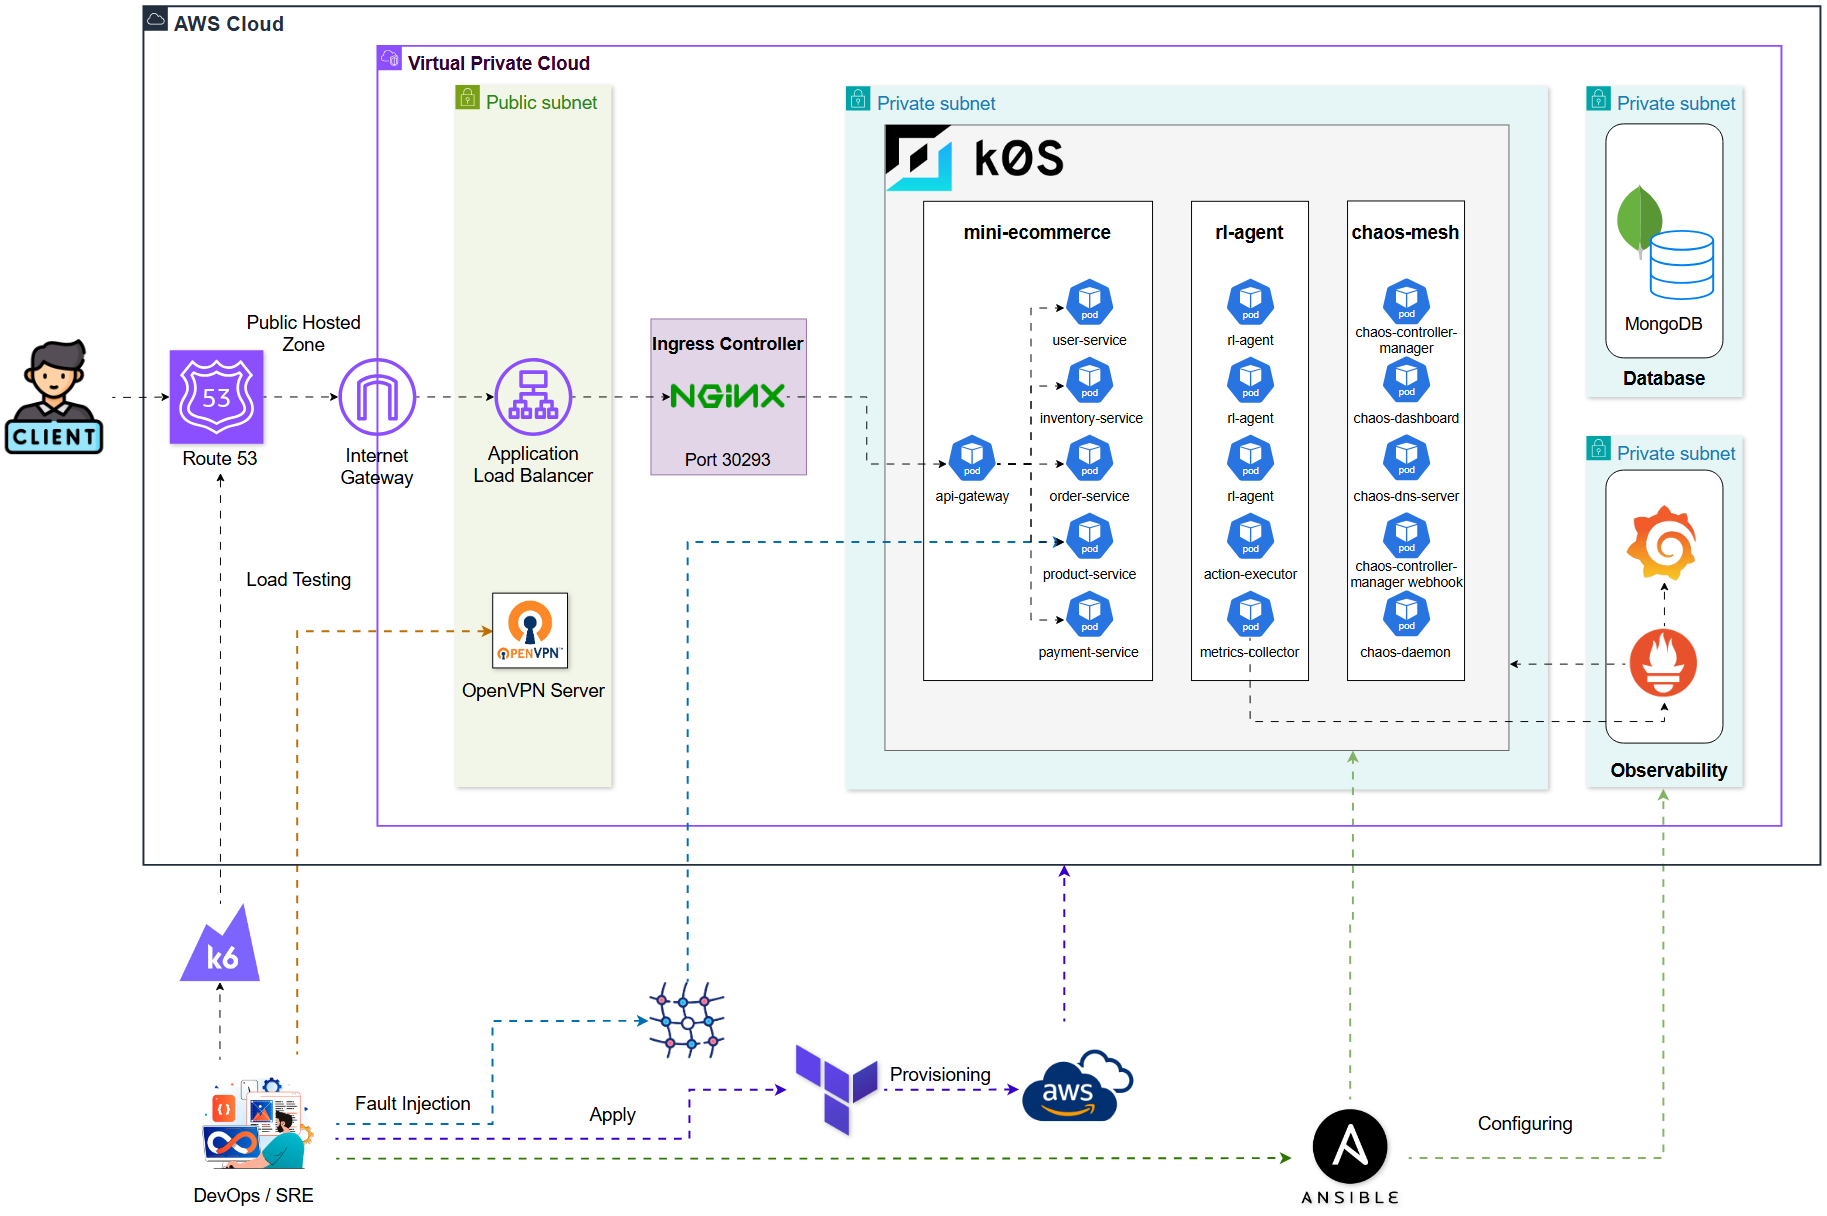
\includegraphics[width=1.0\textwidth]{graphics/chapter-5/5_0_architecture/architecture_diagram.png}
    \caption{Kiến trúc tổng thể môi trường triển khai và thực nghiệm của hệ thống}
    \label{fig:overall-system-architecture}
\end{figure}

\noindent Từ góc nhìn vận hành, người dùng và tải kiểm 
thử được định tuyến qua Route 53, Internet Gateway, 
Application Load Balancer và NGINX Ingress trước khi 
đi vào cụm \texttt{k0s}. Bên trong cụm, ứng dụng 
\textit{mini-ecommerce} đóng vai trò workload chính 
để sinh lưu lượng và sự cố phục vụ đánh giá khả năng 
tự phục hồi. Song song đó, namespace \texttt{rl-agent} 
đảm nhiệm việc thu thập trạng thái, suy luận hành động và 
thực thi can thiệp phục hồi, trong khi Chaos Mesh chịu 
trách nhiệm kích hoạt các kịch bản lỗi có kiểm soát.

\noindent Sơ đồ cũng cho thấy rõ mối liên hệ giữa các 
công cụ tự động hóa và giám sát trong toàn bộ pipeline 
triển khai. Terraform được sử dụng để khởi tạo tài nguyên 
trên AWS, Ansible tiếp tục cấu hình các máy chủ và dịch vụ 
nền, Prometheus/Grafana đảm nhiệm lớp observability, còn 
K6 cung cấp tải kiểm thử để tạo dữ liệu đánh giá. Nhờ đó, 
môi trường thực nghiệm không chỉ phản ánh cấu trúc triển 
khai thực tế mà còn hỗ trợ đầy đủ cho các pha benchmark, 
fault injection, thu thập metrics và đánh giá cơ chế 
self-healing dựa trên học tăng cường.

\section{Thiết kế cơ sở hạ tầng trên nền tảng AWS}

Môi trường thực nghiệm được thiết kế và triển khai trên 
nền tảng Amazon Web Services (AWS) nhằm đảm bảo tính linh 
hoạt, khả năng mở rộng tự động và mức độ sẵn sàng cao 
(High Availability). Kiến trúc hệ thống phân bổ dịch vụ 
trên nhiều Vùng khả dụng (Availability Zones - AZs) trong 
cùng một VPC (Virtual Private Cloud) để triệt tiêu các 
điểm lỗi đơn lẻ (SPoF) và tối ưu hóa khả năng chịu lỗi 
vật lý.

Chi tiết mô hình kiến trúc hạ tầng AWS được minh họa cụ thể trong Hình \ref{fig:aws-infra-architecture}.

\begin{figure}[htbp]
    \centering
    \includegraphics[width=1.0\textwidth]{graphics/chapter-5/cloud.png}
    \caption{Kiến trúc triển khai cơ sở hạ tầng trên nền tảng AWS}
    \label{fig:aws-infra-architecture}
\end{figure}

Kiến trúc hạ tầng bao gồm ba lớp chức năng chính:
\begin{itemize}
    \item \textbf{Lớp mạng (Networking Layer):} VPC dải 
    mạng \texttt{10.0.0.0/16} được chia làm các Public/Private 
    Subnet trên 03 AZs (us-east-1a, us-east-1b, us-east-1c). 
    Lớp này sử dụng Internet Gateway (IGW) cho kết nối ngoài, 
    NAT Gateway bảo mật cho phân vùng nội bộ, và Application 
    Load Balancer (ALB) điều phối lưu lượng từ phía người dùng 
    vào các dịch vụ bên trong hệ thống.
    \item \textbf{Lớp tính toán (Compute Layer):} Cụm Kubernetes được phân bổ trên cả 03 AZs để vận hành workloads. Trong đó, Master node đặt tại Private Subnet của AZ 1, các Worker node được phân tán ở các AZs khác nhau. Ngoài ra, hệ thống được bổ sung thêm Auto Scaling Group giúp hỗ trợ tăng giảm số máy Worker phục vụ lượng tải linh hoạt từ người dùng.
    \item \textbf{Lớp giám sát và quản trị (Management Layer):} Tích hợp Prometheus để thu thập dữ liệu huấn luyện (metrics) thời gian thực và Grafana để trực quan hóa phục vụ phân tích. Hệ thống quản trị được bảo mật thông qua OpenVPN Server đặt tại Public Subnet của AZ 3.
\end{itemize}

Để tối ưu hóa luồng lưu lượng và đảm bảo tính cô lập an toàn, 
địa chỉ IP được phân hoạch chi tiết cho toàn bộ các phân vùng 
mạng (Subnets) trong hệ thống như. Chi tiết được trình bày trong 
Bảng \ref{tab:subnet-ip-allocation}.

\begin{center}
\captionof{table}{Phân hoạch địa chỉ IP cho các Subnets trong hệ thống thực nghiệm}
\label{tab:subnet-ip-allocation}
\footnotesize
\renewcommand{\arraystretch}{1.0}
\begin{tabular}{|C{3.2cm}|C{2.8cm}|C{3.0cm}|L{6.0cm}|}
\hline
\textbf{Vùng khả dụng (AZ)} & \textbf{Loại Subnet} & \textbf{Dải địa chỉ (CIDR)} & \textbf{Thành phần được triển khai} \\ \hline
\multirow{3}{*}{us-east-1a (AZ 1)} & Public & 10.0.1.0/24 & ALB ENI, NAT Gateway \\ \cline{2-4} 
 & Private (k0s) & 10.0.11.0/24 & k0s Master, k0s Worker Node \\ \cline{2-4} 
 & Private (Data) & 10.0.21.0/24 & Prometheus, Grafana \\ \hline
\multirow{3}{*}{us-east-1b (AZ 2)} & Public & 10.0.2.0/24 & ALB ENI \\ \cline{2-4} 
 & Private (k0s) & 10.0.12.0/24 & k0s Worker Node (Auto Scaling) \\ \cline{2-4} 
 & Private (Data) & 10.0.22.0/24 & Phân vùng dự phòng (Unused) \\ \hline
\multirow{3}{*}{us-east-1c (AZ 3)} & Public & 10.0.3.0/24 & OpenVPN Access Server \\ \cline{2-4} 
 & Private (k0s) & 10.0.13.0/24 & k0s Worker Node \\ \cline{2-4} 
 & Private (Data) & 10.0.23.0/24 & Phân vùng dự phòng (Unused) \\ \hline
\end{tabular}
\end{center}

Cơ sở hạ tầng mạng và tính toán này thiết lập một môi 
trường thực nghiệm có tính chân thực cao, tương đương 
với các hệ thống Cloud Production. Đây là nền tảng cốt 
lõi để thực hiện các kịch bản kích hoạt sự cố nhân tạo 
(Chaos Injection) liên quan đến \textit{Pod failure}, 
từ đó đo lường chính xác thời gian phục hồi và độ ổn định 
của giải pháp đề xuất so với cơ chế mặc định của Kubernetes.

\section{Triển khai cơ sở hạ tầng sử dụng Terraform}

Để đảm bảo tính tự động hóa, tính nhất quán và khả năng tái lập nhanh chóng cho môi trường thực nghiệm, toàn bộ tài nguyên hạ tầng trên AWS được định nghĩa và khởi tạo dưới dạng mã nguồn (Infrastructure as Code - IaC) thông qua công cụ Terraform. Việc này giúp triệt tiêu các sai sót cấu hình thủ công và kiểm soát chặt chẽ trạng thái tài nguyên thông qua tệp tin \texttt{terraform.tfstate}.


Quy trình áp dụng hạ tầng được thực hiện qua các lệnh tiêu chuẩn của Terraform bao gồm: \texttt{terraform init} (khởi tạo môi trường), \texttt{terraform plan} (kiểm tra dự báo thay đổi) và \texttt{terraform apply} (thực thi khởi tạo thực tế trên AWS). 



\noindent Sau bước khởi tạo mã nguồn hạ tầng, tác giả tiến hành kiểm tra lại đầu ra của lệnh apply, trạng thái các máy ảo đang hoạt động và cuối cùng là cấu trúc mạng đã được dựng lên trên AWS để bảo đảm trạng thái triển khai khớp với thiết kế mong muốn.

\begin{center}
    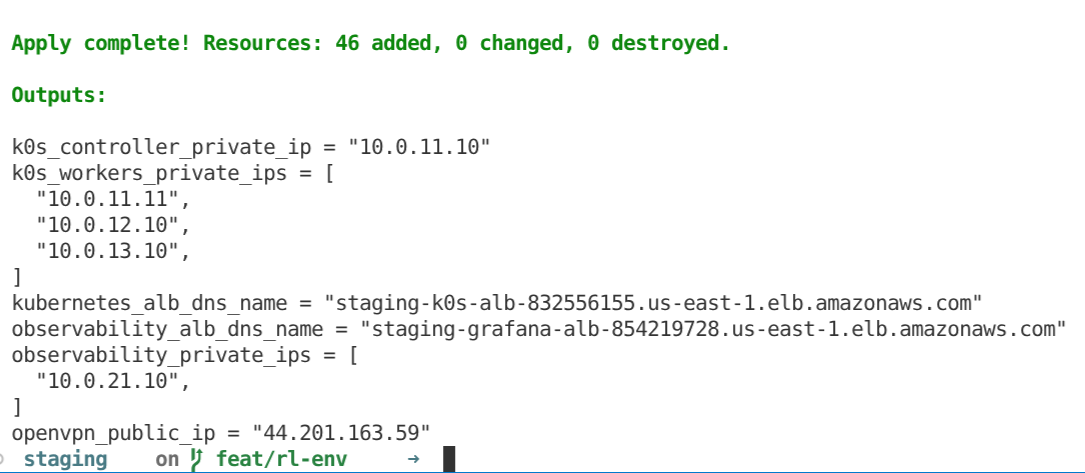
\includegraphics[width=0.92\textwidth]{graphics/chapter-5/5_1_infra/terraform_apply.png}
    \captionof{figure}{Đầu ra sau khi thực thi \texttt{terraform apply}}
    \label{fig:terraform-apply-output}
\end{center}

\noindent Hình \ref{fig:terraform-apply-output} ghi nhận kết quả \texttt{46 added, 0 changed, 0 destroyed}, cho thấy toàn bộ tài nguyên hạ tầng đã được tạo mới thành công và không phát sinh sai lệch trạng thái trong lần apply này. Các output quan trọng như địa chỉ IP private của controller, danh sách IP của các worker, DNS của Application Load Balancer và địa chỉ public của máy chủ OpenVPN đều được Terraform xuất ra ngay sau khi hoàn tất. Đây là tập thông tin đầu vào quan trọng để chuyển sang bước cấu hình tiếp theo bằng Ansible.

\begin{center}
    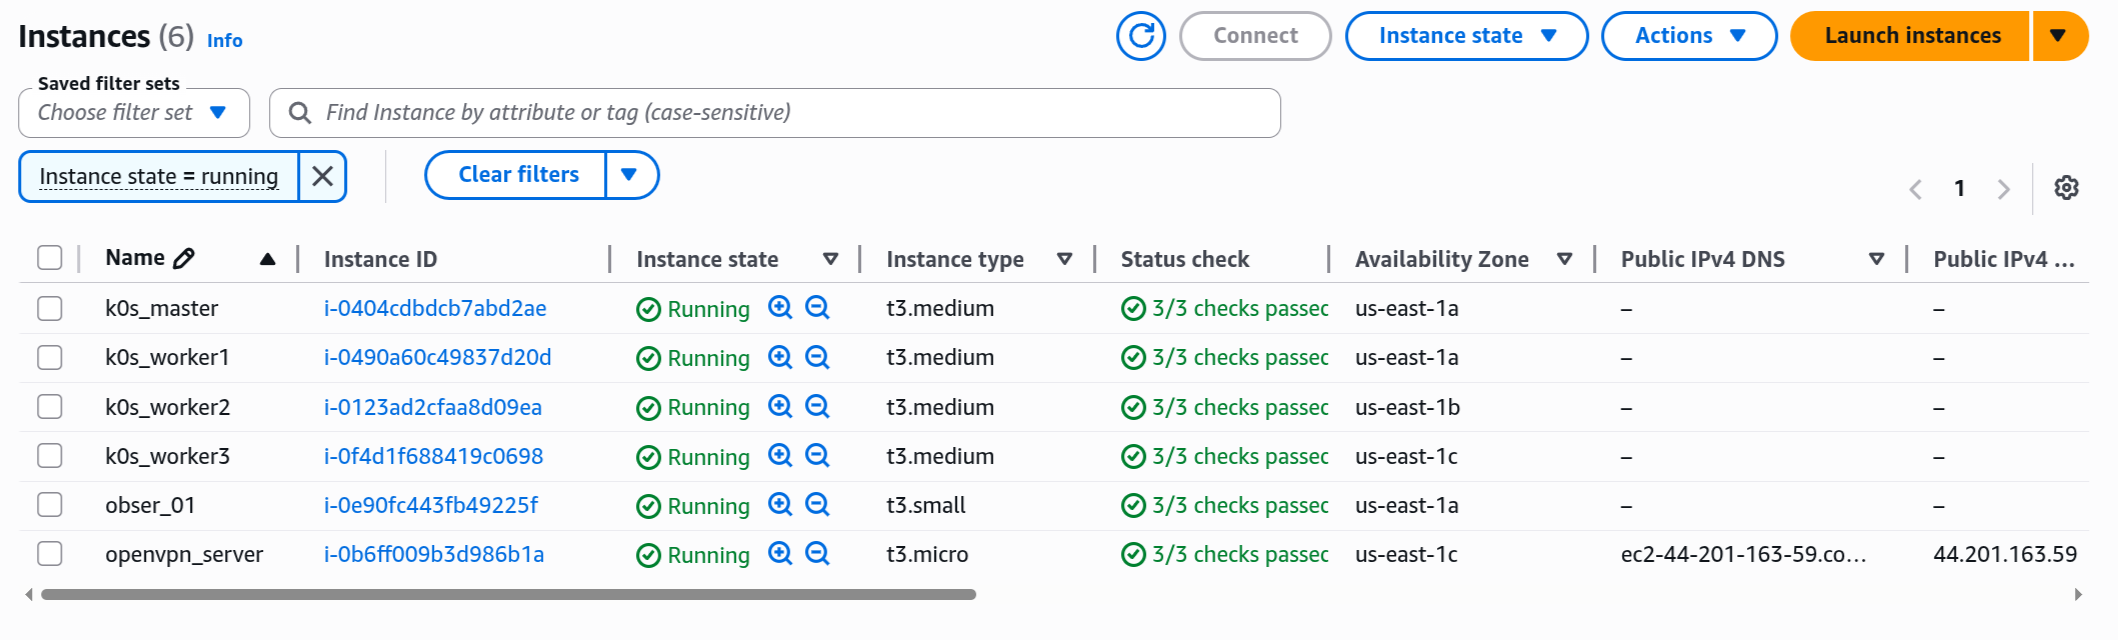
\includegraphics[width=1.0\textwidth]{graphics/chapter-5/5_1_infra/ec2.png}
    \captionof{figure}{Các máy ảo EC2 được Terraform khởi tạo và đưa về trạng thái hoạt động}
    \label{fig:terraform-ec2-running}
\end{center}

\noindent Hình \ref{fig:terraform-ec2-running} xác nhận các máy ảo chính của môi trường thực nghiệm đã được tạo và đi vào trạng thái \textit{Running}, bao gồm một node \texttt{k0s\_master}, ba worker \texttt{k0s\_worker1}, \texttt{k0s\_worker2}, \texttt{k0s\_worker3}, một máy chủ giám sát \texttt{observ\_01} và một máy \texttt{openvpn\_server}. Toàn bộ instance đều vượt qua \textit{status check}, đồng thời được phân bố trên các Availability Zone đúng theo thiết kế hạ tầng đã mô tả ở phần trước. Kết quả này cho thấy lớp cơ sở hạ tầng đã sẵn sàng để tiếp tục cấu hình cụm Kubernetes, công cụ giám sát và môi trường thí nghiệm cho bài toán self-healing.

\begin{center}
    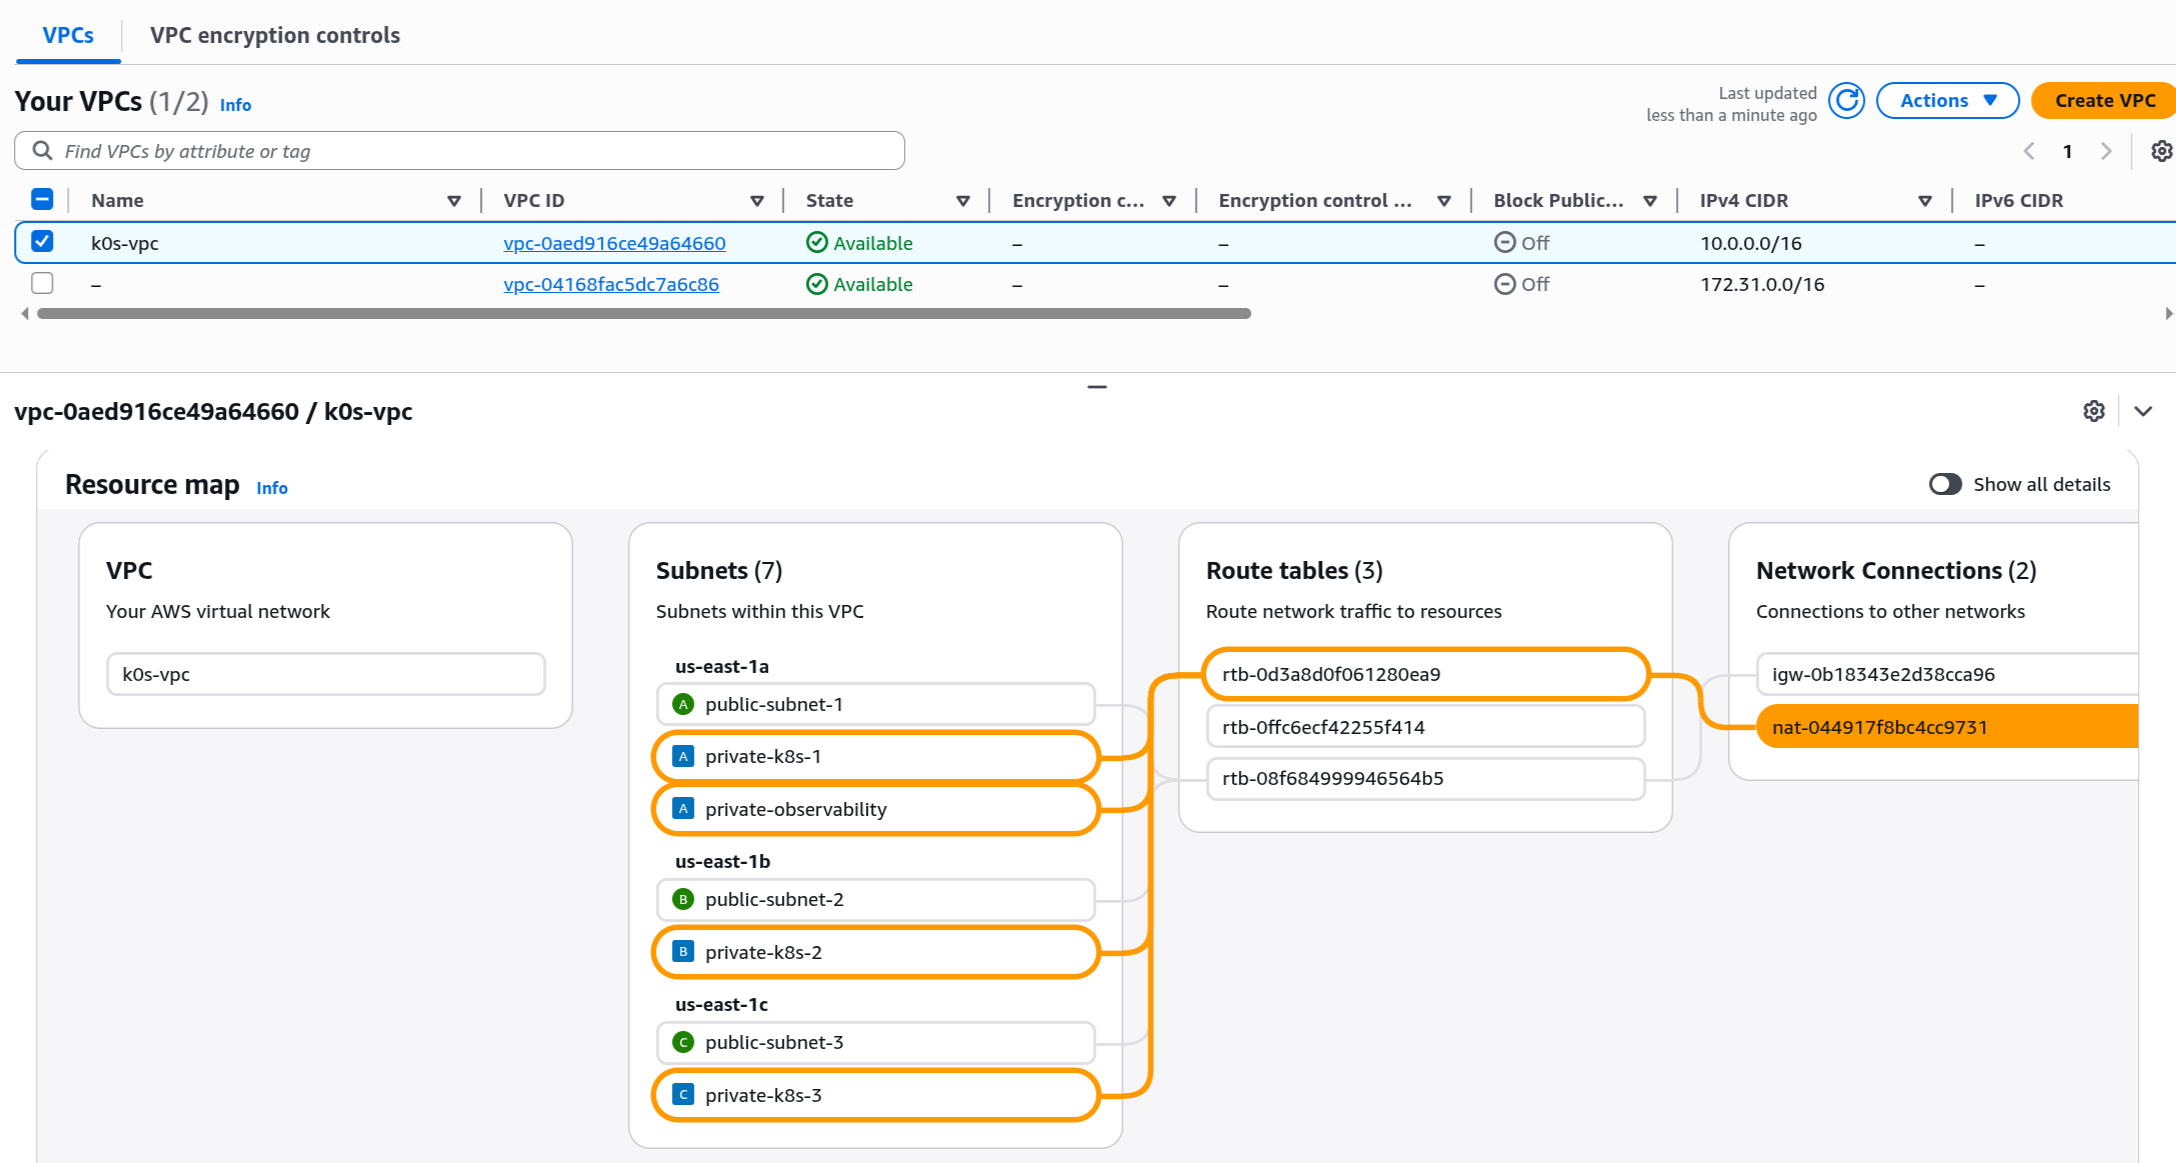
\includegraphics[width=1.0\textwidth]{graphics/chapter-5/5_1_infra/vpc.png}
    \captionof{figure}{Cấu trúc VPC và các subnet được Terraform khởi tạo trên AWS}
    \label{fig:terraform-vpc-topology}
\end{center}

\noindent Hình \ref{fig:terraform-vpc-topology} cho thấy Terraform đã khởi tạo thành công VPC với dải mạng 10.0.0.0/16, đồng thời phân tách rõ public subnet và private subnet trên ba Availability Zone.

\noindent Các subnet dành cho cụm Kubernetes gồm:
\begin{itemize}
    \item \texttt{private-k8s-1}
    \item \texttt{private-k8s-2}
    \item \texttt{private-k8s-3}
\end{itemize}
\noindent Trong khi đó, subnet \texttt{private-observability} 
được sử dụng cho Prometheus và Grafana. Việc định tuyến private subnet 
thông qua NAT Gateway giúp các máy nội bộ có thể truy cập ra ngoài khi 
cần cài đặt và cập nhật gói, nhưng vẫn giữ được nguyên tắc không phơi lộ 
trực tiếp ra Internet.

\section{Cấu hình các công cụ sử dụng Ansible}

Để tự động hóa cấu hình hệ điều hành và thiết lập phần mềm trên các máy chủ EC2 
đã được khởi tạo bởi Terraform, công cụ Ansible được sử dụng. Với kiến trúc 
không tác nhân (\textit{agentless}), Ansible thực hiện truyền tải các cấu hình 
thông qua kết nối SSH bảo mật, giúp thiết lập môi trường đồng bộ, nhất quán và giảm thiểu tối đa các thao tác quản trị thủ công. Các chỉ thị cấu hình được khai báo dưới dạng tệp tin YAML (\textit{Ansible Playbooks}).

\subsection{Cấu hình dịch vụ mạng riêng ảo sử dụng OpenVPN}

Dịch vụ OpenVPN Server được cấu hình và thiết lập tự động thông qua Ansible trên máy chủ đặt tại Public Subnet của AZ 3. Vai trò của thành phần này là thiết lập một đường truyền mã hóa bảo mật từ xa (VPN Tunnel) cho phép quản trị viên truy cập an toàn vào dải mạng nội bộ (Private Subnet) của VPC để thực hiện các thao tác quản trị cụm Kubernetes và hệ thống giám sát mà không cần công khai các cổng dịch vụ ra Internet.

Một phần cấu hình chính của OpenVPN được khai báo như sau:

\begin{lstlisting}
# OpenVPN basic
openvpn_port: 1194
openvpn_proto: udp

# VPN network
openvpn_network: 10.8.0.0
openvpn_netmask: 255.255.255.0
openvpn_tunnel_iface: tun0

# Directories
openvpn_server_dir: /etc/openvpn/server
easy_rsa_dir: /etc/openvpn/easy-rsa

# Client
openvpn_client_name: devops
openvpn_public_ip: "{{ ansible_host }}"

# EC2 private interface (AWS Ubuntu)
openvpn_private_iface: ens5

# ===== VPC ROUTE =====
# CIDR cua VPC PROD
vpc_network: 10.0.0.0
vpc_netmask: 255.255.0.0

# DNS for client
openvpn_dns:
  - 8.8.8.8
  - 1.1.1.1
\end{lstlisting}

\noindent Về mặt định tuyến, OpenVPN tạo một mạng tunnel riêng với dải \texttt{10.8.0.0/24} trên interface \texttt{tun0}. Khi máy khách kết nối vào VPN, lưu lượng quản trị sẽ đi trước hết vào tunnel này, sau đó được máy chủ OpenVPN chuyển tiếp sang card mạng private \texttt{ens5} để truy cập các tài nguyên nằm trong VPC nội bộ.

\noindent Cặp tham số \texttt{vpc\_network=10.0.0.0} và \texttt{vpc\_netmask=255.255.0.0} là phần quan trọng nhất của cấu hình routing, vì nó xác định đích đến cuối cùng của các gói tin từ phía client. Nói cách khác, OpenVPN phải biết rằng mọi lưu lượng hướng tới dải \texttt{10.0.0.0/16} cần được đẩy vào mạng VPC thay vì đi ra Internet công cộng. Nhờ đó, sau khi kết nối VPN, quản trị viên có thể truy cập các máy \texttt{k0s\_master}, \texttt{k0s\_worker*} và máy giám sát bằng địa chỉ private mà không cần mở cổng SSH trực tiếp ra ngoài.

\noindent Cách cấu hình này mang lại hai lợi ích chính. Thứ nhất, lớp quản trị được tách biệt khỏi luồng truy cập của người dùng cuối, giúp giảm bề mặt tấn công lên cụm thực nghiệm. Thứ hai, toàn bộ thao tác Ansible, SSH và kiểm tra dịch vụ nội bộ đều có thể thực hiện thông qua VPN, bảo đảm đúng nguyên tắc chỉ cho phép truy cập riêng tư vào các subnet vận hành Kubernetes và observability.

\subsection{Cấu hình cụm Kubernetes}

Quy trình thiết lập cụm Kubernetes được tự động hóa hoàn toàn bằng Ansible Playbook bao gồm các công đoạn chính:
\begin{itemize}
    \item \textbf{Chuẩn bị môi trường:} Tắt phân vùng swap, cấu hình các tham số nhân hệ điều hành (\textit{sysctl}) cho mạng container và cài đặt container runtime (như \texttt{containerd}).
    \item \textbf{Cấu hình Master Node:} Khởi tạo nút điều khiển (Control Plane), thiết lập tệp cấu hình \texttt{kubeconfig} và cài đặt Container Network Interface (CNI) để thiết lập mạng nội bộ cho các Pods.
    \item \textbf{Gia nhập các Worker Nodes:} Ansible tự động trích xuất mã thông báo gia nhập (\textit{join token}) từ Master Node và thực thi lệnh kết nối các Worker Nodes phân tán trên các AZs vào cụm.
\end{itemize}

\begin{center}
    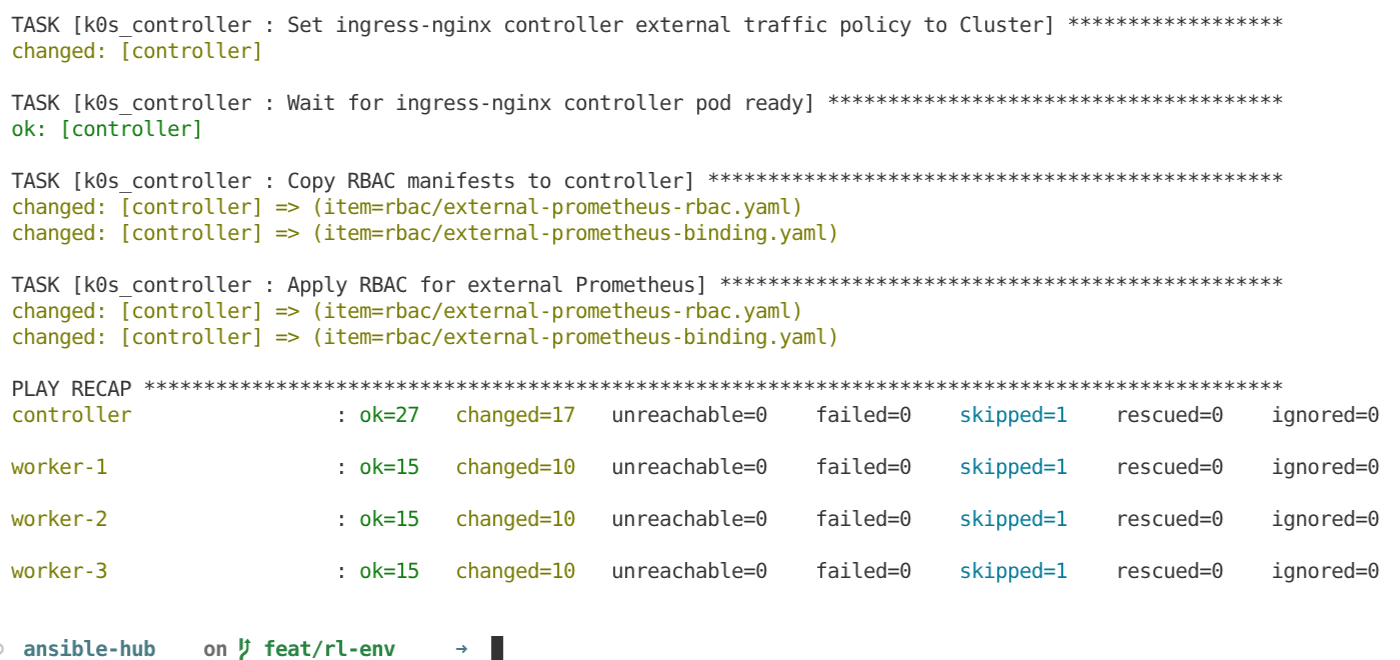
\includegraphics[width=1.0\textwidth]{graphics/chapter-5/5_2_kubernetes/config_k0s.png}
    \captionof{figure}{Kết quả chạy Ansible Playbook để cấu hình cụm k0s và RBAC cho Prometheus}
    \label{fig:k0s-ansible-config}
\end{center}

\noindent Hình \ref{fig:k0s-ansible-config} cho thấy quá trình Ansible thực thi các tác vụ cấu hình trên nút controller, bao gồm thiết lập ingress-nginx, chờ Pod sẵn sàng và áp dụng RBAC cho external Prometheus. Phần \texttt{PLAY RECAP} xác nhận toàn bộ các máy \texttt{controller}, \texttt{worker-1}, \texttt{worker-2} và \texttt{worker-3} đều hoàn tất không có lỗi, thể hiện việc triển khai cụm Kubernetes đã được tự động hóa ổn định và lặp lại được.

\begin{center}
    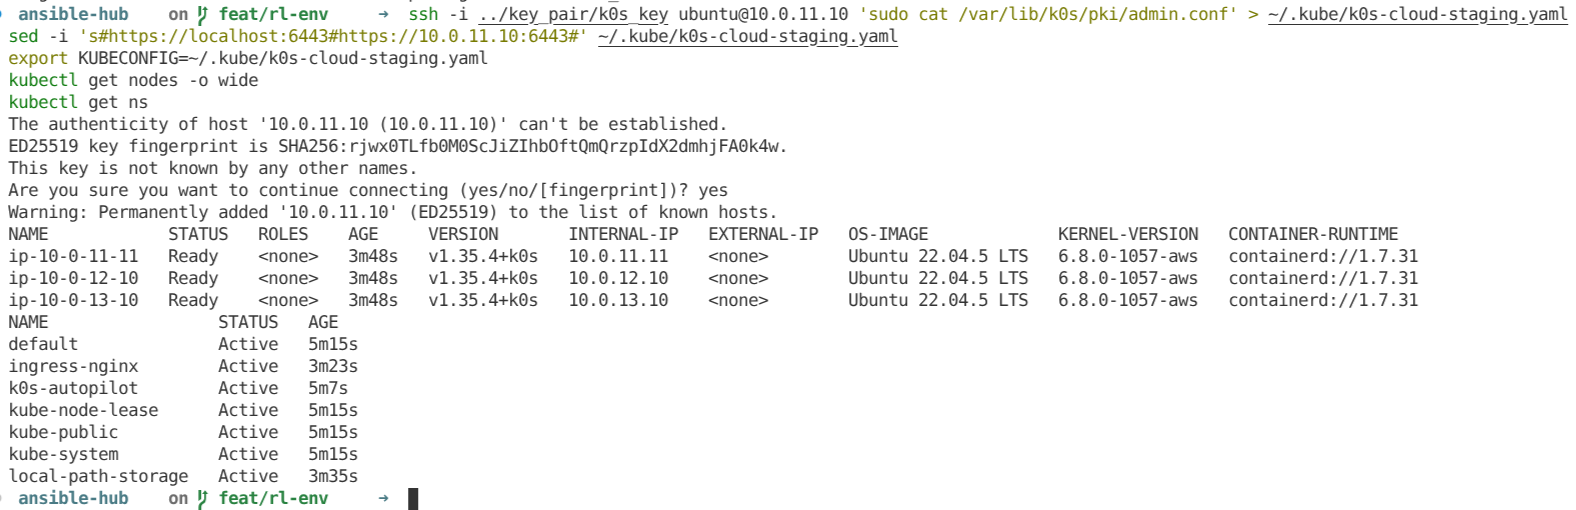
\includegraphics[width=1.0\textwidth]{graphics/chapter-5/5_2_kubernetes/connect_cluster.png}
    \captionof{figure}{Kết nối vào cụm k0s và kiểm tra trạng thái node, namespace sau triển khai}
    \label{fig:k0s-cluster-connect}
\end{center}

\noindent Từ Hình \ref{fig:k0s-cluster-connect}, có thể thấy tệp \texttt{kubeconfig} được trích xuất từ controller và hiệu chỉnh để truy cập qua địa chỉ private \texttt{10.0.11.10:6443}. Kết quả \texttt{kubectl get nodes -o wide} xác nhận ba worker node đã ở trạng thái \texttt{Ready}, đồng thời các namespace hệ thống như \texttt{default}, \texttt{kube-system}, \texttt{ingress-nginx} và \texttt{local-path-storage} đều ở trạng thái \texttt{Active}. Điều này cho thấy cụm Kubernetes đã sẵn sàng làm nền tảng triển khai microservices, giám sát và tác nhân RL ở các bước tiếp theo.

\subsection{Cấu hình hệ thống giám sát sử dụng Prometheus và Grafana}

Hệ thống giám sát được cấu hình tập trung trên máy chủ chuyên dụng đặt tại Private Subnet của AZ 1 nhằm đảm bảo tính toàn vẹn dữ liệu:
\begin{itemize}
    \item \textbf{Prometheus:} Được cấu hình thông qua Ansible để tự động phát hiện dịch vụ (\textit{service discovery}) trong cụm Kubernetes, thu thập dữ liệu metrics từ \texttt{node-exporter} (được Ansible cài đặt trên từng node) và \texttt{kube-state-metrics} theo chu kỳ 5 giây.
    \item \textbf{Grafana:} Được cấu hình sẵn các nguồn dữ liệu (\textit{Data Sources}) kết nối trực tiếp tới Prometheus và tự động nạp các bảng giao diện trực quan hóa (\textit{Dashboards}) để theo dõi hiệu năng tài nguyên hệ thống (CPU, RAM, Network) theo thời gian thực.
\end{itemize}

\begin{center}
    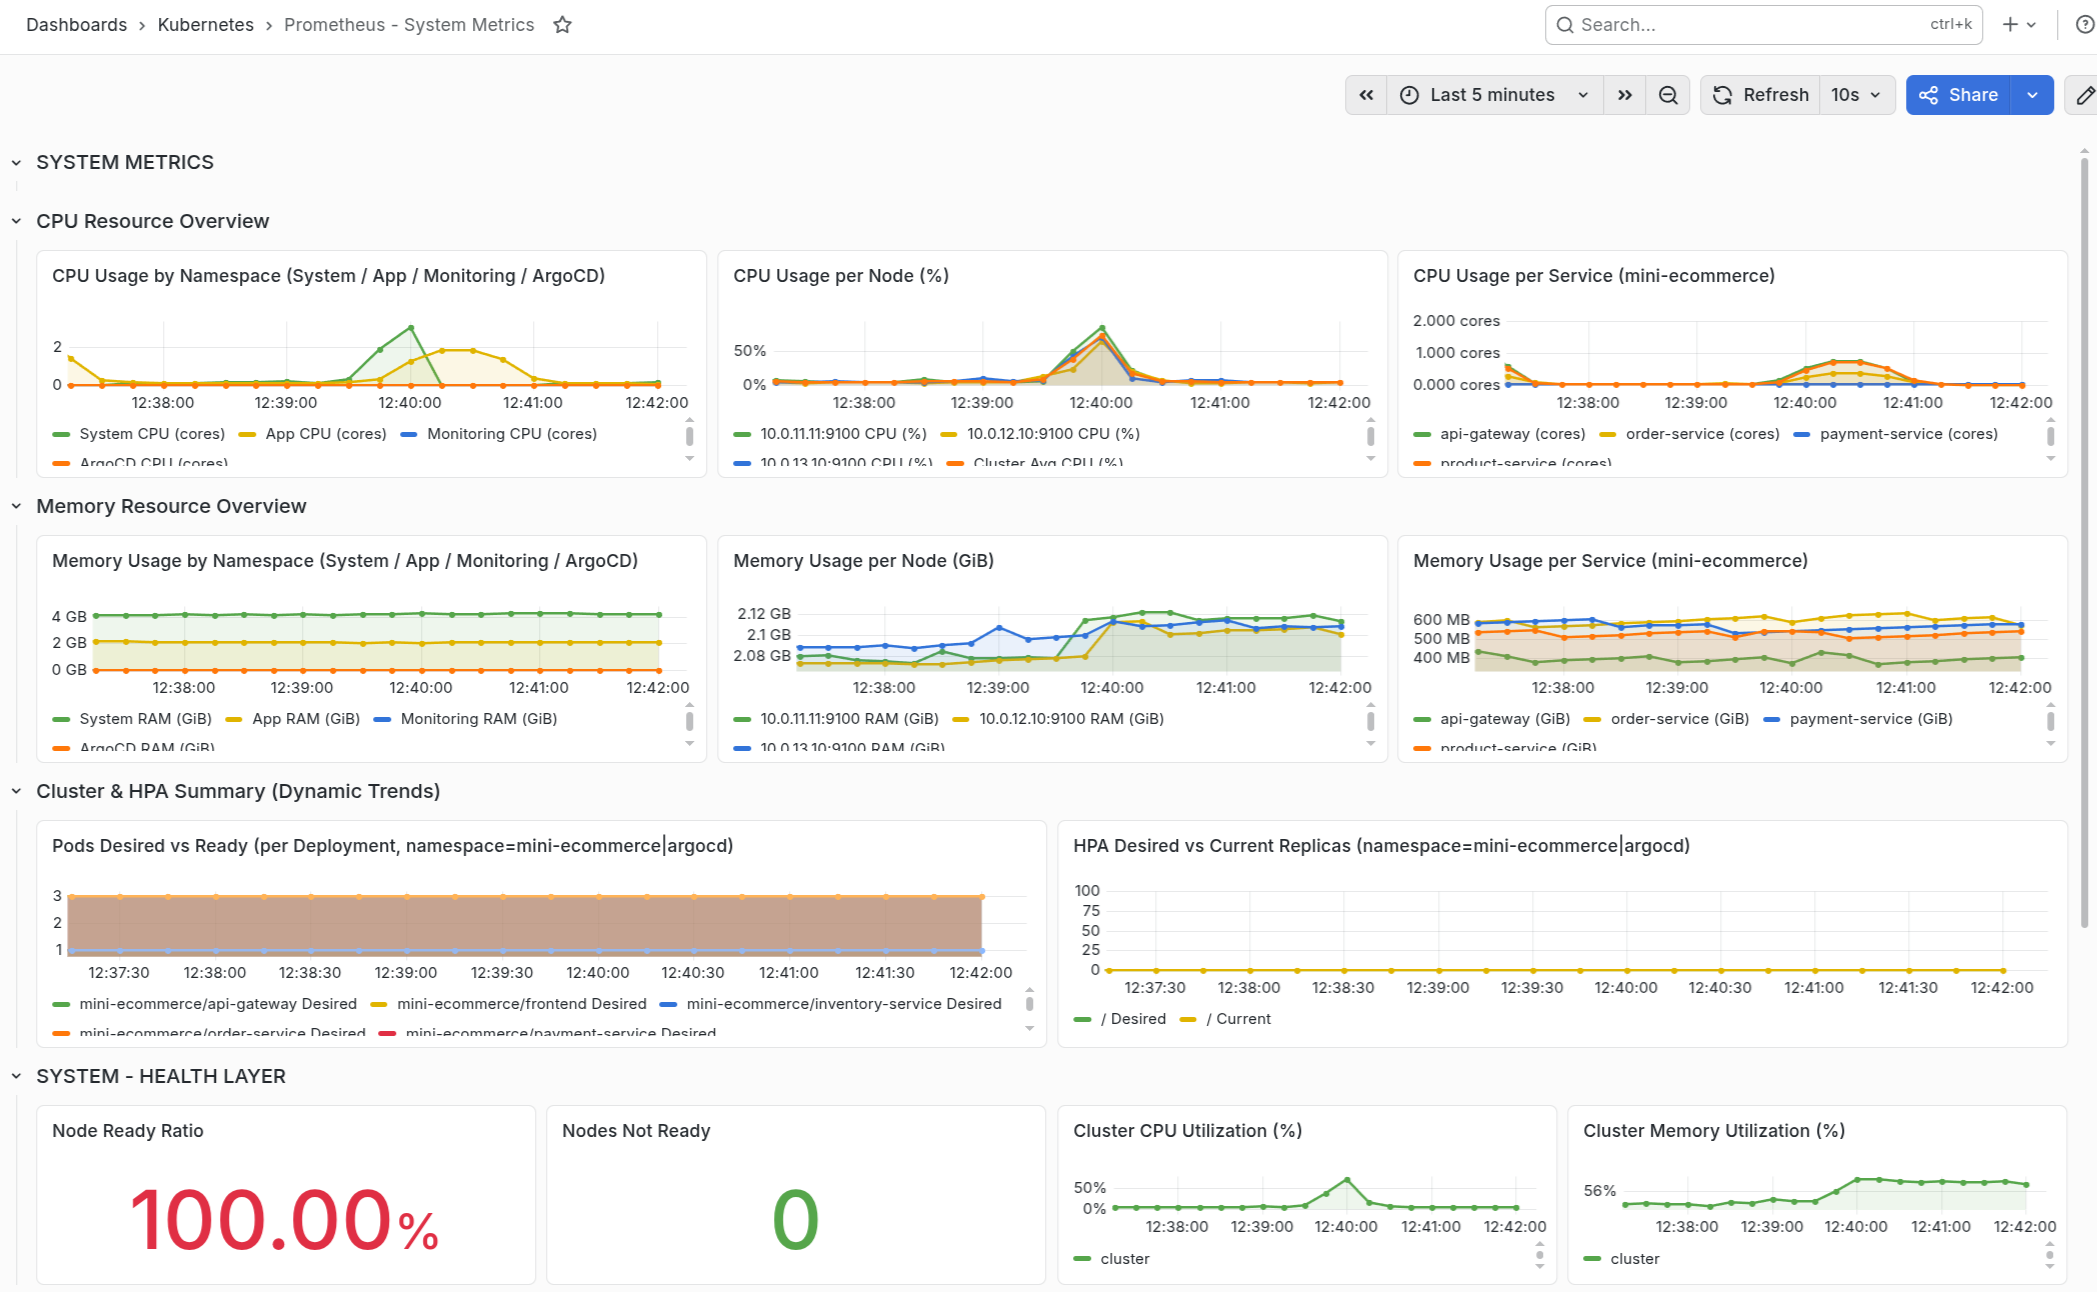
\includegraphics[width=1.0\textwidth]{graphics/chapter-5/5_3_monitoring/grafama_dashboard.png}
    \captionof{figure}{Dashboard Grafana theo dõi tài nguyên hệ thống và trạng thái dịch vụ}
    \label{fig:grafana-monitoring-dashboard}
\end{center}

\noindent Hình \ref{fig:grafana-monitoring-dashboard} cho thấy giao diện dashboard Grafana sau khi kết nối trực tiếp tới Prometheus. Các biểu đồ được tổ chức để theo dõi đồng thời tài nguyên hạ tầng, trạng thái Pod, độ trễ và các chỉ số phục vụ phân tích self-healing. Đây cũng là lớp quan sát trực quan giúp đối chiếu nhanh giữa thời điểm xảy ra sự cố, phản ứng của hệ thống và dữ liệu được xuất ra cho bước huấn luyện RL.

\section{Triển khai ứng dụng Microservices}

\subsection{Tổng quan ứng dụng}

Ứng dụng được sử dụng trong đồ án là hệ thống \textit{Mini Ecommerce Microservices} do tác giả tự phát triển, được xây dựng theo kiến trúc microservices đa ngôn ngữ nhằm phục vụ đồng thời cho thực nghiệm DevOps, observability và học tăng cường. Hệ thống mô phỏng một quy trình thương mại điện tử thu gọn, trong đó người dùng có thể đăng nhập, xem sản phẩm, kiểm tra tồn kho và tạo đơn hàng thông qua một điểm vào duy nhất là \texttt{api-gateway}.

\begin{center}
    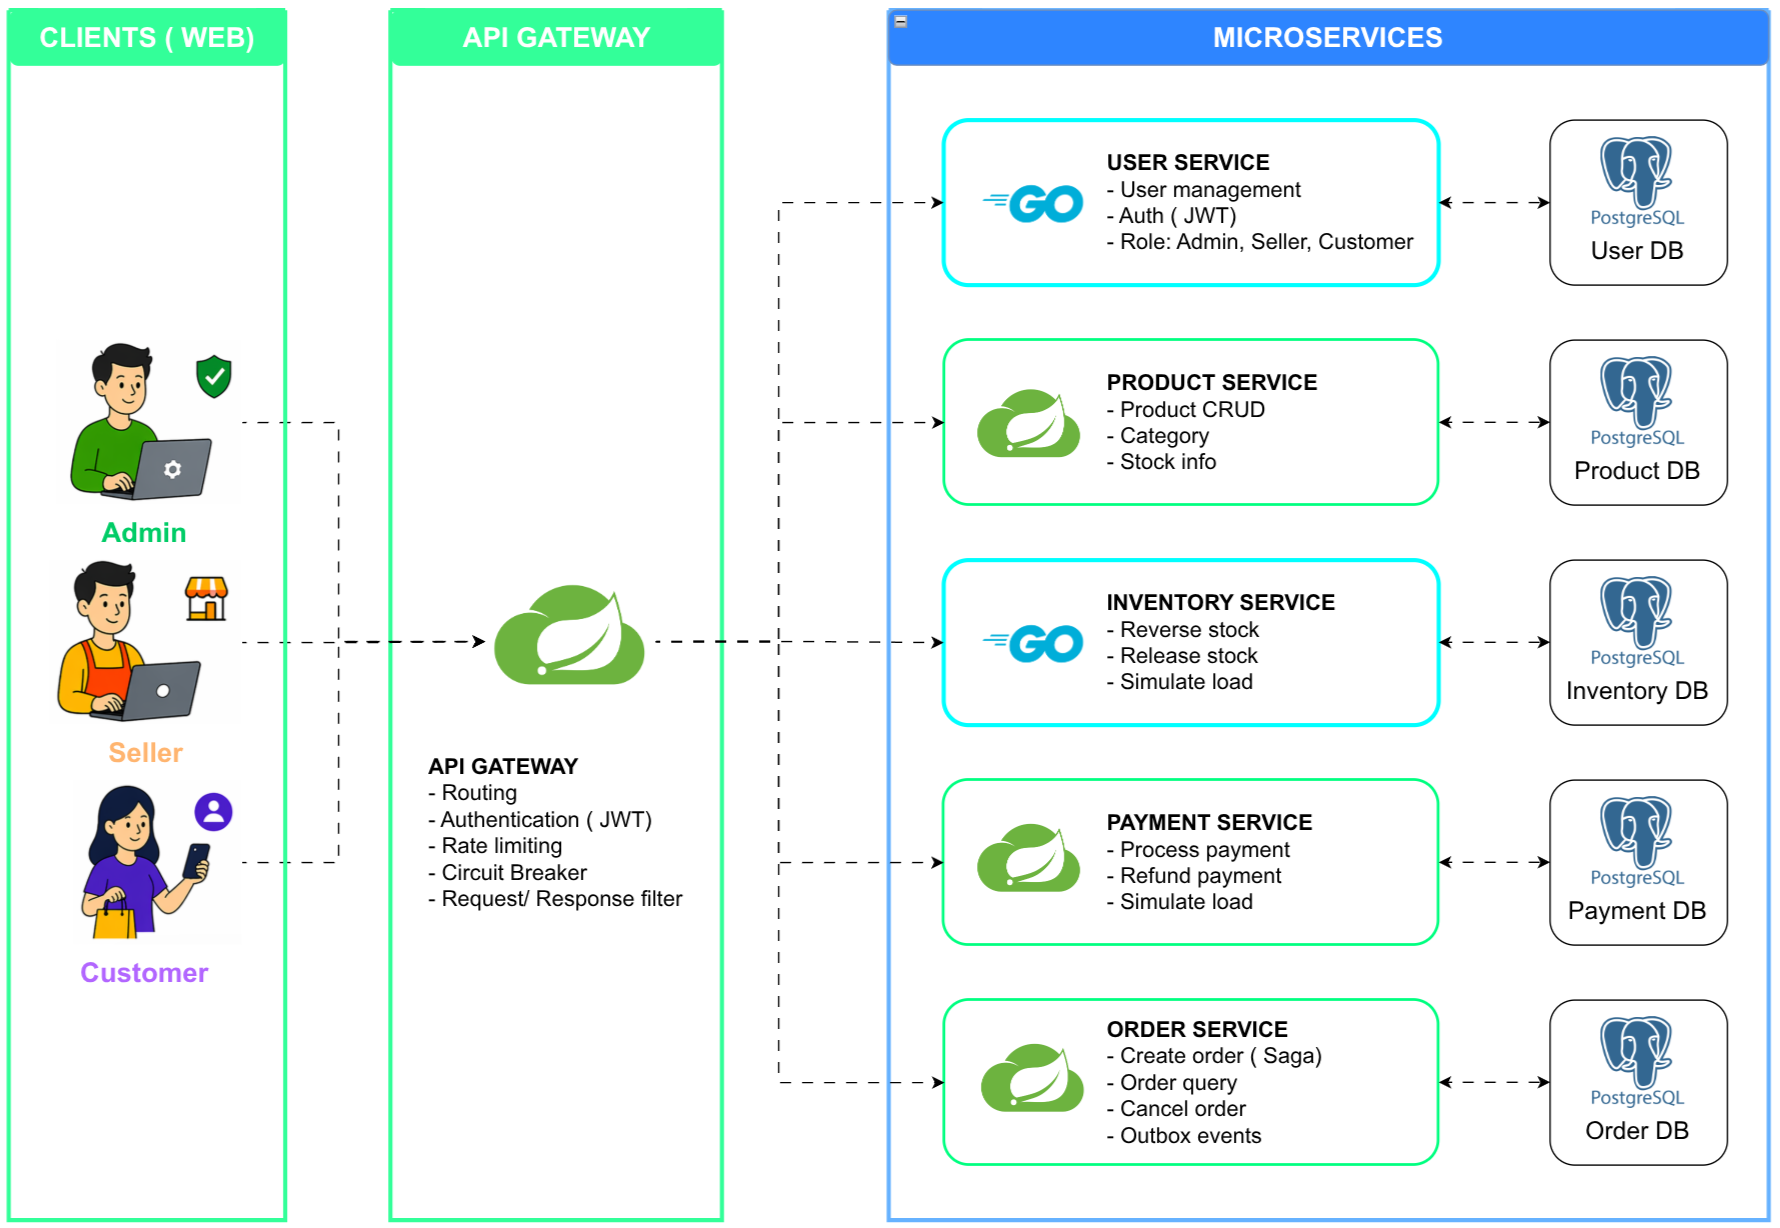
\includegraphics[width=0.97\textwidth]{graphics/chapter-5/5_4_application/architecture.png}
    \captionof{figure}{Kiến trúc tổng quan của ứng dụng Mini Ecommerce Microservices}
    \label{fig:mini-ecommerce-architecture}
\end{center}

\noindent Hình \ref{fig:mini-ecommerce-architecture} minh họa luồng truy cập từ phía người dùng qua \texttt{api-gateway} tới các microservice nghiệp vụ và cơ sở dữ liệu tương ứng. Kiến trúc này thể hiện rõ vai trò của gateway như lớp định tuyến và kiểm soát truy cập tập trung, trong khi các service phía sau được tách biệt theo miền chức năng để bảo đảm tính độc lập khi triển khai, giám sát và phục hồi.

\begin{center}
    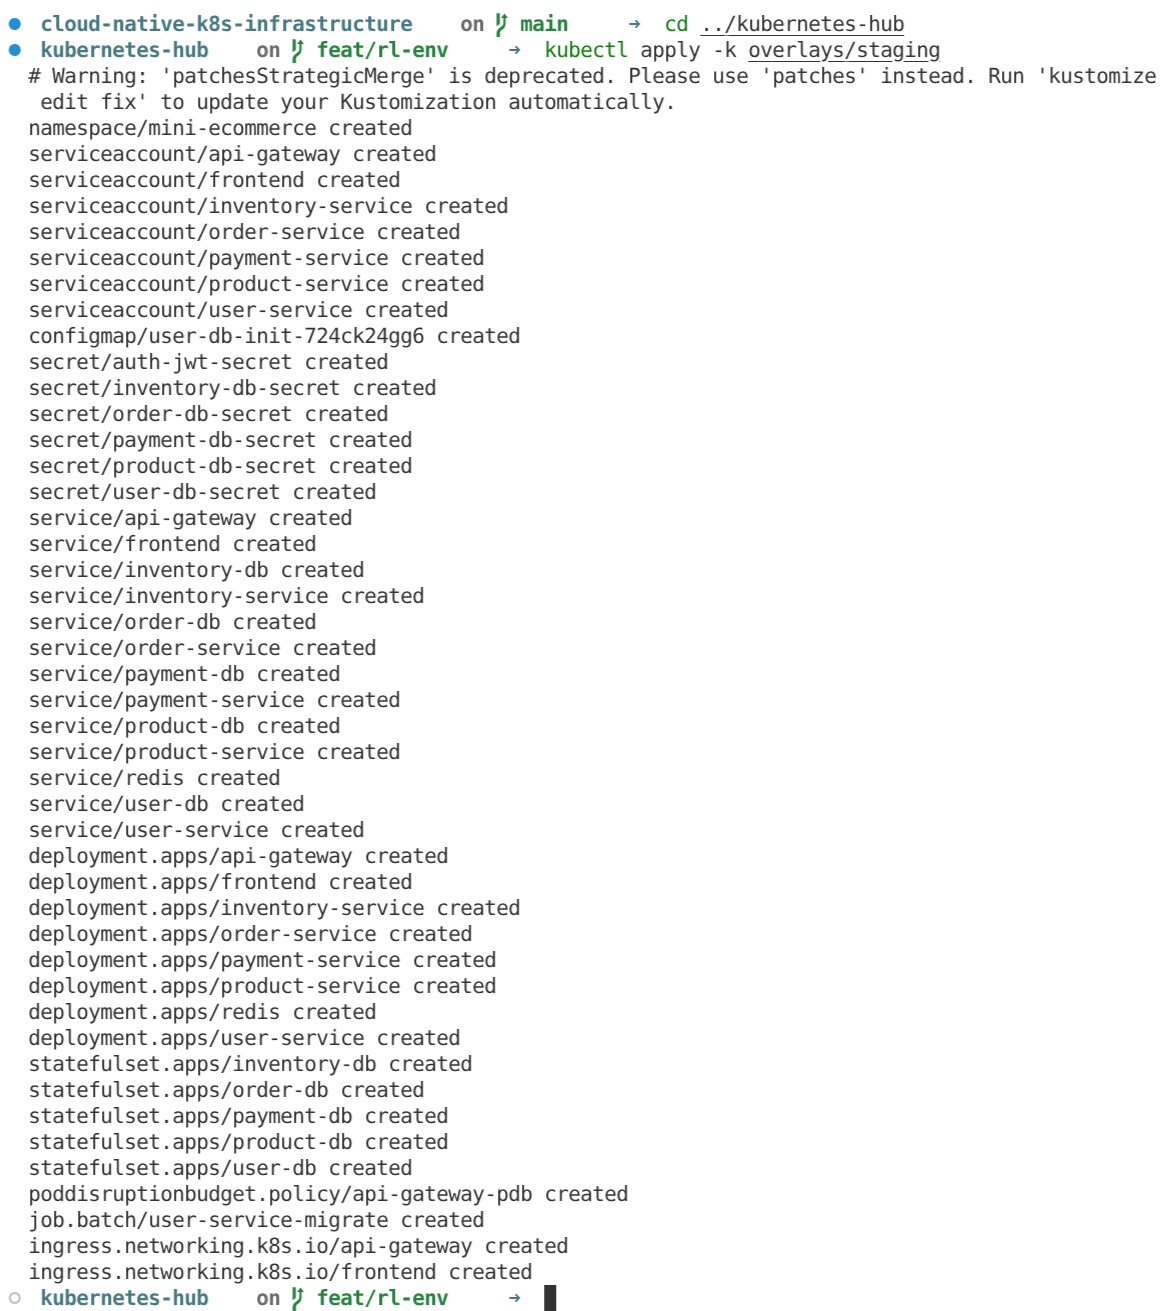
\includegraphics[width=0.95\textwidth]{graphics/chapter-5/5_4_application/deploy.png}
    \captionof{figure}{Triển khai bộ manifest ứng dụng microservices lên namespace \texttt{mini-ecommerce}}
    \label{fig:mini-ecommerce-deploy}
\end{center}

\noindent Ở mức triển khai, toàn bộ thành phần ứng dụng được đóng gói dưới dạng manifest Kubernetes và áp dụng bằng \texttt{kustomize} cho môi trường \texttt{staging}. Hình \ref{fig:mini-ecommerce-deploy} cho thấy quá trình \texttt{kubectl apply -k overlays/staging} đã khởi tạo đầy đủ namespace, service account, secret, service, deployment, statefulset, job migrate và ingress cần thiết. Cách tổ chức này giúp việc triển khai ứng dụng bám sát mô hình GitOps, đồng thời thuận tiện cho việc cập nhật cấu hình và tái lập thí nghiệm.

\begin{center}
    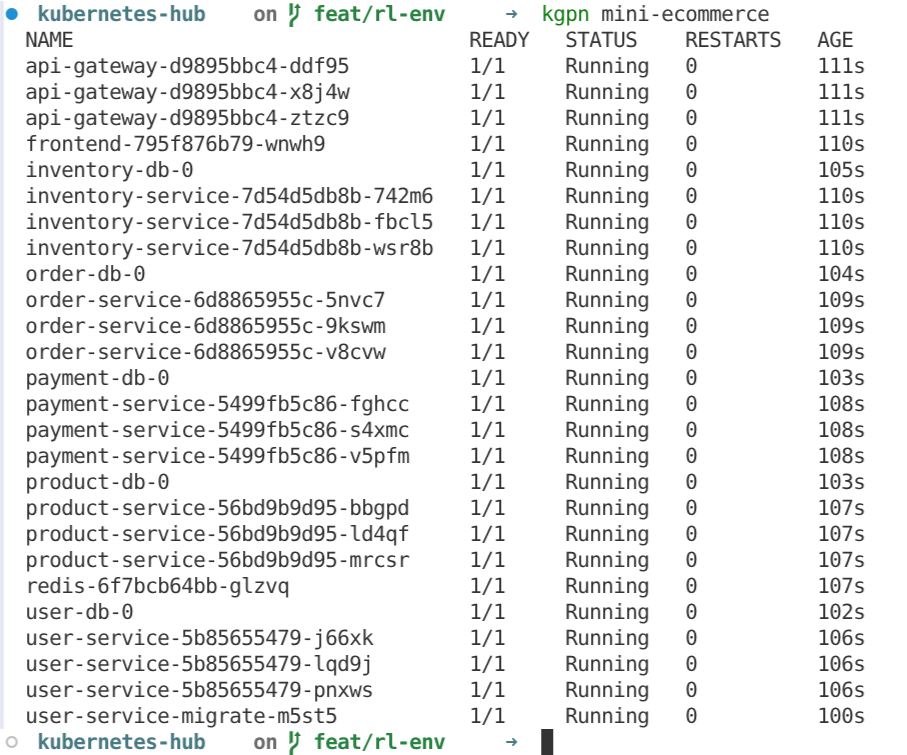
\includegraphics[width=0.7\textwidth]{graphics/chapter-5/5_4_application/get_pods.png}
    \captionof{figure}{Trạng thái Pod của ứng dụng sau khi triển khai lên Kubernetes}
    \label{fig:mini-ecommerce-pods}
\end{center}

\noindent Sau khi apply manifest, trạng thái runtime được kiểm tra nhanh bằng lệnh \texttt{kubectl get pods -n mini-ecommerce}. Hình \ref{fig:mini-ecommerce-pods} cho thấy các Pod của \texttt{api-gateway}, \texttt{frontend}, \texttt{user-service}, \texttt{product-service}, \texttt{inventory-service}, \texttt{payment-service}, \texttt{order-service}, \texttt{redis} và các cơ sở dữ liệu đều ở trạng thái \texttt{Running}. Đây là điều kiện cần để bước mô phỏng tải và mô phỏng sự cố ở các mục sau có thể diễn ra trên một môi trường dịch vụ hoàn chỉnh.

Về mặt thành phần, hệ thống runtime hiện tại gồm các dịch vụ chính:
\begin{itemize}
    \item \texttt{api-gateway}: điểm vào tập trung cho toàn bộ request từ phía người dùng.
    \item \texttt{user-service}: quản lý người dùng, xác thực và phân quyền.
    \item \texttt{product-service}: cung cấp chức năng quản lý và truy vấn sản phẩm.
    \item \texttt{inventory-service}: theo dõi, đặt giữ và hoàn trả tồn kho.
    \item \texttt{payment-service}: xử lý thanh toán và hoàn tiền khi cần bù trừ.
    \item \texttt{order-service}: điều phối quy trình tạo đơn hàng theo mô hình Saga.
    \item \texttt{front-end}: giao diện web phục vụ người dùng cuối.
    \item \texttt{Redis}: lớp trung gian bất đồng bộ cho trao đổi sự kiện giữa các service.
    \item \texttt{PostgreSQL}: hệ quản trị cơ sở dữ liệu được tách riêng theo từng miền nghiệp vụ.
\end{itemize}
\noindent Cách tổ chức này giúp hệ thống có đủ mức phân tán để quan sát các hiệu ứng lan truyền lỗi và hành vi phục hồi giữa nhiều thành phần.

\begin{center}
    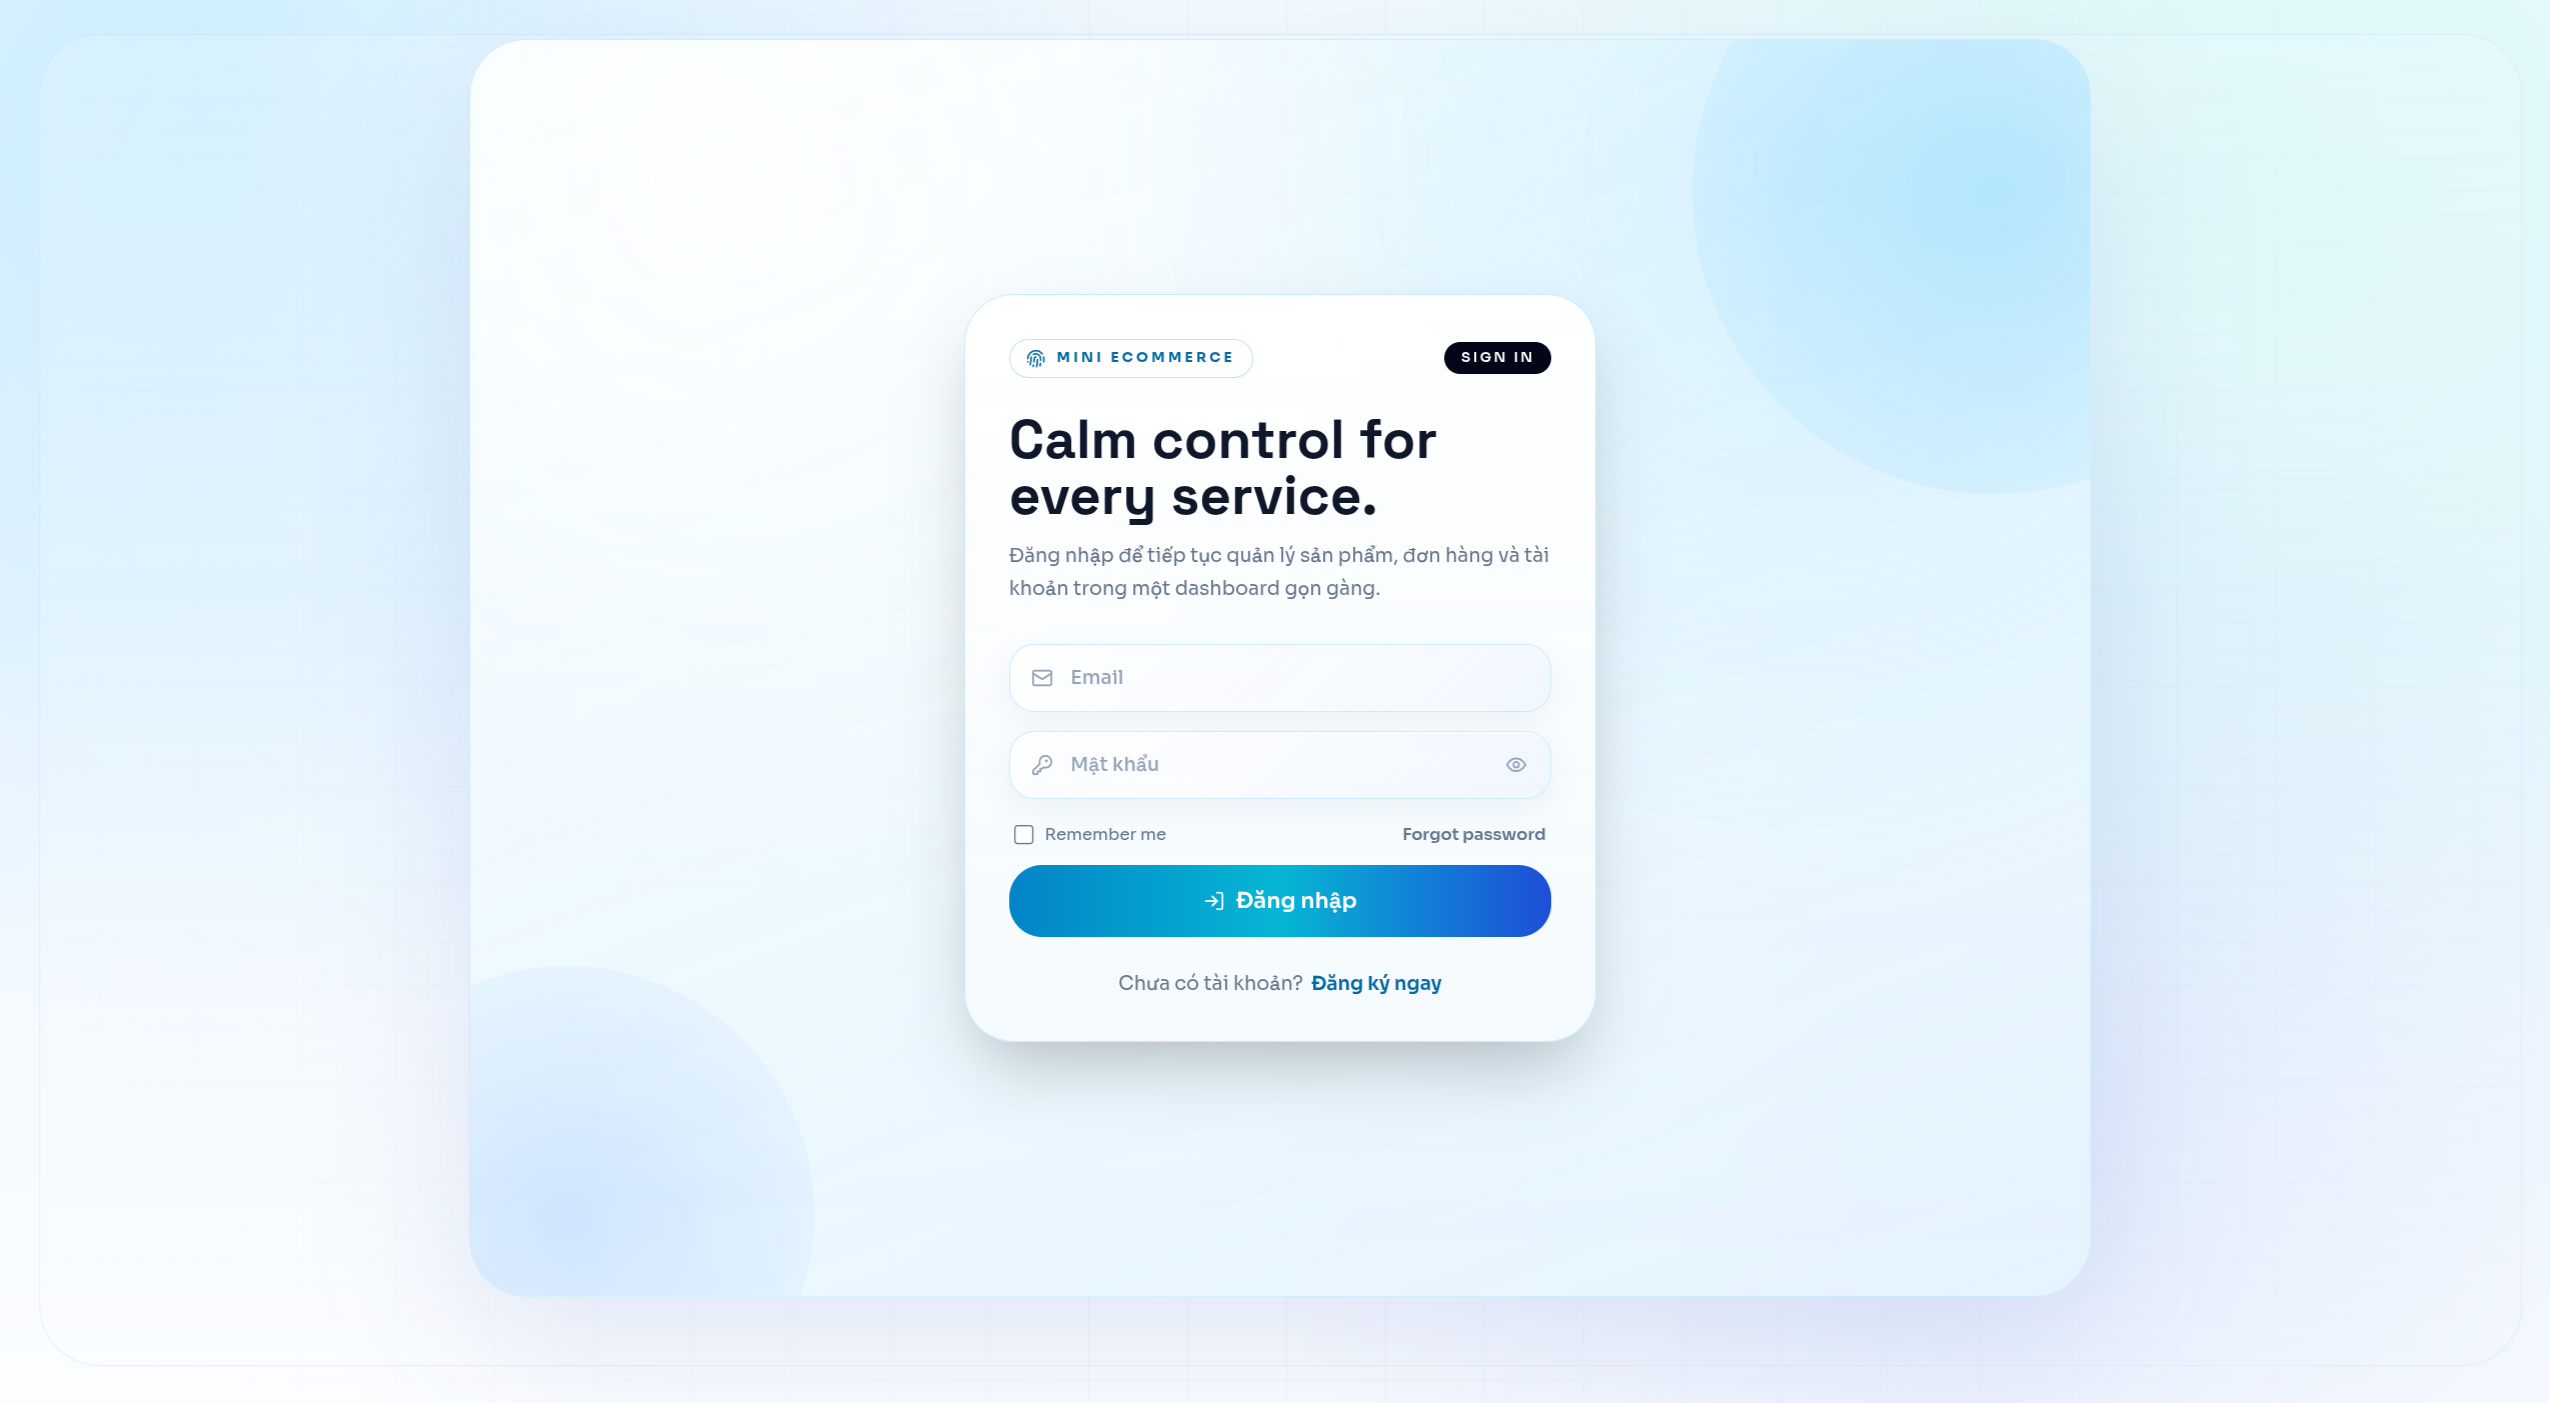
\includegraphics[width=0.98\textwidth]{graphics/chapter-5/5_4_application/login_register.png}
    \captionof{figure}{Giao diện đăng nhập của ứng dụng Mini Ecommerce}
    \label{fig:mini-ecommerce-login}
\end{center}

\noindent Ở phía người dùng cuối, ứng dụng cung cấp giao diện web để thao tác trực tiếp với các chức năng nghiệp vụ. Hình \ref{fig:mini-ecommerce-login} minh họa màn hình đăng nhập, nơi người dùng xác thực trước khi truy cập các chức năng quản trị sản phẩm, tồn kho và đơn hàng thông qua \texttt{api-gateway}.

\begin{center}
    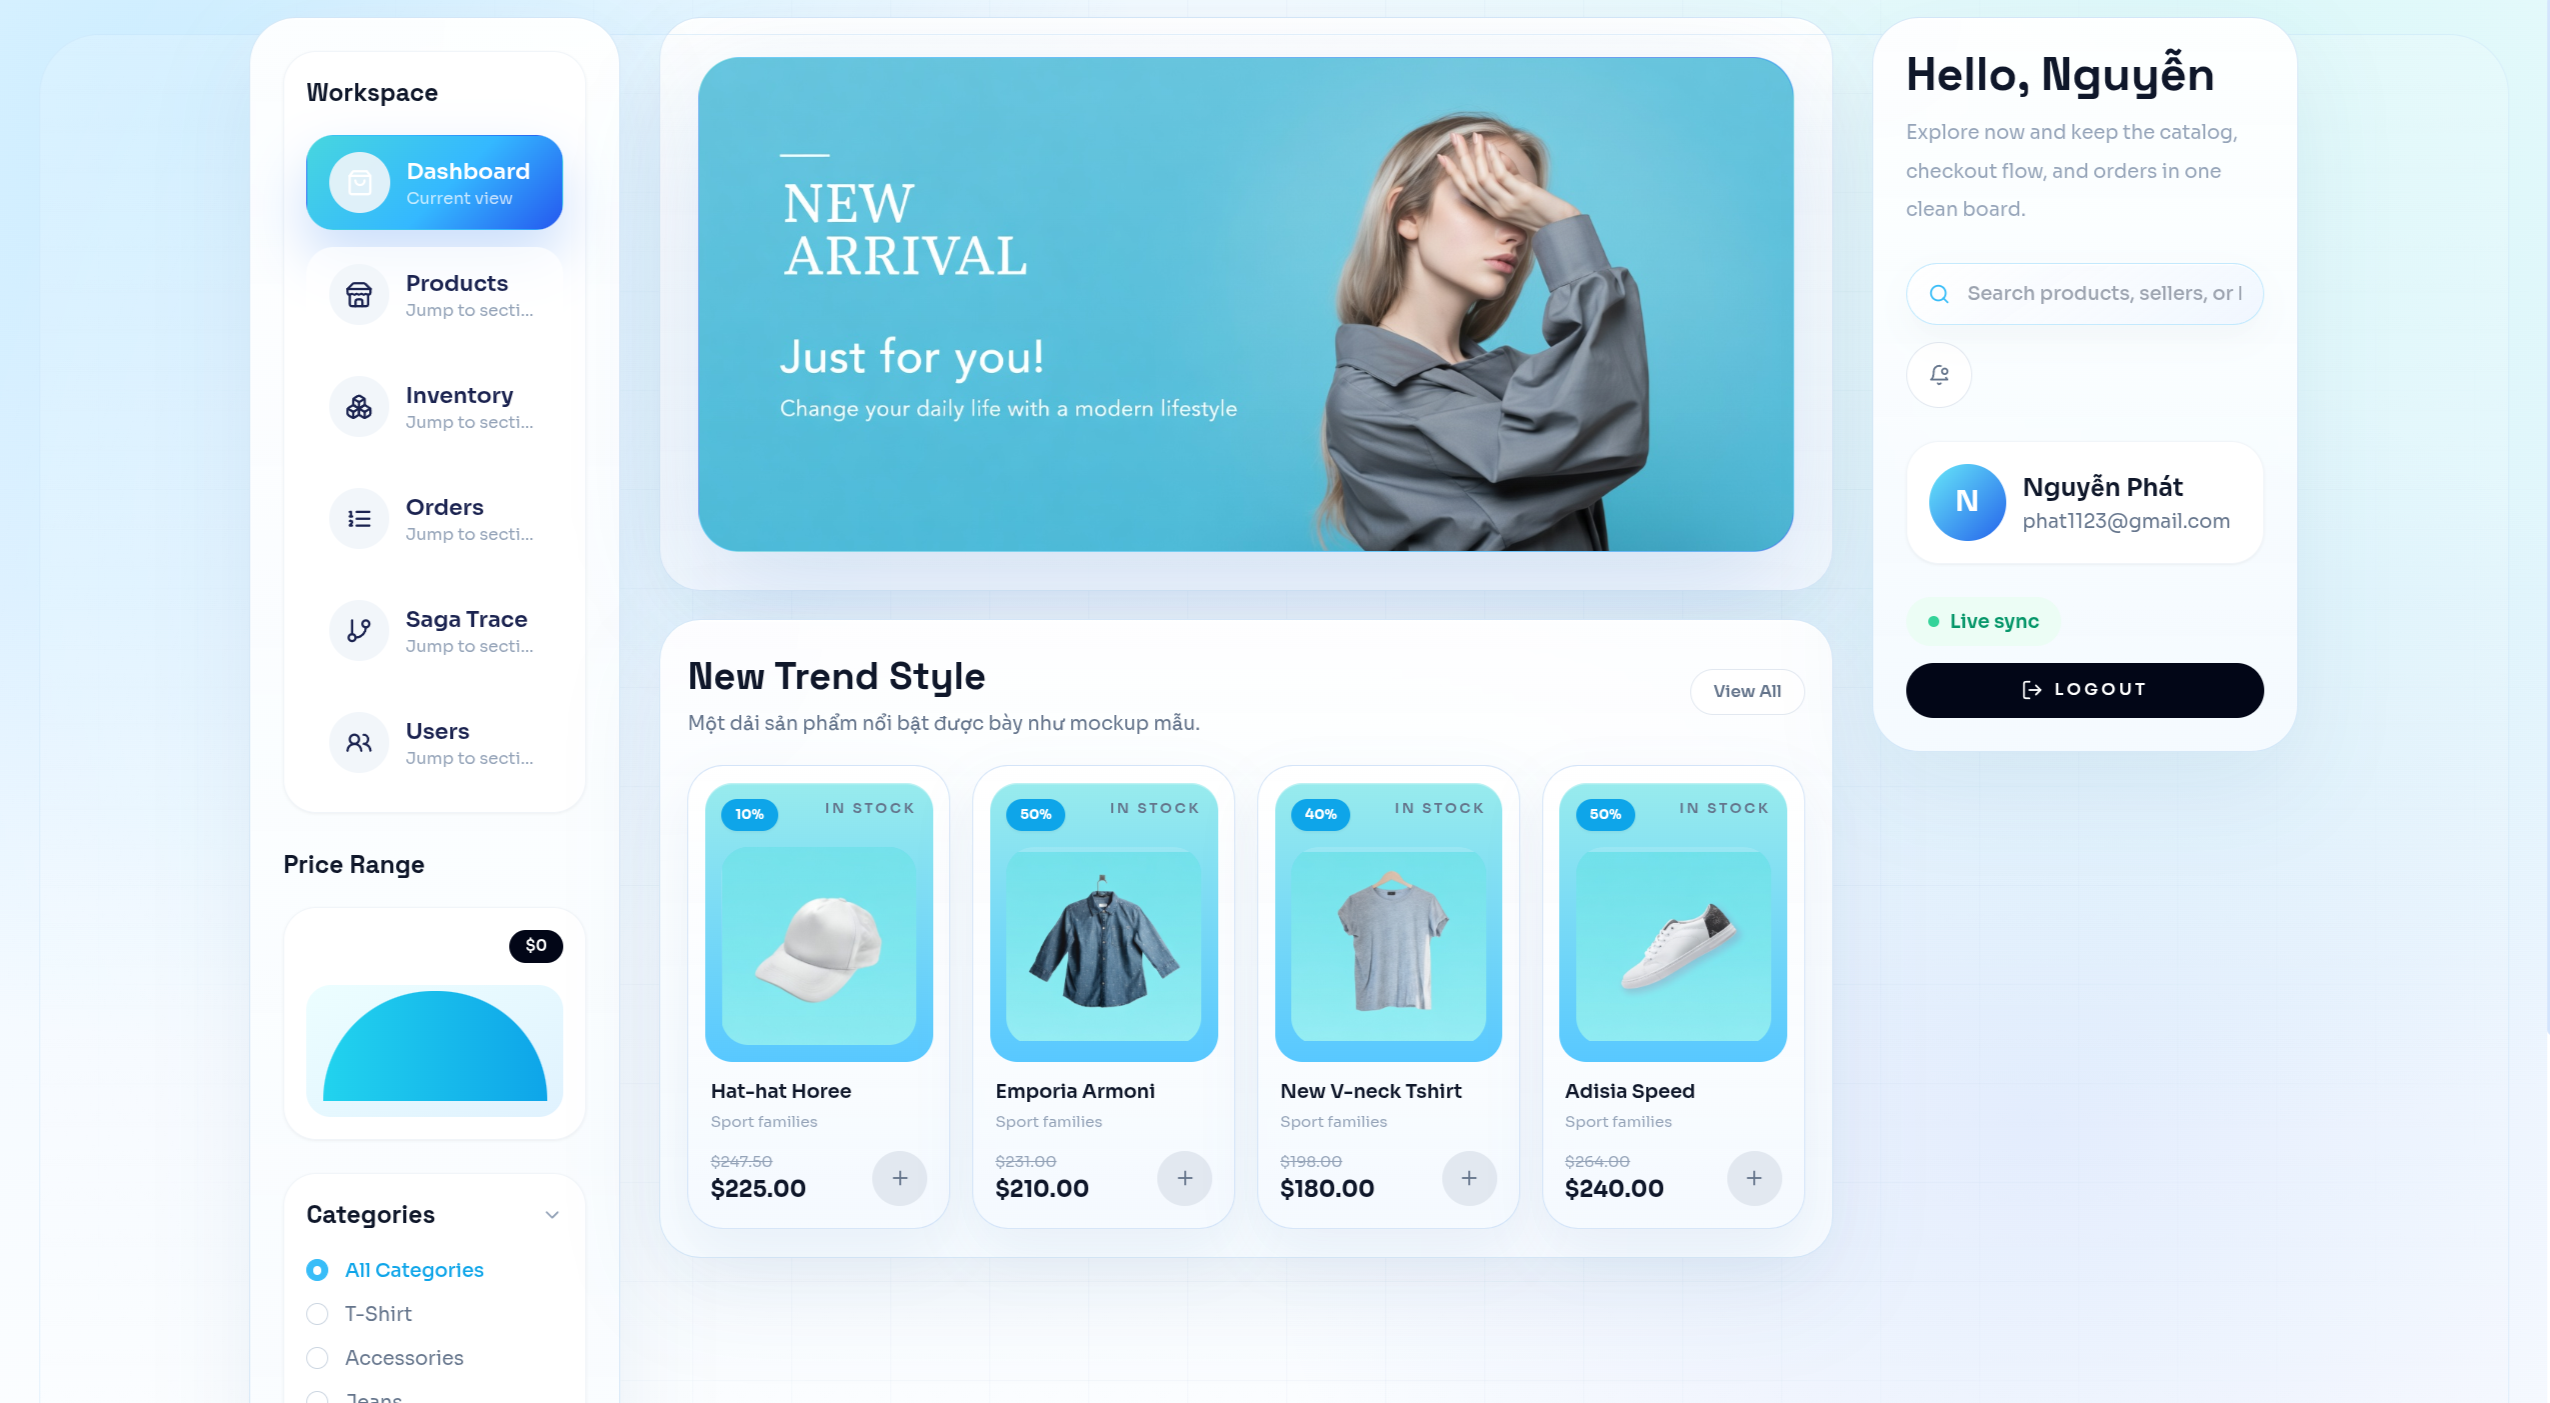
\includegraphics[width=0.98\textwidth]{graphics/chapter-5/5_4_application/main_ui.png}
    \captionof{figure}{Giao diện chính của hệ thống sau khi người dùng đăng nhập thành công}
    \label{fig:mini-ecommerce-main-ui}
\end{center}

\noindent Hình \ref{fig:mini-ecommerce-main-ui} cho thấy dashboard chính của ứng dụng với các khu vực chức năng như sản phẩm, tồn kho, đơn hàng, theo dõi saga và quản lý người dùng. Giao diện này là lớp tương tác trực tiếp để sinh ra các thao tác nghiệp vụ trong quá trình benchmark, từ đó tạo ra chuỗi request thực tế cho hệ thống microservices bên dưới.

Điểm quan trọng nhất của ứng dụng trong phạm vi đồ án là luồng xử lý đơn hàng theo mô hình \textit{Saga orchestration}. Khi một yêu cầu tạo đơn hàng được gửi tới \texttt{order-service}, hệ thống lần lượt thực hiện các bước đặt giữ tồn kho, xử lý thanh toán và cập nhật trạng thái đơn hàng; nếu một bước thất bại, cơ chế bù trừ sẽ được kích hoạt để hoàn tác các bước trước đó. Nhờ vậy, bài toán self-healing không chỉ dừng ở mức theo dõi tài nguyên hạ tầng mà còn gắn trực tiếp với chất lượng xử lý nghiệp vụ trong môi trường phân tán.

Ngoài các service nghiệp vụ, hệ thống còn tích hợp sẵn các thành phần giám sát được cài đặt cục bộ như \texttt{Prometheus}, \texttt{Grafana}, \texttt{Loki} và \texttt{Tempo}. Điều này tạo điều kiện thu thập đồng thời chỉ số hạ tầng, chỉ số ứng dụng và dấu vết truy vết phân tán, từ đó hình thành tập trạng thái đầu vào cho tác nhân RL. Vì vậy, \textit{Mini Ecommerce Microservices} vừa đóng vai trò hệ thống mục tiêu để triển khai self-healing, vừa là nguồn sinh dữ liệu thực nghiệm cho các bước huấn luyện và đánh giá ở các mục sau.

\section{Mô phỏng hoạt động thực tế của hệ thống}

\subsection{Mô phỏng lượng người dùng sử dụng K6}

Trong thực nghiệm, K6 được sử dụng để mô phỏng tải người dùng lên hệ thống \textit{mini-ecommerce} thông qua kịch bản \texttt{scripts-k6/user-journey.js}. Kịch bản bám theo luồng truy cập thực tế: đăng nhập, duyệt danh mục sản phẩm, xem chi tiết sản phẩm và truy vấn đơn hàng. Cách mô phỏng này giúp dữ liệu tải phản ánh sát hành vi nghiệp vụ thay vì chỉ gửi request tổng hợp.

Quá trình chạy được điều phối bởi script \texttt{scripts/run-user-journey.sh}. Script này tự động nạp cấu hình từ tệp môi trường, seed dữ liệu khách hàng/sản phẩm trước khi chạy (nếu bật), thực thi K6, sau đó dọn dẹp dữ liệu seed để tránh ảnh hưởng lần thử nghiệm kế tiếp. Nhờ đó, các lượt chạy có tính lặp lại cao và thuận tiện so sánh giữa nhiều kịch bản chaos.

\begin{center}
    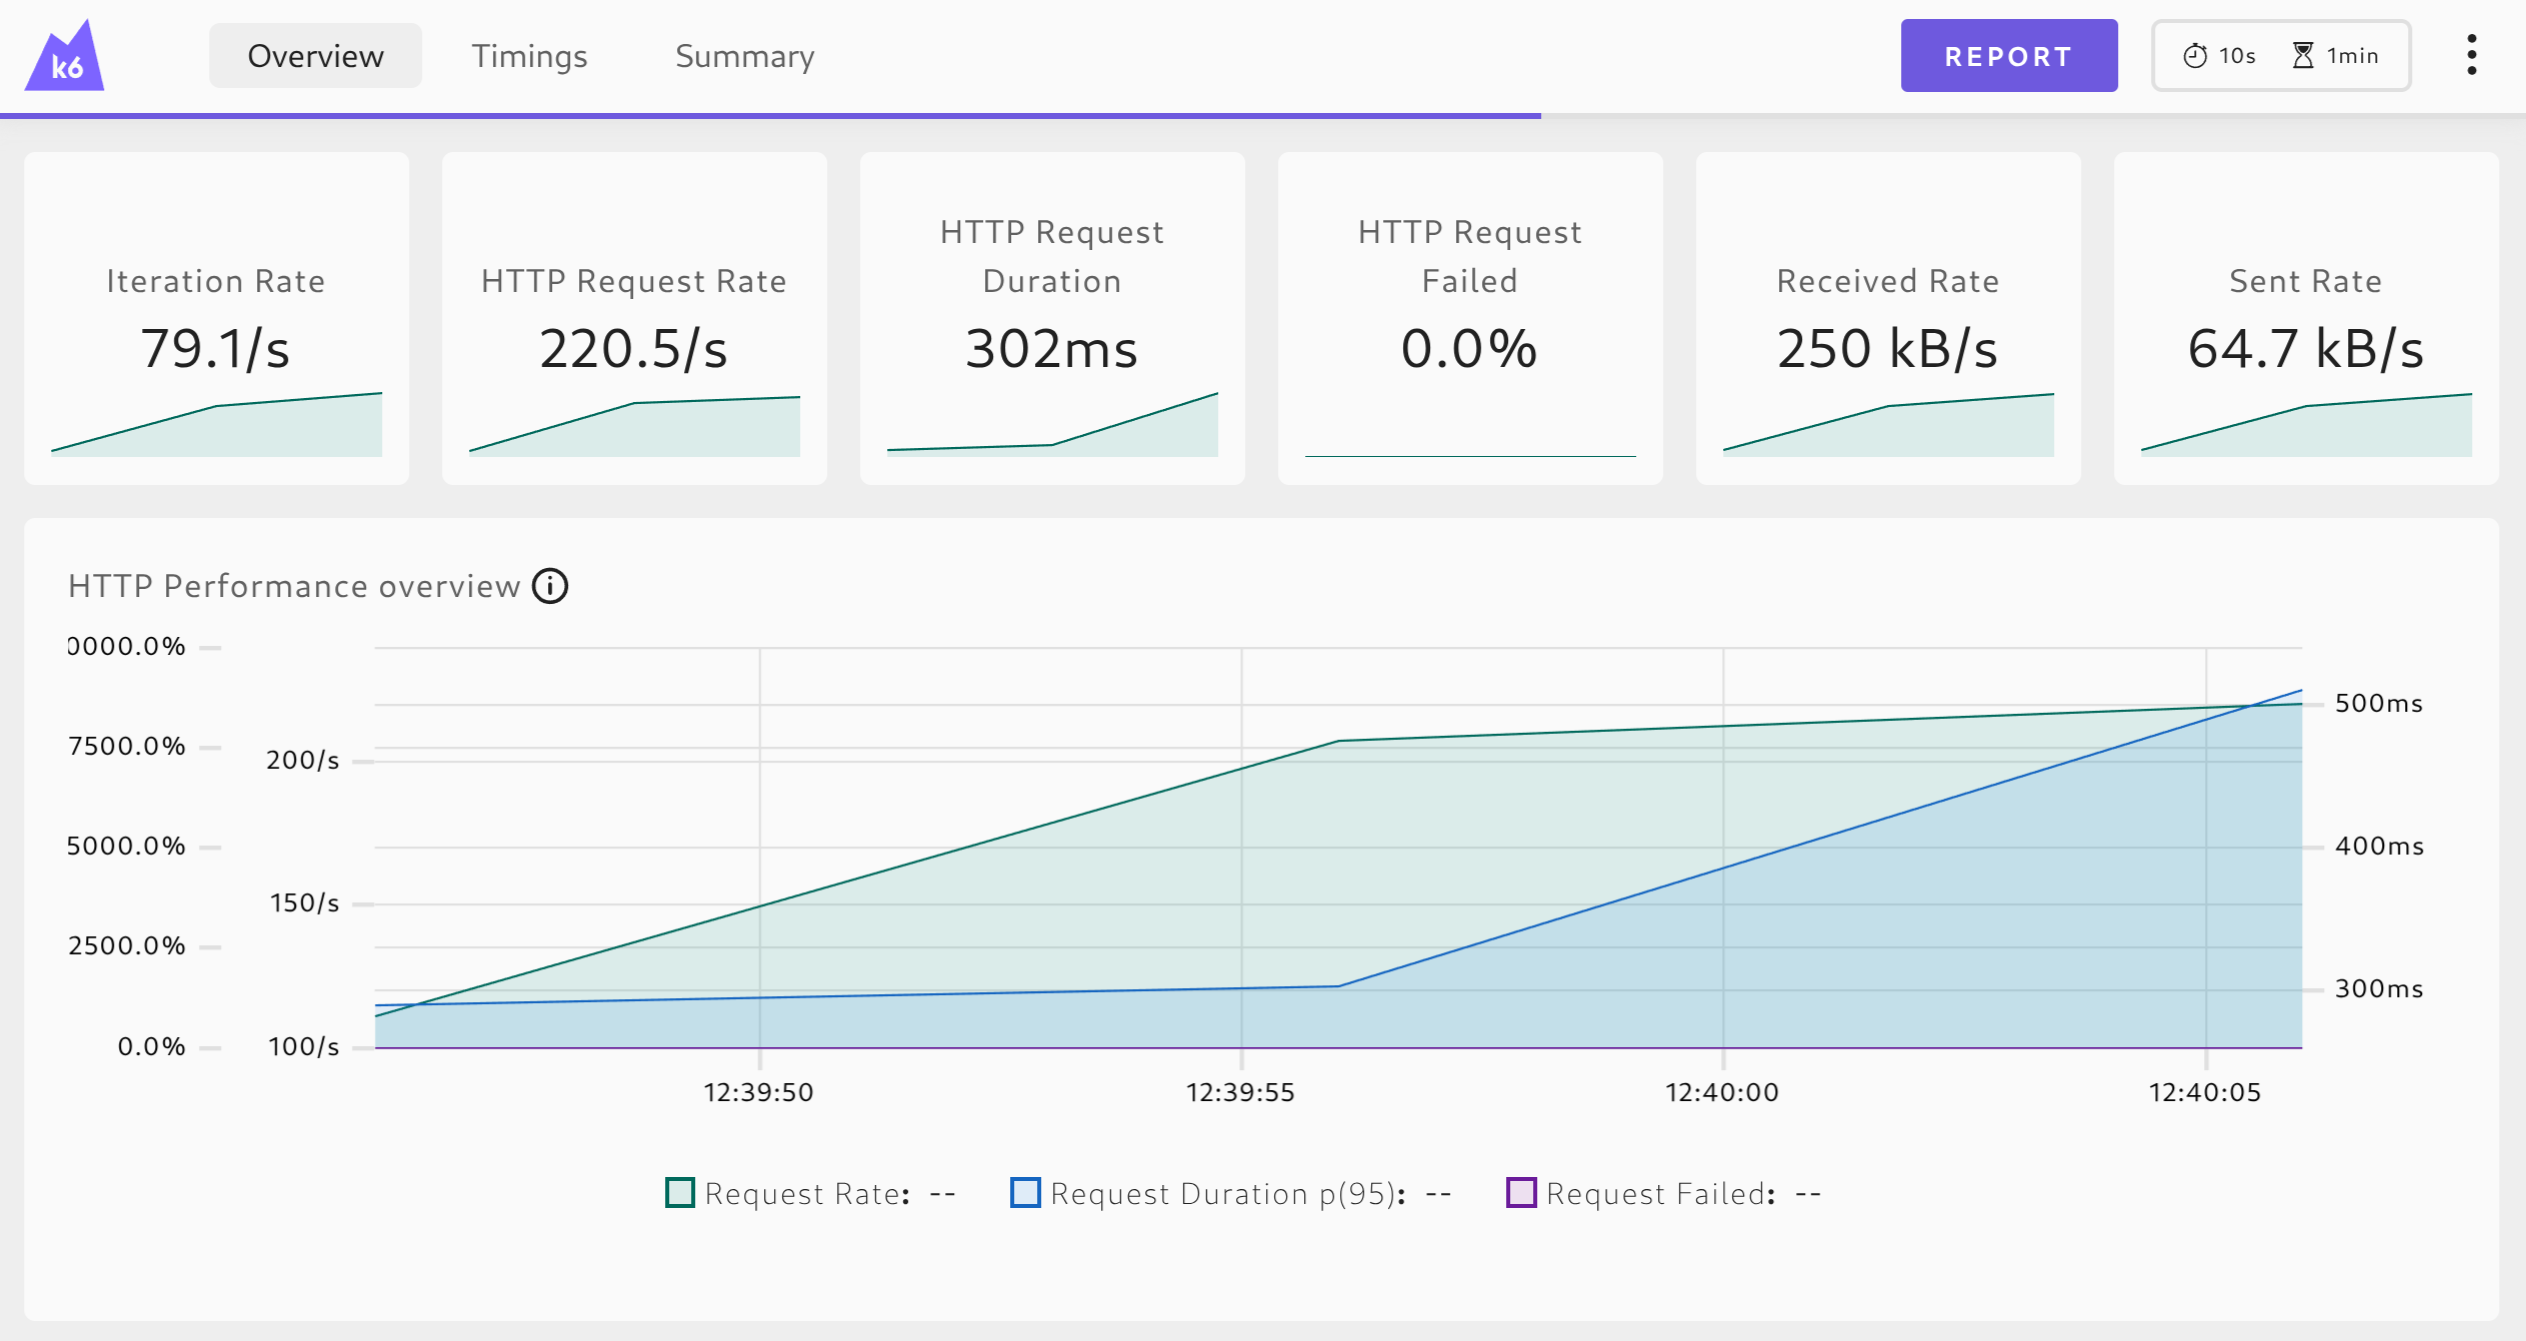
\includegraphics[width=0.98\textwidth]{graphics/chapter-5/5_5_k6/k6_overview.png}
    \captionof{figure}{Tổng quan dashboard K6 của một lượt chạy mô phỏng tải người dùng}
    \label{fig:k6-overview}
\end{center}

\noindent Hình \ref{fig:k6-overview} cho thấy dashboard tổng quan của K6 sau khi kết thúc một lượt benchmark. Các chỉ số ở phần đầu màn hình phản ánh mức tải quan sát được trong lượt chạy, gồm \textit{iteration rate}, \textit{HTTP request rate}, độ trễ HTTP và tỷ lệ request thất bại. Ở hình này, hệ thống vẫn duy trì \texttt{0.0\%} request lỗi trong khi thông lượng và độ trễ đã bắt đầu tăng theo mức tải.

\begin{center}
    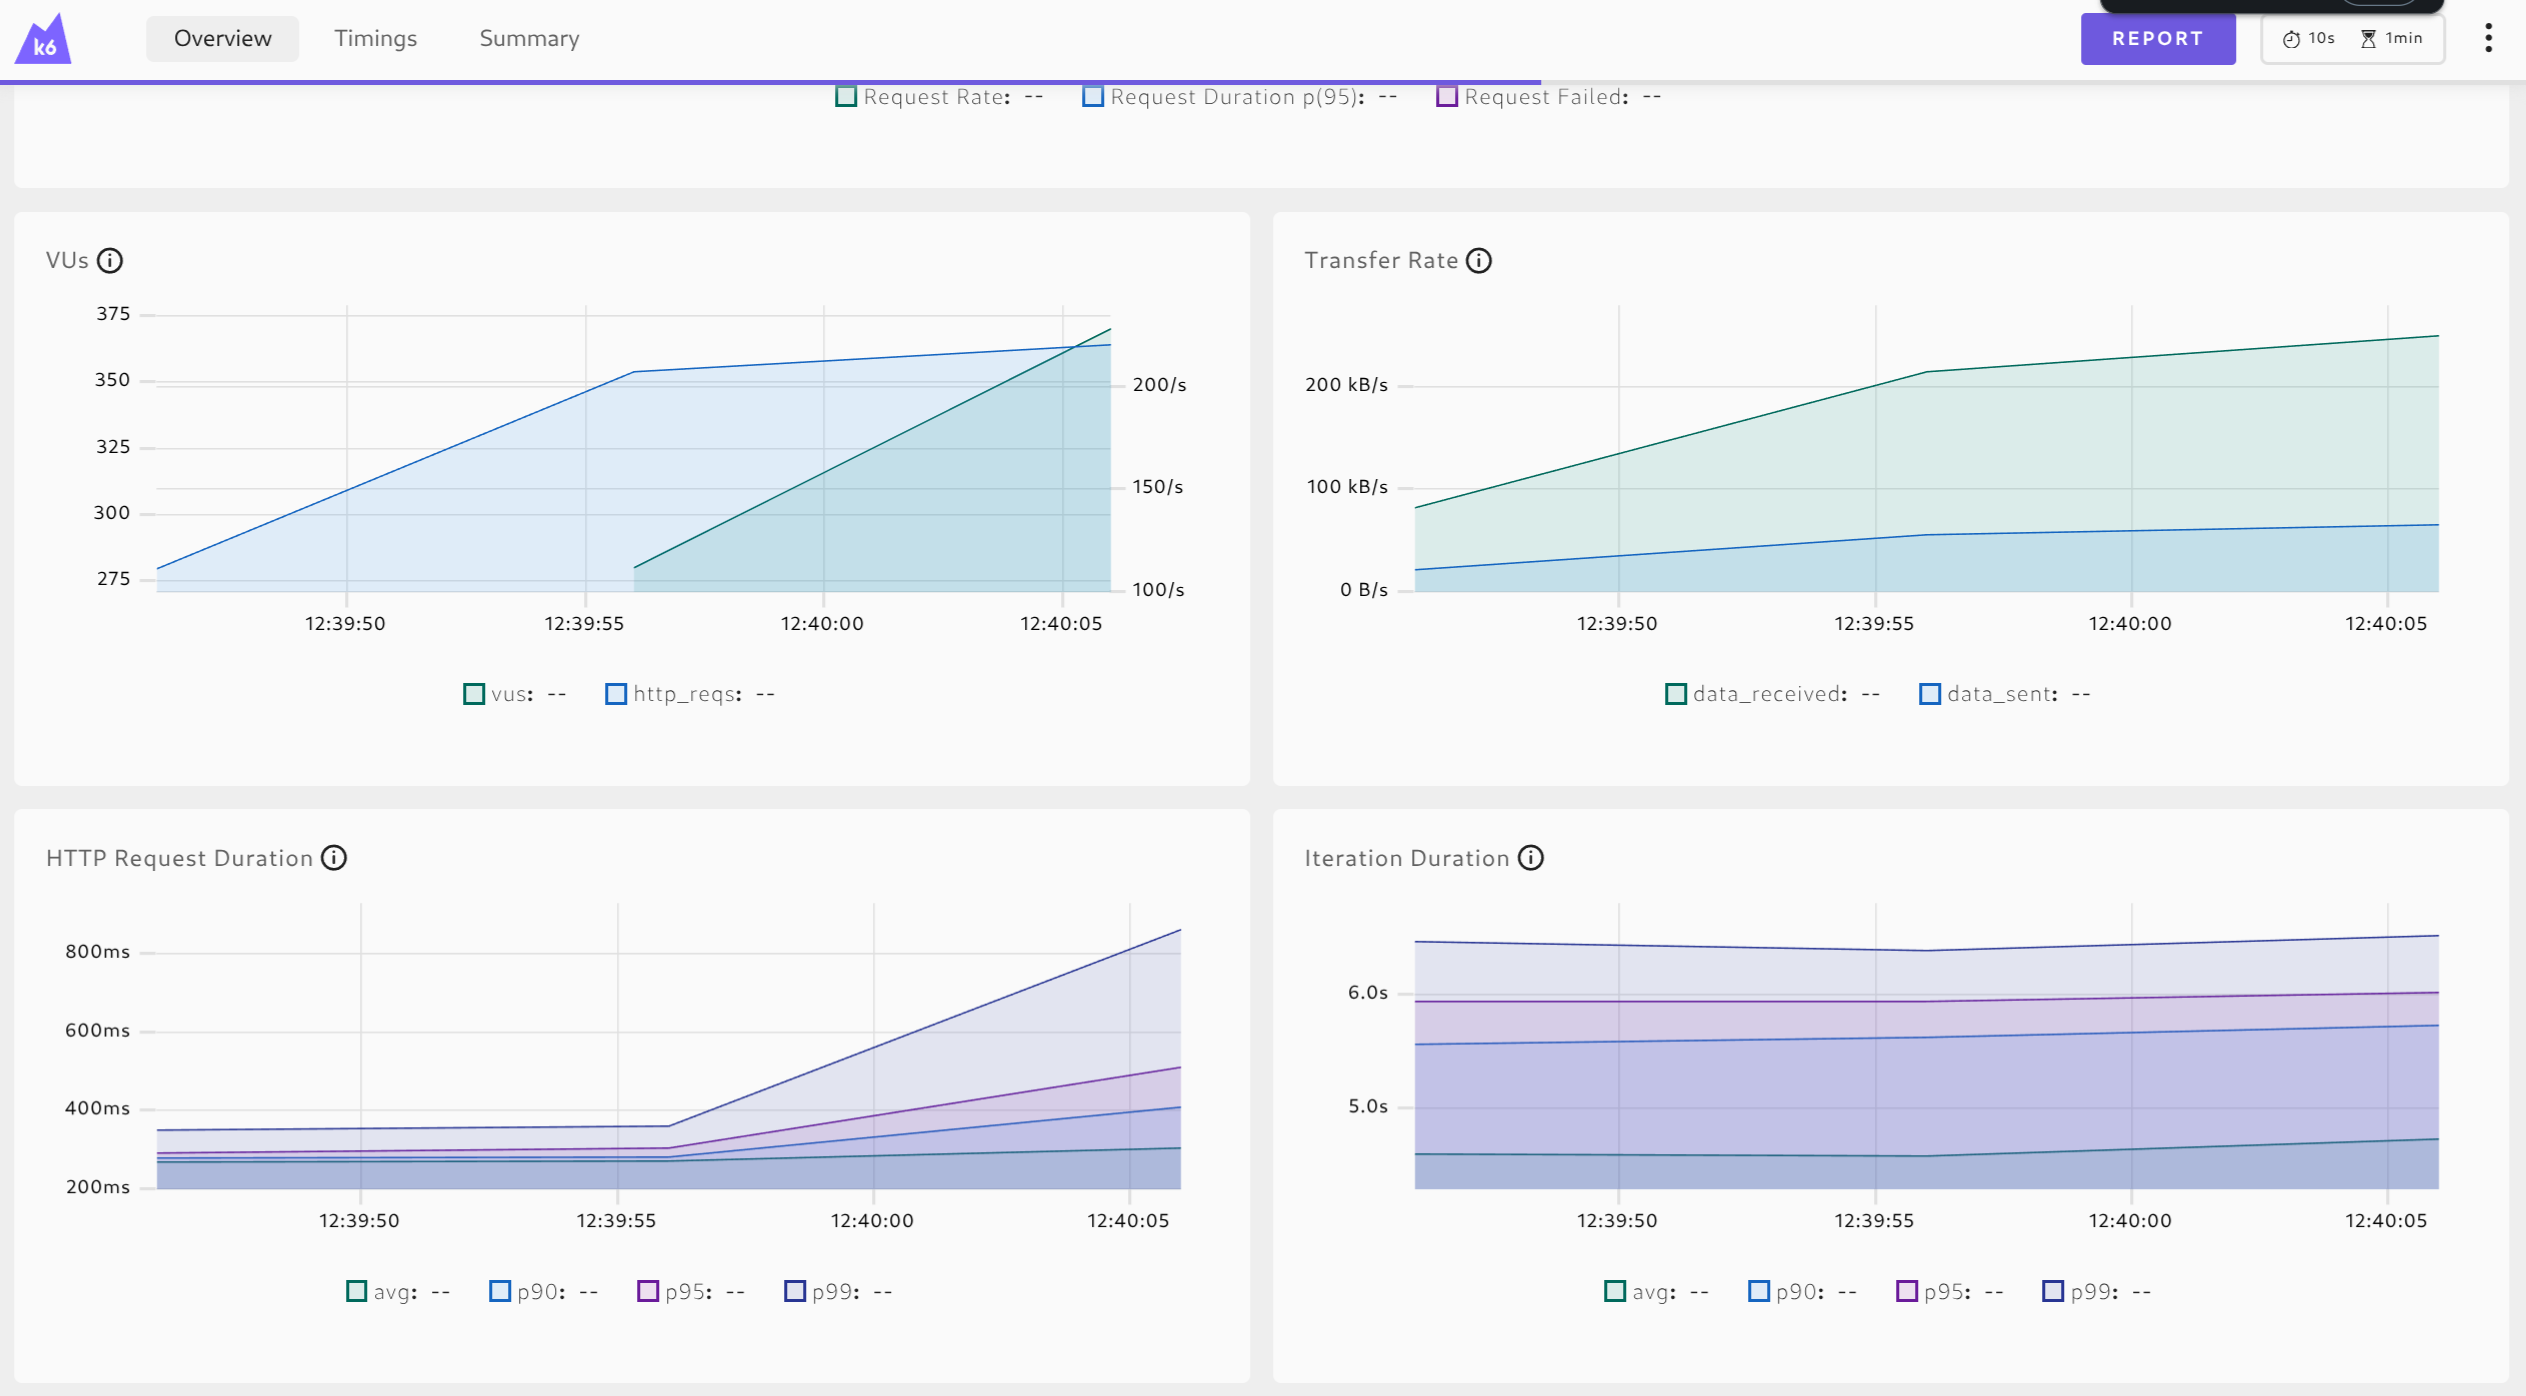
\includegraphics[width=0.98\textwidth]{graphics/chapter-5/5_5_k6/k6_performance_charts.png}
    \captionof{figure}{Biểu đồ tải, thông lượng và độ trễ trong lượt chạy K6}
    \label{fig:k6-performance-charts}
\end{center}

\noindent Hình \ref{fig:k6-performance-charts} thể hiện rõ quá trình tăng tải theo từng bước. Số lượng \textit{virtual users} tăng dần kéo theo \textit{HTTP request rate} và \textit{transfer rate} tăng tương ứng, trong khi độ trễ \textit{p95/p99} cũng tăng dần về cuối lượt chạy. Điều này cho thấy kịch bản K6 đã tạo ra đủ áp lực để quan sát phản ứng của hệ thống ở các mức tải khác nhau.

\begin{center}
    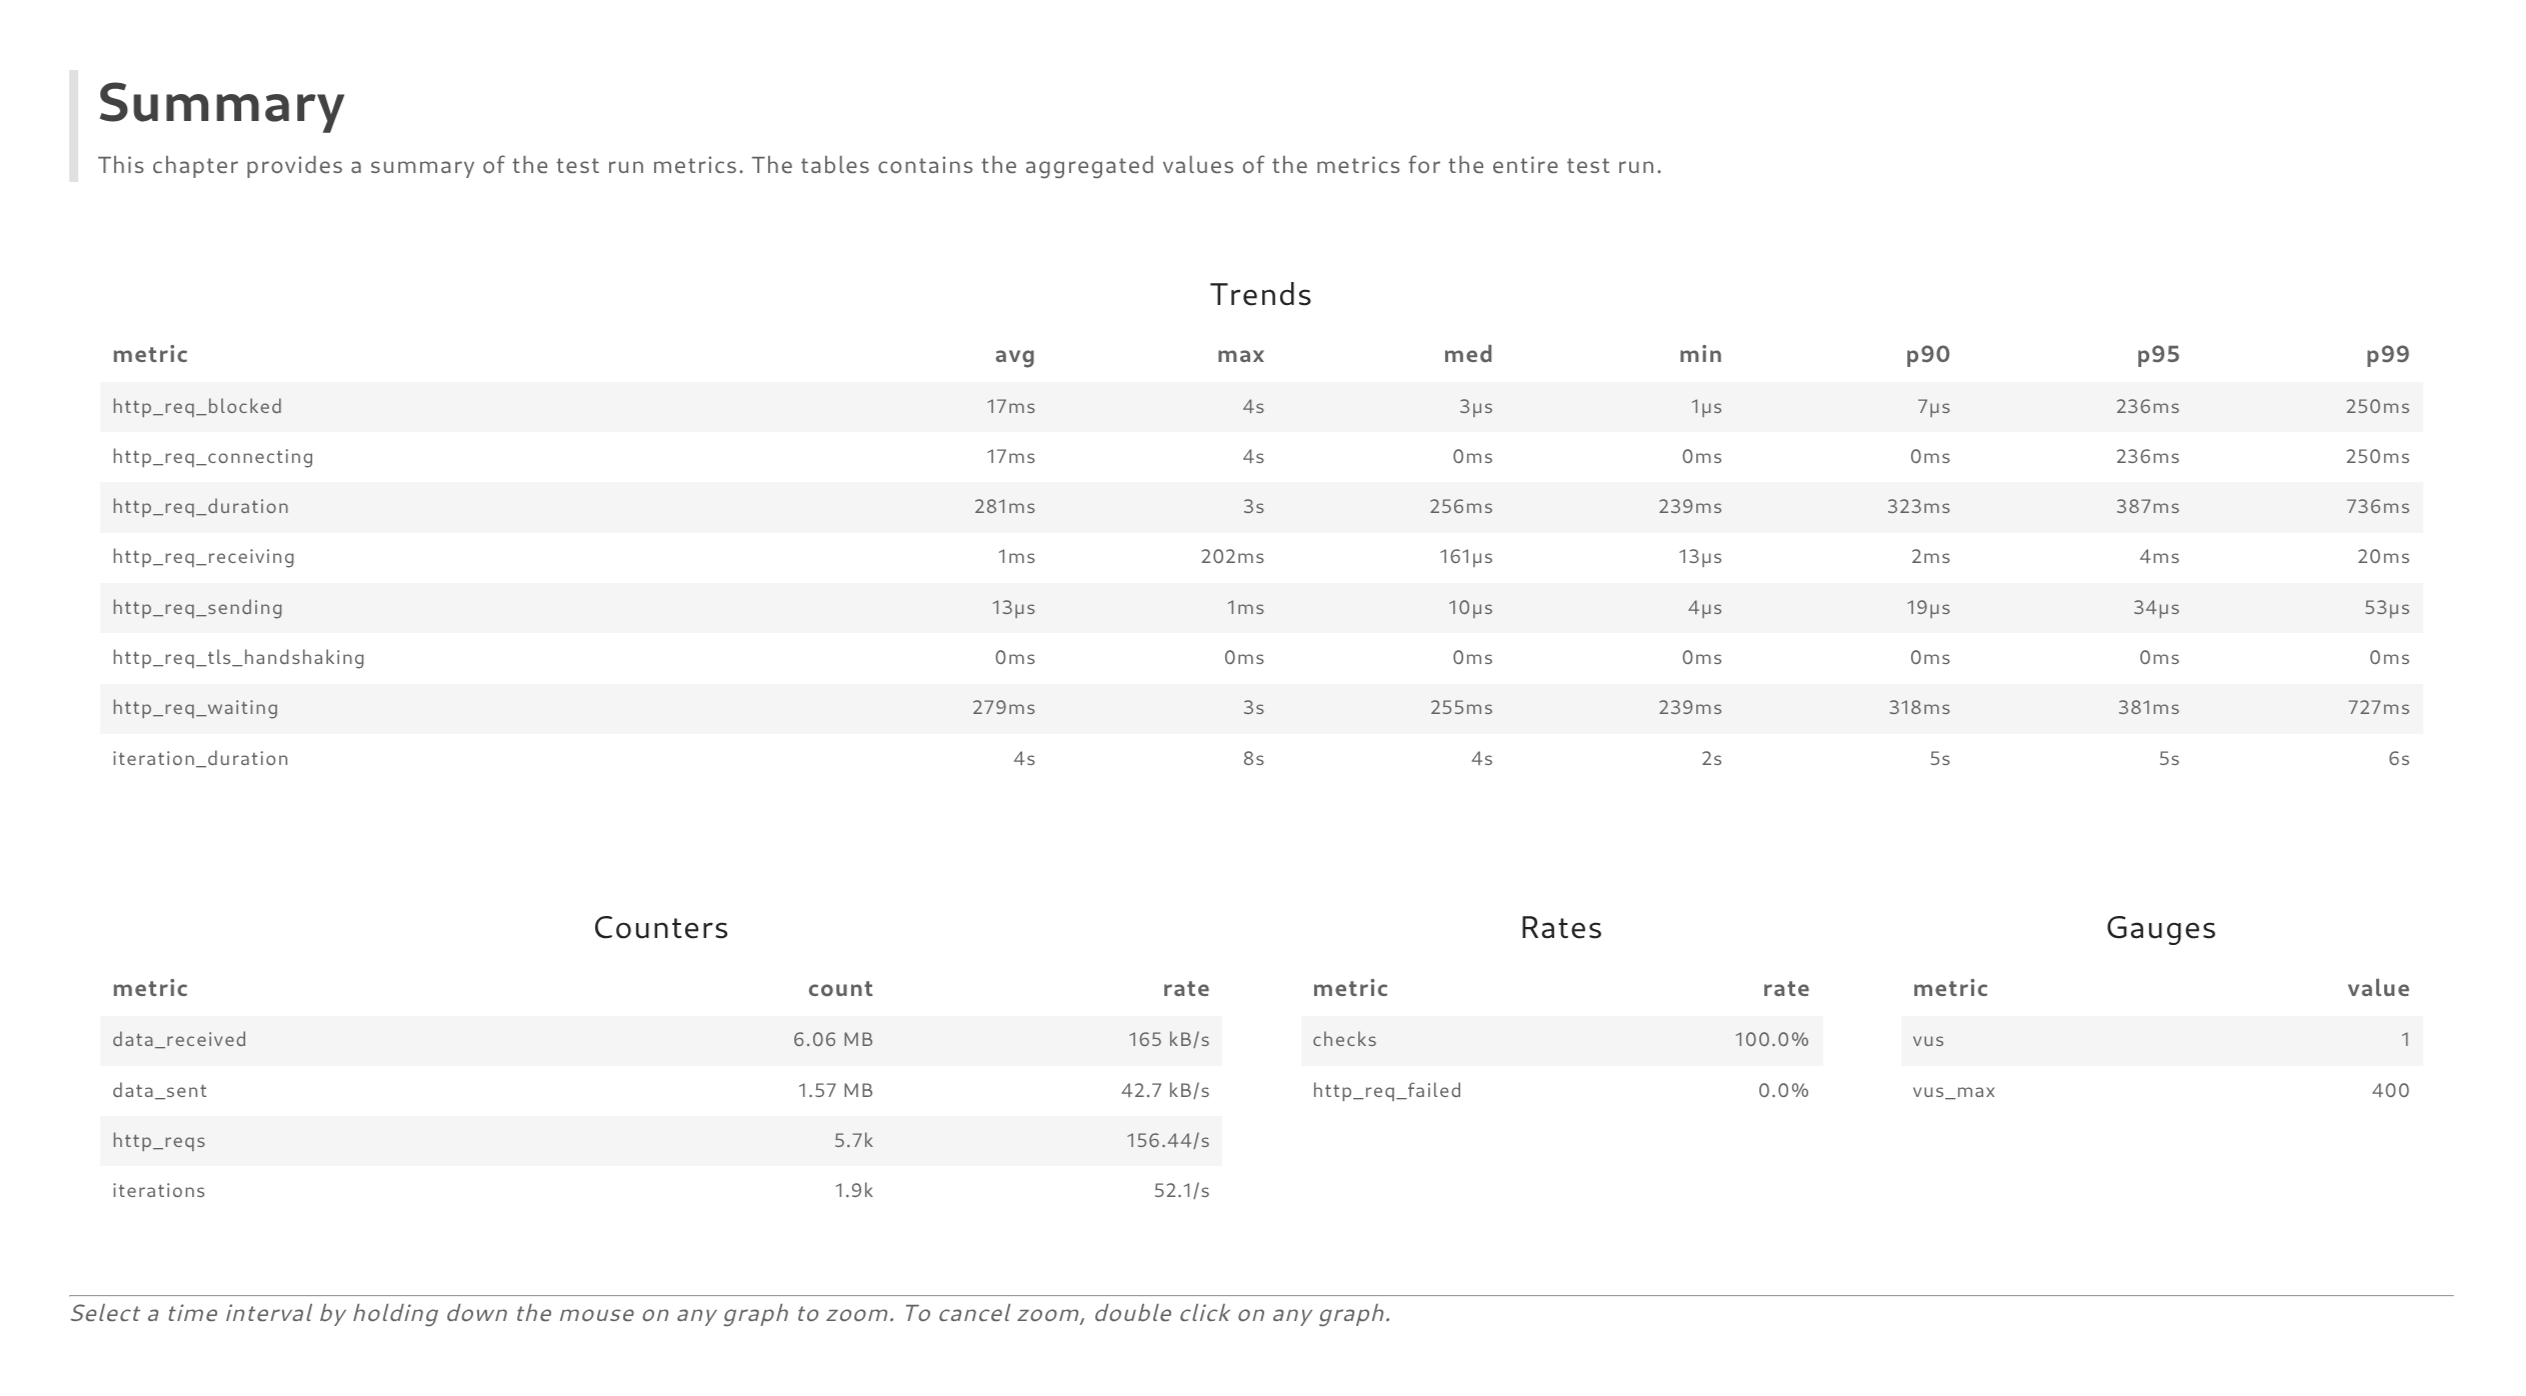
\includegraphics[width=0.98\textwidth]{graphics/chapter-5/5_5_k6/k6_summary_table.png}
    \captionof{figure}{Bảng Summary của K6 sau khi hoàn tất benchmark}
    \label{fig:k6-summary-table}
\end{center}

\noindent Hình \ref{fig:k6-summary-table} tổng hợp các thống kê sau khi chạy xong benchmark. Trong lượt chạy này, \texttt{http\_req\_duration} trung bình vào khoảng \texttt{281ms}, \texttt{p95} đạt \texttt{387ms}, \texttt{p99} lên tới \texttt{736ms} và tỷ lệ lỗi vẫn giữ ở mức \texttt{0.0\%}. Các số liệu này đủ để làm đường cơ sở khi so sánh với những lần chạy có tiêm lỗi ở các phần sau.

\begin{center}
    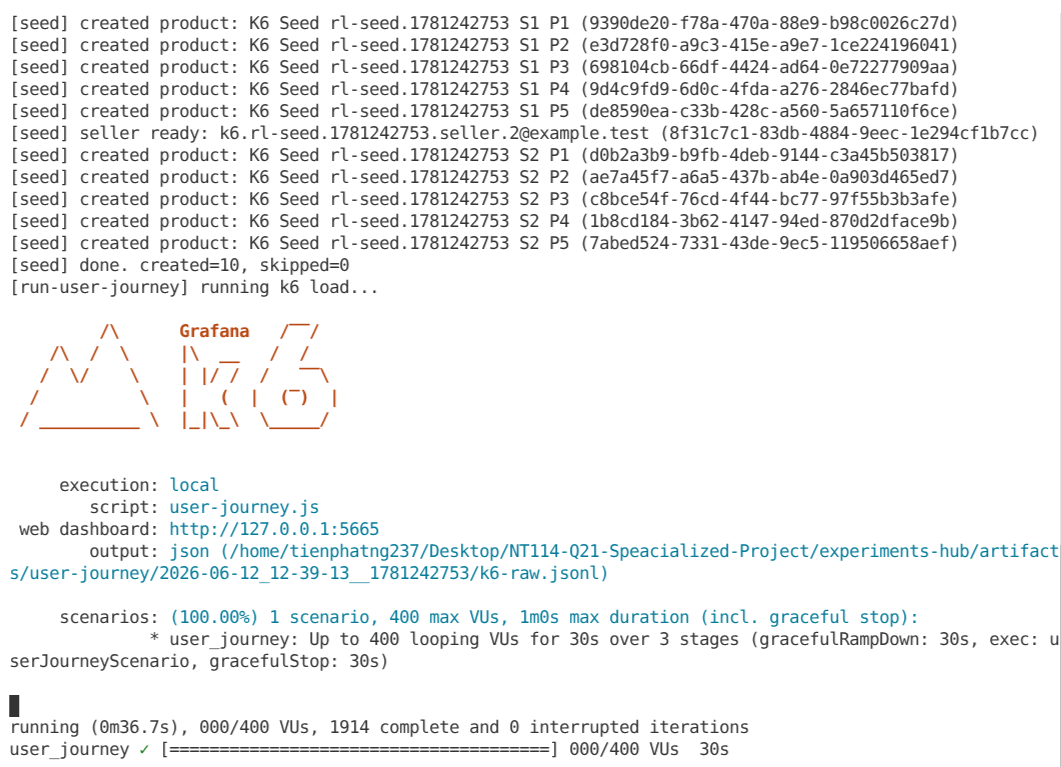
\includegraphics[width=0.98\textwidth]{graphics/chapter-5/5_5_k6/k6_run_log.png}
    \captionof{figure}{Nhật ký thực thi kịch bản K6 và xuất dữ liệu kết quả}
    \label{fig:k6-run-log}
\end{center}

\noindent Hình \ref{fig:k6-run-log} cho thấy quá trình khởi chạy kịch bản, sinh dữ liệu seed và ghi kết quả đầu ra. Sau khi K6 kết thúc, hệ thống xuất dữ liệu thô và dữ liệu tổng hợp theo các mốc thời gian:
\begin{itemize}
    \item \texttt{k6-summary.json}
    \item \texttt{k6-raw.jsonl}
    \item \texttt{combined-report.json}
    \item \texttt{combined-report.csv}
    \item \texttt{combined-report.parquet}
\end{itemize}
\noindent Đặc biệt, bước \texttt{export-combined-report.py} sẽ hợp nhất chỉ số K6 với dữ liệu Prometheus theo bucket 5 giây, tạo thành tập dữ liệu đầu vào trực tiếp cho phân tích hiệu năng và huấn luyện tác nhân RL.

\begin{center}
\captionof{table}{Một số thông số chính trong cấu hình K6 (\texttt{.env.k6.fast})}
\label{tab:k6-fast-profile-config}
\footnotesize
\renewcommand{\arraystretch}{1.0}
\begin{tabular}{|L{4.0cm}|C{3.0cm}|L{7.6cm}|}
\hline
\textbf{Tham số} & \textbf{Giá trị} & \textbf{Ý nghĩa} \\ \hline
\texttt{BASE\_URL} & \texttt{ALB DNS của hệ thống staging} & Địa chỉ endpoint mục tiêu để phát sinh tải thử nghiệm. \\ \hline
\makecell[l]{\texttt{LOGIN\_ENDPOINT}\\\texttt{PRODUCTS\_ENDPOINT}\\\texttt{ORDERS\_ENDPOINT}} & \texttt{/api/v1/...} & Các API chính trong luồng mô phỏng người dùng. \\ \hline
\texttt{VU\_START} & \texttt{100} & Số lượng người dùng ảo ban đầu. \\ \hline
\texttt{VU\_MAX} & \texttt{250} & Mức người dùng ảo cực đại trong profile tải nhanh. \\ \hline
\texttt{VU\_STEP} & \texttt{15} & Bước tăng người dùng ảo theo mỗi chu kỳ tải. \\ \hline
\texttt{VU\_TIME\_UNIT} & \texttt{10s} & Đơn vị thời gian cho mỗi bước tăng tải. \\ \hline
\makecell[l]{\texttt{VU\_RAMP\_DOWN}\\\texttt{\_DURATION}} & \texttt{10s} & Thời gian giảm tải có kiểm soát trước khi kết thúc lượt chạy. \\ \hline
\texttt{CUSTOMER\_COUNT} & \texttt{5} & Số lượng tài khoản khách hàng được sinh sẵn cho mỗi lần test. \\ \hline
\texttt{THINK\_TIME\_MIN/MAX} & \texttt{0.5 / 2.0} & Khoảng thời gian chờ mô phỏng hành vi người dùng giữa các thao tác. \\ \hline
\texttt{REQUEST\_TIMEOUT} & \texttt{30s} & Ngưỡng timeout cho mỗi HTTP request trong kịch bản K6. \\ \hline
\texttt{PROMETHEUS\_URL} & \texttt{10.0.21.10} & IP của Prometheus Server dùng để thu thập metrics cho đánh giá/huấn luyện RL. \\ \hline
\end{tabular}
\end{center}

\subsection{Mô phỏng sự cố trong quá trình sử dụng}

Để đánh giá khả năng tự phục hồi trong điều kiện vận hành thực, Chaos Mesh được sử dụng để tiêm lỗi trong lúc hệ thống đang phục vụ tải từ K6. Quá trình này được điều phối bởi script \texttt{chaos-mesh/scripts/run-chaos.sh}, cho phép chuẩn hóa cùng một quy trình giữa các lần chạy và giữa các loại sự cố khác nhau.

Mỗi lượt thí nghiệm được tổ chức theo 4 pha thời gian:
\begin{itemize}
    \item \textbf{Baseline}: hệ thống chạy ổn định dưới tải.
    \item \textbf{Warm-up}: tăng độ ổn định của tín hiệu trước khi kích hoạt lỗi.
    \item \textbf{Chaos-active}: lỗi được tiêm trực tiếp bằng manifest Chaos Mesh.
    \item \textbf{Recovery}: ngừng tiêm lỗi và quan sát hệ thống phục hồi.
\end{itemize}
\noindent Theo cấu hình hiện tại trong \texttt{.env.chaos}, thời lượng tương ứng là \texttt{20s / 20s / 30s / 20s}. Script đồng thời ghi \texttt{chaos-timeline.json} để đồng bộ mốc sự kiện chaos với dữ liệu metrics ở bước hậu xử lý.

Trong phạm vi đồ án, kịch bản chính phục vụ đánh giá RL được cấu hình như Bảng \ref{tab:chaos-scenarios-main}.

\begin{center}
\captionof{table}{Kịch bản mô phỏng sự cố chính bằng Chaos Mesh}
\label{tab:chaos-scenarios-main}
\footnotesize
\renewcommand{\arraystretch}{1.0}
\begin{tabular}{|L{4.3cm}|L{2.7cm}|L{3.2cm}|L{4.4cm}|}
\hline
\textbf{Kịch bản} & \textbf{Loại lỗi} & \textbf{Thành phần mục tiêu} & \textbf{Thiết lập chính} \\ \hline
\texttt{pod-kill-product} & PodChaos & \texttt{product-service} & \texttt{action=pod-kill}, \texttt{mode=one}, \texttt{duration=30s}. \\ \hline
\end{tabular}
\end{center}

Ngoài chạy đơn lẻ, hệ thống hỗ trợ chạy lặp nhiều lượt bằng \texttt{run-chaos-batch.sh} để thu đủ số episode cho huấn luyện và so sánh. Kết quả mỗi lượt được lưu theo thư mục artifact riêng, giúp truy vết đầy đủ giữa cấu hình sự cố, dữ liệu tải và dữ liệu metrics.

\subsection{Kết quả kiểm thử hệ thống}

Hình \ref{fig:benchmark-no-rl-timeseries} minh họa một lượt benchmark với các pha \textit{baseline}, \textit{warm-up}, \textit{chaos-active} và \textit{recovery} khi hệ thống chưa áp dụng tác nhân RL để ra quyết định phục hồi.

\begin{center}
    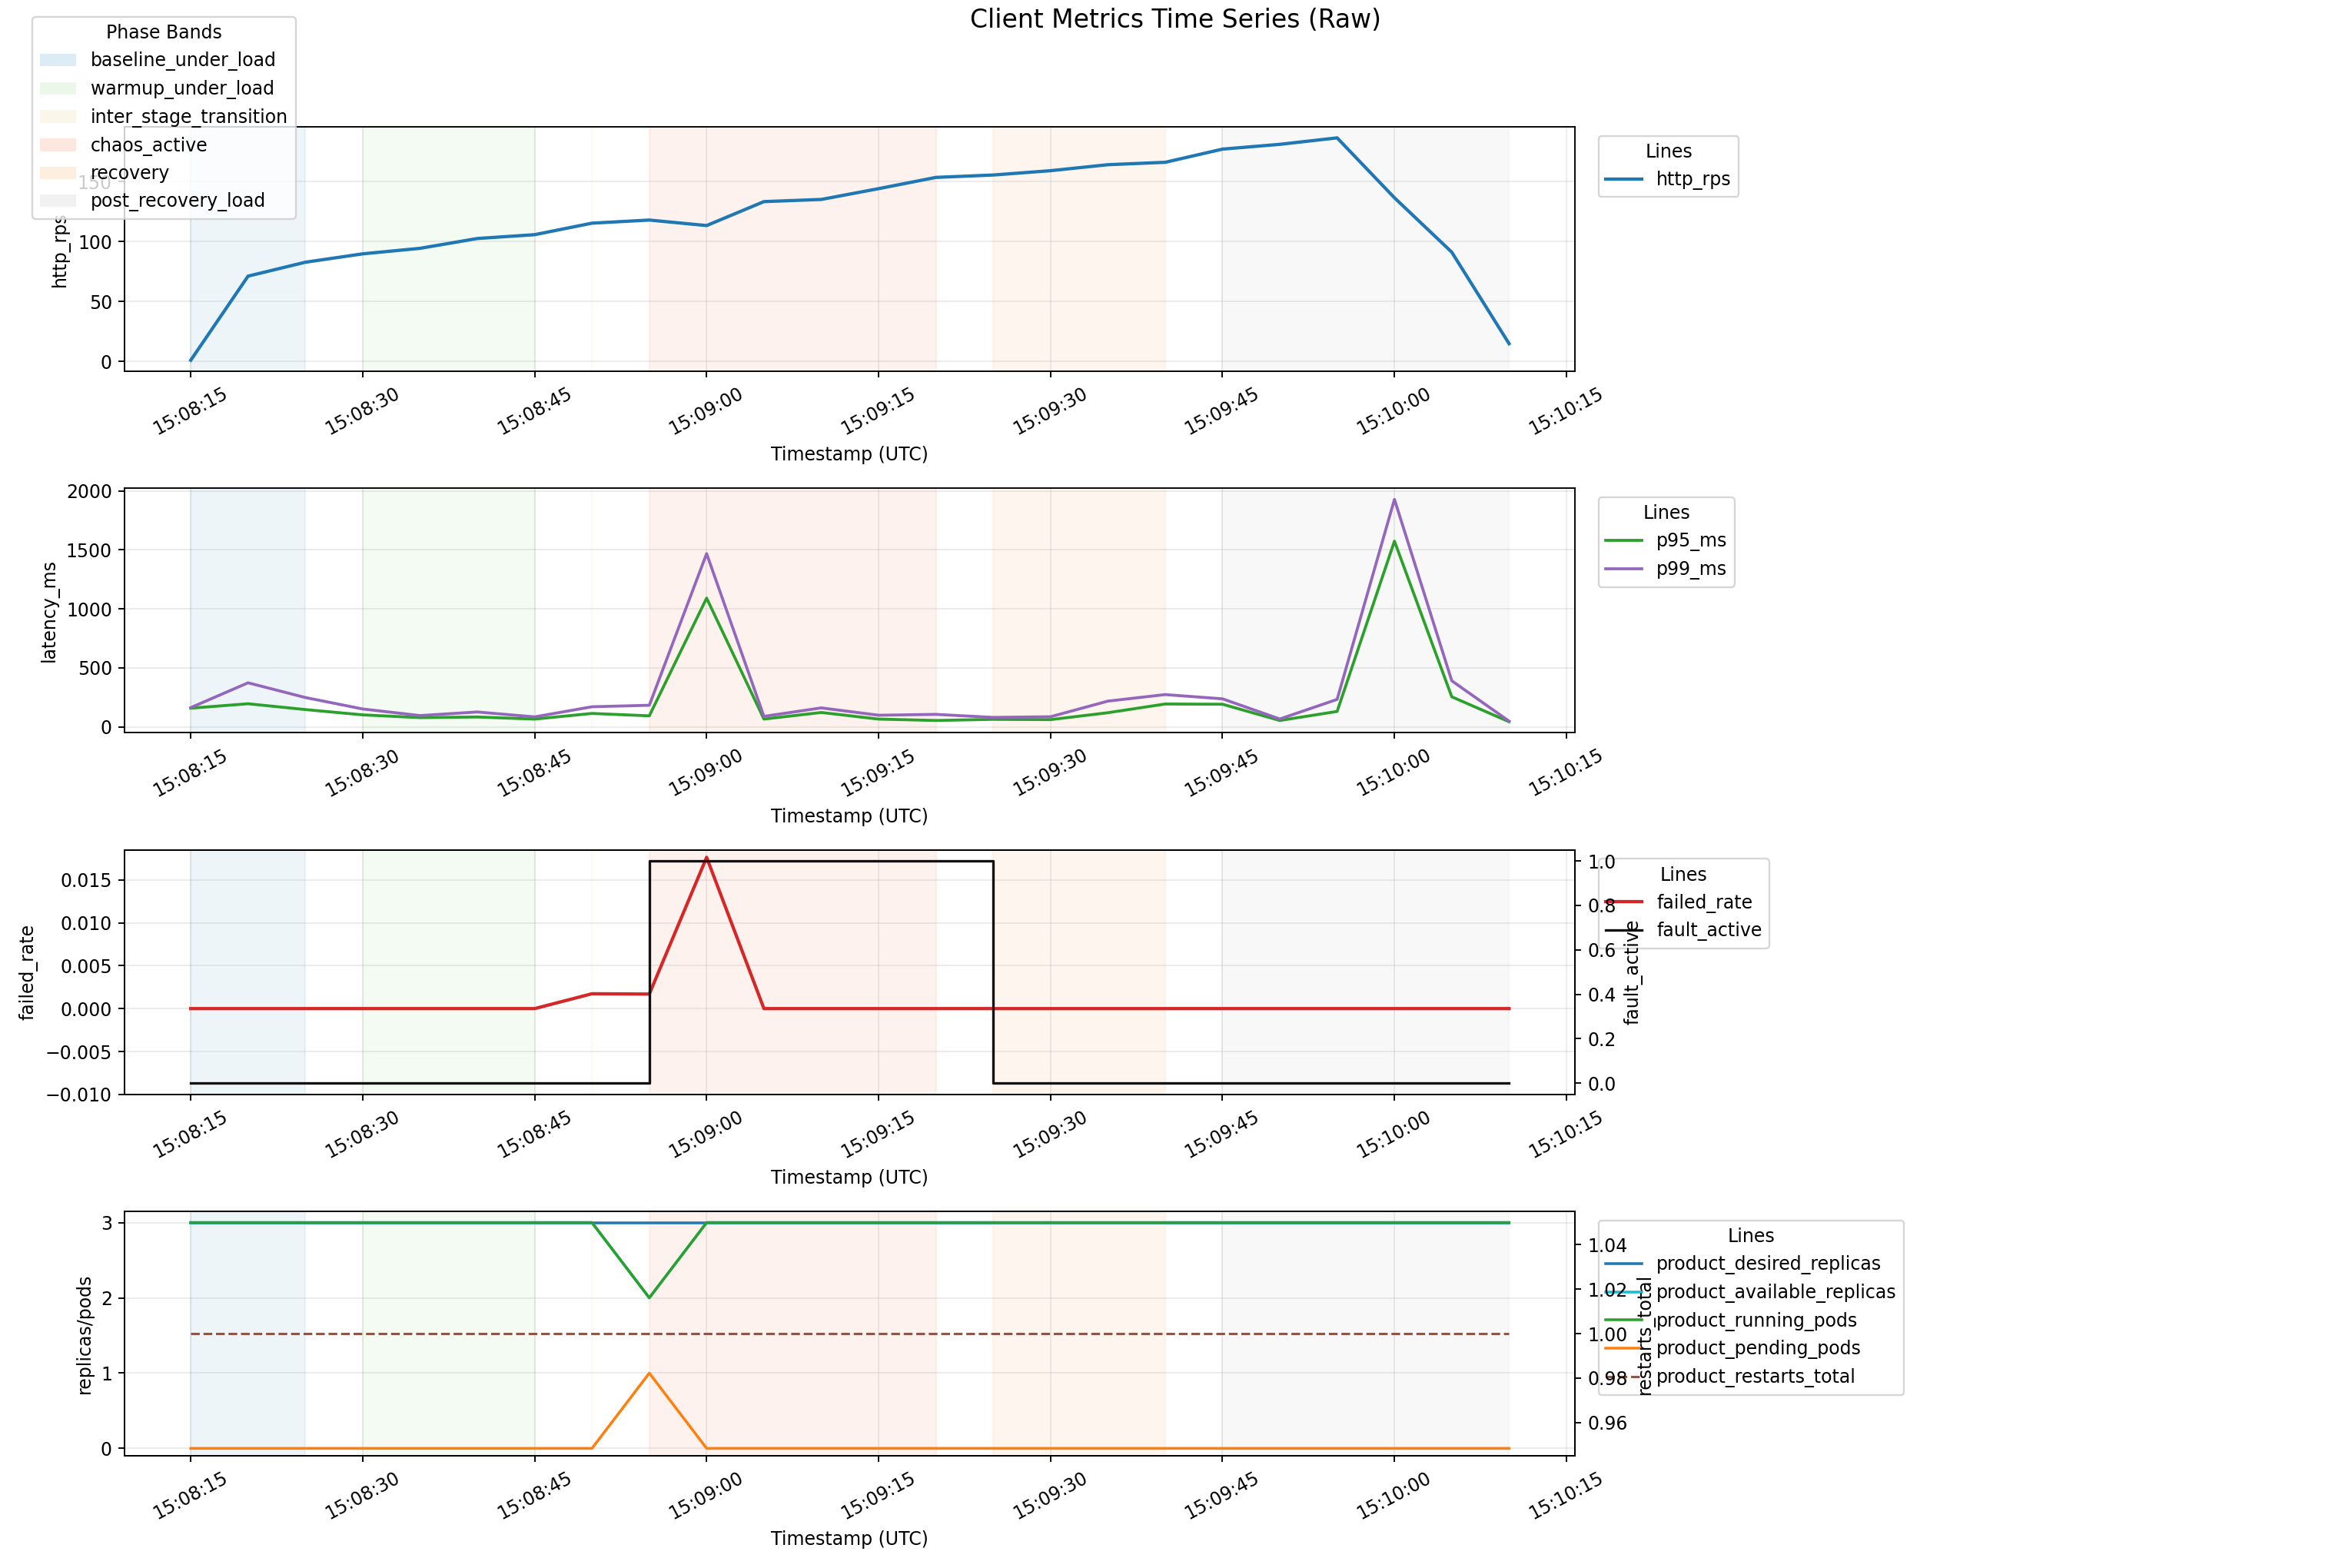
\includegraphics[height=0.5\textheight,keepaspectratio]{graphics/chapter-5/benchmark-norl.png}
    \captionof{figure}{Chuỗi chỉ số phía client và trạng thái workload trong benchmark chưa áp dụng RL}
    \label{fig:benchmark-no-rl-timeseries}
\end{center}

\noindent Từ Hình \ref{fig:benchmark-no-rl-timeseries} có thể quan sát:
\begin{itemize}
    \item Trong pha \textit{chaos-active}, độ trễ p95/p99 xuất hiện các đỉnh tăng mạnh.
    \item \texttt{failed\_rate} tăng ngắn hạn đồng thời với tín hiệu \texttt{fault\_active}.
    \item Số lượng pod \textit{running} có dao động tại thời điểm sự cố trước khi quay về trạng thái ổn định.
\end{itemize}
\noindent Đây là đường cơ sở quan trọng để so sánh mức cải thiện khi áp dụng chính sách tự phục hồi dựa trên RL ở các chương sau.

\begin{center}
    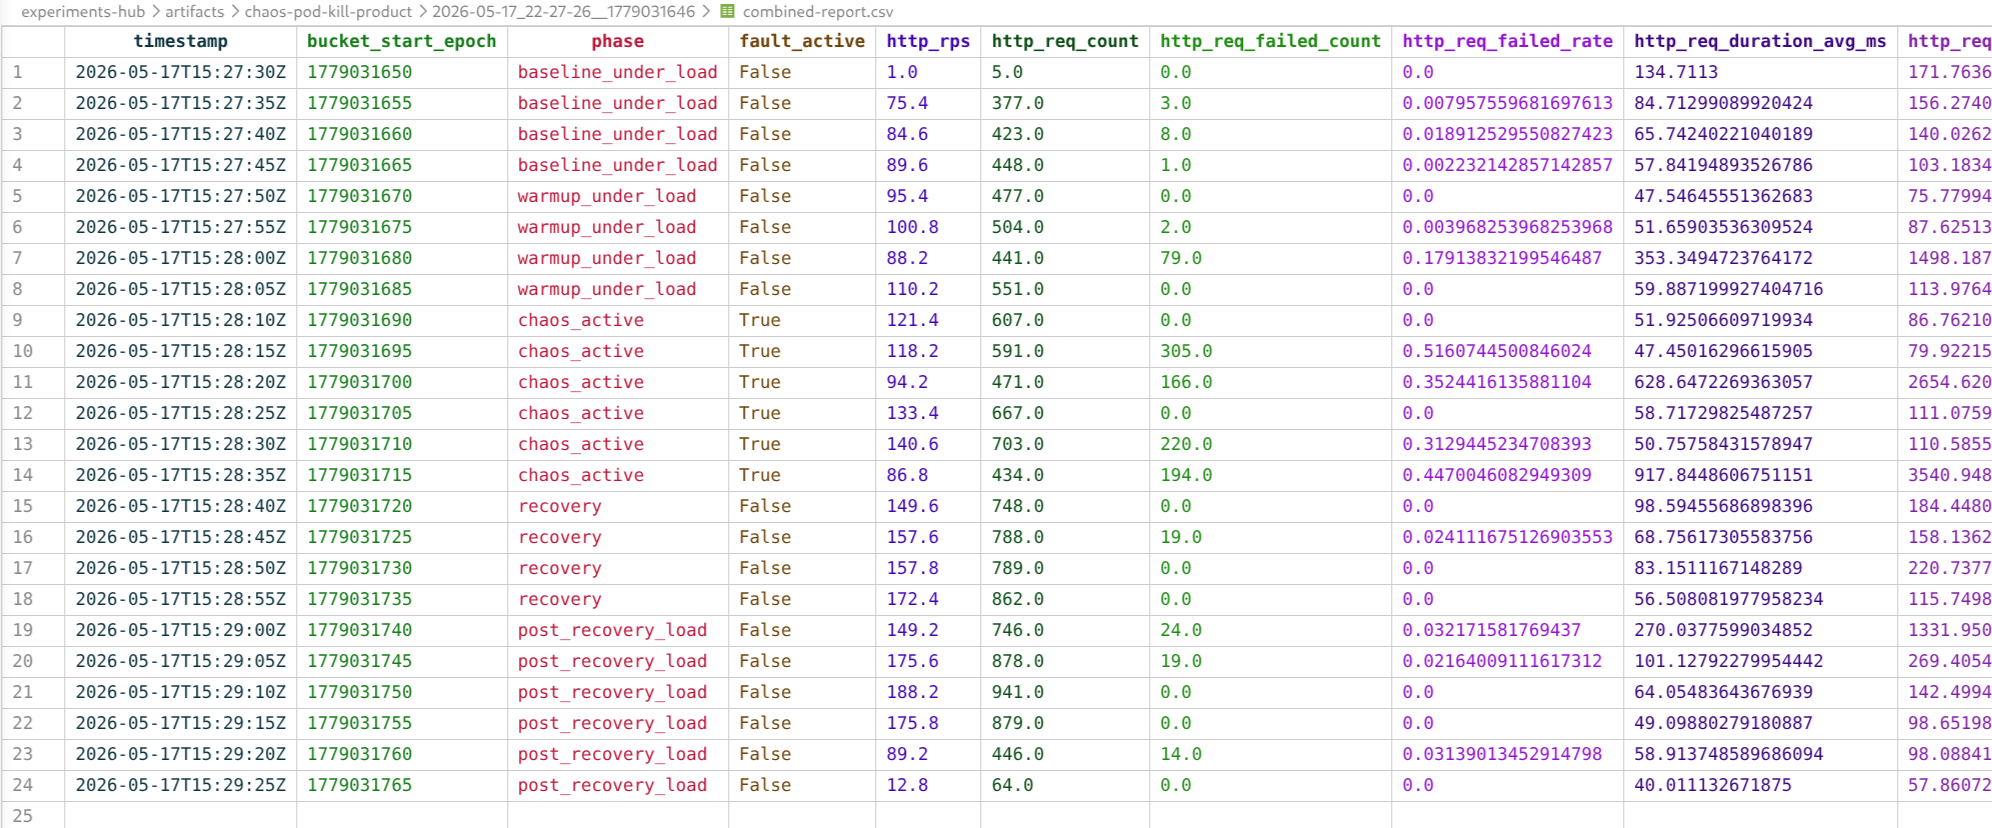
\includegraphics[width=1.0\textwidth]{graphics/chapter-5/metrics.png}
    \captionof{figure}{Trích xuất dữ liệu \texttt{combined-report.csv} sau một lượt chạy benchmark}
    \label{fig:combined-report-csv-snapshot}
\end{center}

\noindent Hình \ref{fig:combined-report-csv-snapshot} cho thấy cấu trúc dữ liệu đầu ra đã được đồng bộ theo bucket 5 giây. Các nhóm trường chính gồm:
\begin{itemize}
    \item Trường thời gian: \texttt{timestamp}, \texttt{bucket\_start\_epoch}.
    \item Trường pha thí nghiệm: \texttt{phase}, \texttt{fault\_active}.
    \item Nhóm chỉ số tải và lỗi:
    \begin{itemize}
        \item \texttt{http\_rps}, \texttt{http\_req\_count}, \texttt{http\_req\_failed\_rate}.
    \end{itemize}
    \item Nhóm chỉ số độ trễ: \texttt{http\_req\_duration\_avg\_ms}, p95, p99.
\end{itemize}
\noindent Cấu trúc này giúp theo dõi biến động hệ thống theo từng pha \textit{baseline}, \textit{chaos-active}, \textit{recovery} và là đầu vào trực tiếp cho bước huấn luyện RL.

\section{Thiết lập huấn luyện RL}

Dữ liệu huấn luyện được lấy từ các tệp \texttt{combined-report.csv} sinh ra sau mỗi lượt chạy benchmark có tải và có tiêm lỗi. Mỗi mẫu dữ liệu đã được đồng bộ theo bucket 5 giây, giữ đầy đủ ngữ cảnh pha thí nghiệm (\textit{baseline}, \textit{warm-up}, \textit{chaos-active}, \textit{recovery}) cùng các chỉ số tải, lỗi và độ trễ.

Trong phạm vi đồ án, quá trình huấn luyện tập trung vào kịch bản \textbf{Pod Failure}, sử dụng dữ liệu từ thí nghiệm \texttt{chaos-pod-kill-product}.

\subsection{Huấn luyện tác nhân DQN}

Đối với DQN, dữ liệu artifact được nạp thành nhiều quỹ đạo trạng thái. Sau đó, môi trường \texttt{ArtifactReplayEnv} được khởi tạo để mô phỏng lại diễn biến của hệ thống theo từng episode, đồng thời cho phép hành động của tác nhân tác động lên trạng thái kế tiếp. Tác nhân DQN sử dụng chính sách \textit{epsilon-greedy}, kết hợp \textit{replay buffer} và \textit{target network} để ổn định quá trình cập nhật giá trị Q.

Các siêu tham số huấn luyện được cấu hình tập trung và được hiệu chỉnh lại theo từng lượt chạy thực nghiệm. Trong cấu hình DQN dùng cho kịch bản \textit{Pod Failure}, các tham số chính được trình bày trong Bảng \ref{tab:dqn-hyperparameters}.

\begin{center}
\captionof{table}{Một số siêu tham số chính trong cấu hình huấn luyện DQN}
\label{tab:dqn-hyperparameters}
\footnotesize
\renewcommand{\arraystretch}{1.0}
\begin{tabular}{|L{4.9cm}|C{2.3cm}|L{7.6cm}|}
\hline
\textbf{Tham số} & \textbf{Giá trị} & \textbf{Vai trò} \\ \hline
\texttt{timesteps} & \texttt{400000} & Tổng số bước huấn luyện của tác nhân DQN trên môi trường replay. \\ \hline
\texttt{eval\_episodes} & \texttt{40} & Số episode dùng để đánh giá định kỳ sau huấn luyện. \\ \hline
\texttt{max\_steps} & \texttt{80} & Giới hạn số bước tối đa trong mỗi episode. \\ \hline
\texttt{learning\_rate} & \texttt{5e-5} & Tốc độ cập nhật trọng số của mạng Q chính. \\ \hline
\texttt{buffer\_size} & \texttt{200000} & Kích thước bộ nhớ kinh nghiệm dùng để lưu các mẫu chuyển trạng thái. \\ \hline
\texttt{learning\_starts} & \texttt{10000} & Số bước tích lũy ban đầu trước khi bắt đầu cập nhật mạng Q. \\ \hline
\texttt{batch\_size} & \texttt{256} & Số mẫu được lấy trong mỗi lần cập nhật mini-batch. \\ \hline
\texttt{gamma} & \texttt{0.995} & Hệ số chiết khấu, ưu tiên phần thưởng dài hạn trong quá trình học. \\ \hline
\makecell[l]{\texttt{train\_freq}\\\texttt{gradient\_steps}} & \texttt{4 / 2} & Chu kỳ lấy mẫu cập nhật và số bước tối ưu hóa được thực hiện sau mỗi lần học. \\ \hline
\makecell[l]{\texttt{target\_update\_}\\\texttt{interval}} & \texttt{2000} & Chu kỳ đồng bộ từ mạng Q chính sang mạng mục tiêu để giảm dao động. \\ \hline
\makecell[l]{\texttt{exploration\_initial\_eps}\\to \texttt{exploration\_final\_eps}} & \texttt{1.0 -> 0.05} & Lịch giảm epsilon trong chiến lược \textit{epsilon-greedy}, chuyển dần từ khám phá sang khai thác. \\ \hline
\makecell[l]{\texttt{exploration\_}\\\texttt{fraction}} & \texttt{0.25} & Tỷ lệ tiến trình huấn luyện dành cho giai đoạn giảm epsilon. \\ \hline
\texttt{rolling\_window} & \texttt{40} & Cửa sổ làm mượt dùng khi theo dõi đường hội tụ trong quá trình huấn luyện. \\ \hline
\texttt{dynamics\_mode} & \makecell[c]{\texttt{hybrid\_}\\\texttt{controlled}} & Chế độ mô phỏng động học môi trường khi replay từ dữ liệu artifact. \\ \hline
\texttt{noise\_scale} & \texttt{0.7} & Mức nhiễu bổ sung nhằm tránh tác nhân học quá khớp với một quỹ đạo cố định. \\ \hline
\texttt{seed} & \texttt{42} & Hạt giống ngẫu nhiên để tái lập thí nghiệm. \\ \hline
\end{tabular}
\end{center}

Trong quá trình huấn luyện, mô hình được theo dõi thông qua các chỉ số như phần thưởng theo episode, epsilon, loss và hiệu quả đánh giá sau huấn luyện. Kết quả mỗi lượt chạy được lưu dưới dạng mô hình DQN, các biểu đồ hội tụ và tệp metadata, làm cơ sở cho bước so sánh ở Chương 6.

\subsection{Huấn luyện tác nhân A2C}

Đối với A2C, dữ liệu artifact cũng được nạp thành nhiều quỹ đạo trạng thái và replay trên môi trường \texttt{ArtifactReplayEnv} để tái hiện diễn biến của hệ thống theo từng episode. Khác với DQN, A2C tối ưu đồng thời mạng chính sách (actor) và mạng giá trị (critic), nhờ đó tác nhân học trực tiếp phân phối hành động trên tập hành động rời rạc gồm \texttt{idle}, \texttt{restart\_pod}, \texttt{scale\_up} và \texttt{scale\_down}. Cách tiếp cận này phù hợp với bài toán self-healing khi cần giữ cân bằng giữa khả năng khám phá và độ ổn định của cập nhật trên dữ liệu benchmark có nhiễu.

Các siêu tham số huấn luyện được cấu hình tập trung và được hiệu chỉnh lại theo từng lượt chạy thực nghiệm. Trong cấu hình A2C dùng cho kịch bản \textit{Pod Failure}, các tham số chính được trình bày trong Bảng \ref{tab:a2c-hyperparameters}.

\begin{center}
\captionof{table}{Một số siêu tham số chính trong cấu hình huấn luyện A2C}
\label{tab:a2c-hyperparameters}
\footnotesize
\renewcommand{\arraystretch}{1.0}
\begin{tabular}{|L{4.0cm}|C{2.3cm}|L{8.7cm}|}
\hline
\textbf{Tham số} & \textbf{Giá trị} & \textbf{Vai trò} \\ \hline
\texttt{timesteps} & \texttt{300000} & Tổng số bước huấn luyện của tác nhân A2C trên môi trường replay. \\ \hline
\texttt{eval\_episodes} & \texttt{40} & Số episode dùng để đánh giá định kỳ sau huấn luyện. \\ \hline
\texttt{max\_steps} & \texttt{80} & Giới hạn số bước tối đa trong mỗi episode. \\ \hline
\texttt{min\_traj\_len} & \texttt{20} & Độ dài quỹ đạo tối thiểu để một đoạn dữ liệu được dùng cho huấn luyện. \\ \hline
\texttt{learning\_rate} & \texttt{1e-4} & Tốc độ cập nhật tham số cho actor và critic. \\ \hline
\texttt{n\_steps} & \texttt{64} & Số bước rollout được thu thập trước mỗi lần cập nhật A2C. \\ \hline
\texttt{gamma} & \texttt{0.995} & Hệ số chiết khấu, nhấn mạnh lợi ích dài hạn của chuỗi phục hồi. \\ \hline
\texttt{gae\_lambda} & \texttt{0.97} & Tham số làm trơn ước lượng advantage để giảm phương sai. \\ \hline
\texttt{ent\_coef} & \texttt{0.001} & Hệ số entropy giúp duy trì mức khám phá phù hợp trong giai đoạn đầu. \\ \hline
\texttt{vf\_coef} & \texttt{0.5} & Trọng số của hàm mất mát giá trị trong tối ưu tổng thể. \\ \hline
\texttt{rolling\_window} & \texttt{40} & Cửa sổ làm mượt dùng khi theo dõi đường hội tụ trong quá trình huấn luyện. \\ \hline
\texttt{dynamics\_mode} & \makecell[c]{\texttt{hybrid\_}\\\texttt{controlled}} & Chế độ mô phỏng động học môi trường khi replay từ dữ liệu artifact. \\ \hline
\texttt{noise\_scale} & \texttt{0.65} & Mức nhiễu bổ sung giúp tác nhân tránh học quá khớp theo một quỹ đạo cố định. \\ \hline
\texttt{seed} & \texttt{42} & Hạt giống ngẫu nhiên để tái lập thí nghiệm. \\ \hline
\end{tabular}
\end{center}

Trong quá trình huấn luyện, mô hình A2C được theo dõi thông qua phần thưởng theo episode, độ dài episode, entropy và hiệu quả đánh giá sau huấn luyện. Kết quả mỗi lượt chạy được lưu dưới dạng mô hình A2C, các biểu đồ hội tụ và tệp metadata, làm cơ sở cho bước so sánh với DQN, PPO và baseline ở Chương 6.

\subsection{Huấn luyện tác nhân PPO}

Với PPO, cùng một tập trajectory và cùng môi trường \texttt{ArtifactReplayEnv} được sử dụng để bảo đảm so sánh công bằng với DQN. Mô hình học trực tiếp chính sách trên không gian trạng thái đã được ánh xạ từ dữ liệu benchmark, nhờ đó phù hợp với bài toán phục hồi theo chuỗi quyết định liên tục qua từng bước thời gian.

Các siêu tham số huấn luyện được cấu hình tập trung và được hiệu chỉnh lại theo từng lượt chạy thực nghiệm. Trong cấu hình PPO dùng cho kịch bản \textit{Pod Failure}, các tham số chính được trình bày trong Bảng \ref{tab:ppo-hyperparameters}.

\begin{center}
\captionof{table}{Một số siêu tham số chính trong cấu hình huấn luyện PPO}
\label{tab:ppo-hyperparameters}
\footnotesize
\renewcommand{\arraystretch}{1.0}
\begin{tabular}{|L{4.3cm}|C{2.3cm}|L{7.9cm}|}
\hline
\textbf{Tham số} & \textbf{Giá trị} & \textbf{Vai trò} \\ \hline
\texttt{timesteps} & \texttt{400000} & Tổng số bước huấn luyện của tác nhân PPO trên môi trường replay. \\ \hline
\texttt{eval\_episodes} & \texttt{40} & Số episode dùng để đánh giá định kỳ sau huấn luyện. \\ \hline
\texttt{max\_steps} & \texttt{80} & Giới hạn số bước tối đa trong mỗi episode huấn luyện. \\ \hline
\texttt{min\_traj\_len} & \texttt{20} & Độ dài quỹ đạo tối thiểu để một đoạn dữ liệu được dùng cho huấn luyện. \\ \hline
\texttt{learning\_rate} & \texttt{1e-4} & Tốc độ cập nhật tham số của mạng chính sách và mạng giá trị. \\ \hline
\texttt{n\_steps} & \texttt{2048} & Số bước rollout được thu thập trước mỗi lần cập nhật PPO. \\ \hline
\texttt{batch\_size} & \texttt{128} & Kích thước mini-batch dùng khi tối ưu trên dữ liệu rollout. \\ \hline
\texttt{gamma} & \texttt{0.995} & Hệ số chiết khấu cho phần thưởng dài hạn trong quá trình học. \\ \hline
\texttt{gae\_lambda} & \texttt{0.97} & Hệ số GAE giúp ước lượng advantage ổn định hơn. \\ \hline
\texttt{rolling\_window} & \texttt{40} & Cửa sổ làm mượt dùng khi theo dõi đường hội tụ trong quá trình huấn luyện. \\ \hline
\texttt{dynamics\_mode} & \makecell[c]{\texttt{hybrid\_}\\\texttt{controlled}} & Chế độ mô phỏng động học môi trường khi replay từ dữ liệu artifact. \\ \hline
\texttt{noise\_scale} & \texttt{0.65} & Mức nhiễu bổ sung nhằm tránh tác nhân học quá khớp theo một quỹ đạo cố định. \\ \hline
\texttt{seed} & \texttt{42} & Hạt giống ngẫu nhiên để tái lập thí nghiệm. \\ \hline
\end{tabular}
\end{center}

Sau khi hoàn tất huấn luyện, tác nhân PPO được đánh giá trên nhiều episode và đối chiếu với tác nhân baseline ngẫu nhiên. Kết quả mỗi lượt chạy được lưu dưới dạng mô hình PPO, các biểu đồ hội tụ và tệp metadata, từ đó hỗ trợ phân tích khả năng phục hồi và mức độ ổn định của chính sách học được.

\section{Triển khai mô hình RL trên Kubernetes}

Sau giai đoạn huấn luyện, mô hình RL được đóng gói và đưa trở lại môi trường vận hành dưới dạng các dịch vụ chạy thường trực trên cụm Kubernetes \texttt{k0s}. Cụm này được triển khai trong các private subnet của AWS VPC, nhờ đó toàn bộ thành phần suy luận và thực thi self-healing được đặt gần workload mục tiêu nhưng vẫn giữ nguyên nguyên tắc cô lập mạng và kiểm soát truy cập. Ứng dụng đích trong phạm vi đồ án là hệ thống \texttt{mini-ecommerce}, bao gồm các service \texttt{api-gateway}, \texttt{user-service}, \texttt{inventory-service}, \texttt{order-service}, \texttt{product-service} và \texttt{payment-service}.

Về mặt logic, lớp suy luận RL được bố trí trong namespace riêng \texttt{rl-agent}, tách biệt khỏi namespace ứng dụng nghiệp vụ nhưng vẫn có khả năng quan sát và can thiệp có kiểm soát lên workload mục tiêu thông qua Kubernetes API. Mô hình triển khai này giúp quá trình giám sát, suy luận và thực thi hành động phục hồi diễn ra liên tục trong cùng môi trường thí nghiệm, đồng thời thuận tiện cho việc mở rộng, thay thế phiên bản mô hình hoặc giới hạn phạm vi tác động của tác nhân RL.

\subsection{Kiến trúc triển khai RL Agent}

Kiến trúc triển khai của lớp self-healing dựa trên RL được tổ chức thành ba tầng chức năng: thu thập trạng thái, suy luận chính sách và thực thi hành động. Ở tầng đầu vào, Pod \texttt{metrics-collector} kết nối tới Prometheus và Kubernetes API để lấy các chỉ số vận hành cốt lõi của hệ thống. Các chỉ số này sau đó được chuẩn hóa thành vector trạng thái dùng cho mô hình RL. Ở tầng suy luận, Deployment \texttt{rl-agent} duy trì đồng thời ba bản sao nhằm tăng tính sẵn sàng và hạn chế điểm lỗi đơn lẻ cho thành phần ra quyết định. Ở tầng thực thi, Pod \texttt{action-executor} nhận hành động từ RL Agent và gửi lệnh can thiệp tới Kubernetes API Server.

\noindent Luồng xử lý tổng quát của hệ thống có thể được biểu diễn như sau:

\begin{center}
    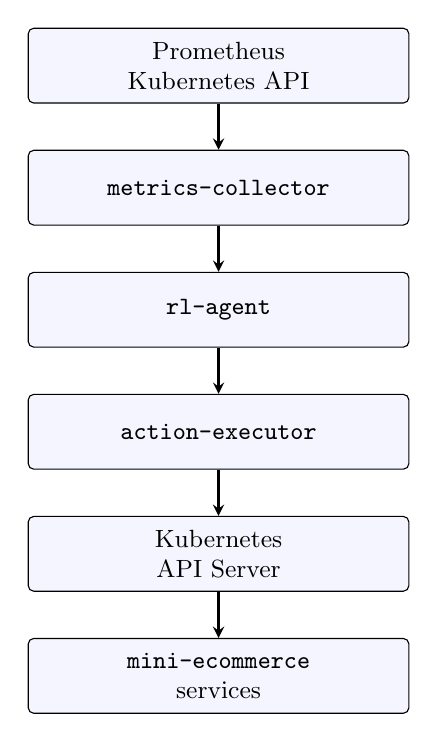
\begin{tikzpicture}[
        >=stealth,
        every node/.style={font=\small},
        flowbox/.style={
            draw,
            rounded corners=2pt,
            align=center,
            minimum height=0.95cm,
            text width=4.6cm,
            fill=blue!4
        }
    ]
        \node[flowbox] (source) at (0,0) {Prometheus\\Kubernetes API};
        \node[flowbox] (collector) at (0,-1.55) {\texttt{metrics-collector}};
        \node[flowbox] (agent) at (0,-3.10) {\texttt{rl-agent}};
        \node[flowbox] (executor) at (0,-4.65) {\texttt{action-executor}};
        \node[flowbox] (apiserver) at (0,-6.20) {Kubernetes\\API Server};
        \node[flowbox] (services) at (0,-7.75) {\texttt{mini-ecommerce}\\services};

        \draw[->, thick] (source) -- (collector);
        \draw[->, thick] (collector) -- (agent);
        \draw[->, thick] (agent) -- (executor);
        \draw[->, thick] (executor) -- (apiserver);
        \draw[->, thick] (apiserver) -- (services);
    \end{tikzpicture}
\end{center}

\noindent Cách bố trí này phù hợp với đặc thù của bài toán self-healing vì nó tách riêng quá trình quan sát trạng thái và thực thi hành động khỏi chính workload mục tiêu. Nhờ đó, ngay cả khi một dịch vụ trong \texttt{mini-ecommerce} gặp lỗi hoặc mất ổn định, lớp điều phối RL vẫn có khả năng tiếp tục hoạt động và đưa ra quyết định phục hồi.

\subsection{Các thành phần chính}

Trong cấu hình hiện tại, lớp RL Agent được triển khai thành tổng cộng năm Pod chính, bao gồm một Pod \texttt{metrics-collector}, ba Pod \texttt{rl-agent} và một Pod \texttt{action-executor}. Vai trò của từng Pod được tóm tắt trong Bảng \ref{tab:rl-agent-pods}.

\begin{center}
\captionof{table}{Các Pod chính trong lớp triển khai RL trên Kubernetes}
\label{tab:rl-agent-pods}
\footnotesize
\renewcommand{\arraystretch}{1.1}
\begin{tabular}{|L{3.2cm}|C{1.8cm}|L{3.1cm}|L{6.5cm}|}
\hline
\textbf{Thành phần} & \textbf{Số Pod} & \textbf{Vai trò chính} & \textbf{Mô tả} \\ \hline
\texttt{metrics-collector} & 1 & Thu thập trạng thái & Lấy metrics từ Prometheus và Kubernetes API, gồm CPU usage, memory usage, request latency p95, error rate, restart count và replica count; sau đó chuyển đổi thành state đầu vào cho mô hình RL. \\ \hline
\texttt{rl-agent} & 3 & Suy luận chính sách & Mỗi Pod nạp mô hình đã huấn luyện, nhận state từ \texttt{metrics-collector} và suy luận một action thuộc tập \texttt{idle}, \texttt{restart pod}, \texttt{scale up}, \texttt{scale down}. Việc duy trì ba replica giúp tăng tính sẵn sàng và khả năng chịu lỗi của thành phần ra quyết định. \\ \hline
\texttt{action-executor} & 1 & Thực thi hành động & Nhận action từ RL Agent, gọi Kubernetes API để \texttt{rollout restart} Deployment, xóa Pod lỗi hoặc thay đổi số replica của Deployment mục tiêu. \\ \hline
\end{tabular}
\end{center}

\noindent Trong ba thành phần trên, \texttt{metrics-collector} đóng vai trò cầu nối giữa lớp observability và mô hình RL. Thành phần này không chỉ lấy dữ liệu thô mà còn thực hiện bước gom nhóm theo cửa sổ thời gian, chuẩn hóa đơn vị đo và ánh xạ các chỉ số sang đúng thứ tự đặc trưng mà mô hình đã sử dụng khi huấn luyện. Điều này giúp giảm sai khác giữa môi trường huấn luyện và môi trường triển khai thực tế.

\noindent Đối với \texttt{rl-agent}, việc triển khai theo dạng Deployment với \texttt{replicas: 3} thay vì chỉ một Pod duy nhất nhằm tránh trường hợp lớp ra quyết định trở thành điểm lỗi đơn. Trong ngữ cảnh self-healing, đây là yêu cầu quan trọng vì khi hệ thống đích đang chịu lỗi, thành phần điều phối phục hồi cần duy trì được khả năng suy luận và phản hồi ổn định.

\noindent Minh họa cấu hình Deployment của \texttt{rl-agent} được trình bày như sau:
\begin{lstlisting}
apiVersion: apps/v1
kind: Deployment
metadata:
  name: rl-agent
  namespace: rl-agent
spec:
  replicas: 3
  selector:
    matchLabels:
      app: rl-agent
  template:
    metadata:
      labels:
        app: rl-agent
    spec:
      serviceAccountName: rl-agent-sa
      containers:
        - name: rl-agent
          image: rl-agent:latest
          env:
            - name: PROMETHEUS_URL
              value: "http://prometheus.monitoring:9090"
            - name: TARGET_NAMESPACE
              value: "mini-ecommerce"
            - name: ACTION_SPACE
              value: "idle,restart,scale_up,scale_down"
          resources:
            requests:
              cpu: "100m"
              memory: "256Mi"
            limits:
              cpu: "500m"
              memory: "1Gi"



\end{lstlisting}

\subsection{Luồng hoạt động self-healing}

Trong quá trình vận hành, các dịch vụ của hệ thống \texttt{mini-ecommerce} liên tục sinh ra dữ liệu quan sát về tài nguyên, độ trễ và tỷ lệ lỗi. Prometheus thu thập các số liệu này theo chu kỳ và lưu trữ dưới dạng time series. Song song với đó, Kubernetes API cung cấp thông tin bổ sung về số replica, trạng thái Pod, số lần restart và các sự kiện vòng đời quan trọng khác.

\noindent Pod \texttt{metrics-collector} định kỳ truy vấn hai nguồn dữ liệu trên để xây dựng trạng thái hiện thời của hệ thống. Trạng thái này phản ánh cả mức tiêu thụ tài nguyên lẫn chất lượng phục vụ của ứng dụng, từ đó tạo đầu vào phù hợp cho bài toán quyết định trong self-healing. Sau khi nhận được state, mỗi Pod \texttt{rl-agent} thực hiện bước suy luận dựa trên policy của mô hình đã được huấn luyện trước đó. Kết quả suy luận là một action trong không gian hành động rời rạc, gồm giữ nguyên trạng thái (\texttt{idle}), khởi động lại Pod lỗi (\texttt{restart pod}), tăng số lượng bản sao (\texttt{scale up}) hoặc giảm số lượng bản sao (\texttt{scale down}).

\noindent Action sau đó được chuyển sang \texttt{action-executor}. Thành phần này đóng vai trò trung gian để tách riêng phần suy luận ra khỏi phần can thiệp hạ tầng. Cách thiết kế này giúp giới hạn bề mặt tấn công của RL Agent, đồng thời cho phép bổ sung thêm các bước kiểm tra an toàn trước khi gửi lệnh xuống Kubernetes API Server. Sau khi hành động được thực thi, trạng thái mới của hệ thống tiếp tục được Prometheus và Kubernetes API ghi nhận, tạo thành vòng lặp quan sát -- quyết định -- can thiệp -- đánh giá liên tục.

\subsection{Cơ chế thực thi action trên Kubernetes}

Từ góc độ triển khai, \texttt{action-executor} là thành phần duy nhất trực tiếp gọi Kubernetes API để thay đổi trạng thái workload. Khi action đầu ra là \texttt{restart pod}, executor có thể chọn một trong hai cách tiếp cận: yêu cầu \texttt{rollout restart} đối với Deployment mục tiêu hoặc xóa trực tiếp Pod đang lỗi để ReplicaSet tạo lại bản sao mới. Khi action là \texttt{scale up} hoặc \texttt{scale down}, executor sẽ cập nhật trường \texttt{spec.replicas} của Deployment tương ứng. Trong trường hợp action là \texttt{idle}, hệ thống chỉ ghi log quyết định và tiếp tục vòng quan sát kế tiếp.

\noindent Để tránh việc tác nhân RL có quyền thao tác quá rộng, cơ chế thực thi được ràng buộc bằng \texttt{ServiceAccount}, \texttt{Role} và \texttt{RoleBinding}. Các quyền này chỉ nên giới hạn trong namespace ứng dụng \texttt{mini-ecommerce} và tập tài nguyên thật sự cần thiết, chủ yếu là \texttt{pods}, \texttt{deployments} và \texttt{deployments/scale}. Cách tiếp cận tối thiểu quyền hạn này giúp giảm rủi ro can thiệp ngoài ý muốn vào các namespace hạ tầng hoặc thành phần quan sát.

\newpage
\noindent Ví dụ rút gọn cho cấu hình quyền thực thi như sau:
\begin{lstlisting}
apiVersion: rbac.authorization.k8s.io/v1
kind: Role
metadata:
  name: rl-agent-role
  namespace: mini-ecommerce
rules:
  - apiGroups: [""]
    resources: ["pods"]
    verbs: ["get", "list", "watch", "delete"]
  - apiGroups: ["apps"]
    resources: ["deployments", "deployments/scale"]
    verbs: ["get", "list", "watch", "patch", "update"]
\end{lstlisting}

\noindent Bên cạnh RBAC, lớp executor cũng có thể áp dụng thêm các guardrail như giới hạn số replica tối thiểu/tối đa, thời gian chờ giữa hai lần can thiệp liên tiếp và cơ chế bỏ qua action nếu trạng thái hệ thống chưa ổn định. Những ràng buộc này không thay thế mô hình RL, nhưng giúp quá trình triển khai thực tế an toàn và nhất quán hơn.

\noindent Tóm lại, mục này tập trung vào cách tổ chức và triển khai lớp RL Agent lên cụm \texttt{k0s} dưới dạng các Pod chuyên biệt cho thu thập trạng thái, suy luận chính sách và thực thi hành động. Cách bố trí này giúp mô hình đã huấn luyện có thể vận hành trực tiếp trong môi trường Kubernetes, đồng thời giữ được tính tách biệt với workload nghiệp vụ và khả năng kiểm soát quyền can thiệp thông qua các cơ chế chuẩn của nền tảng.


\chapter{Kết quả và phân tích}
\label{c:ketquavaphantich}

\section{Kết quả huấn luyện mô hình}

Trong phạm vi thực nghiệm hiện tại, dữ liệu huấn luyện được lấy từ 6 quỹ đạo artifact của kịch bản \texttt{chaos-pod-kill-product}. Các quỹ đạo này đã được ánh xạ về không gian trạng thái MDP và đưa vào môi trường \texttt{ArtifactReplayEnv} để huấn luyện tác nhân. Kết quả được lưu theo từng run, bao gồm mô hình, metadata và các biểu đồ chẩn đoán quá trình học.

\subsection{DQN}

Đối với DQN, mô hình được huấn luyện trong 400\,000 bước thời gian với môi trường động học \texttt{hybrid\_controlled}, hệ số nhiễu \texttt{noise\_scale = 0.70} và 40 episode đánh giá sau huấn luyện. Các siêu tham số chính của run này gồm \textit{learning rate} $= 5\times10^{-5}$, \textit{buffer size} = 200\,000, \textit{batch size} = 256, \textit{target update interval} = 2\,000 và cơ chế thăm dò \textit{epsilon-greedy} giảm từ 1.0 xuống 0.05.

\begin{minipage}{\textwidth}
    \centering
    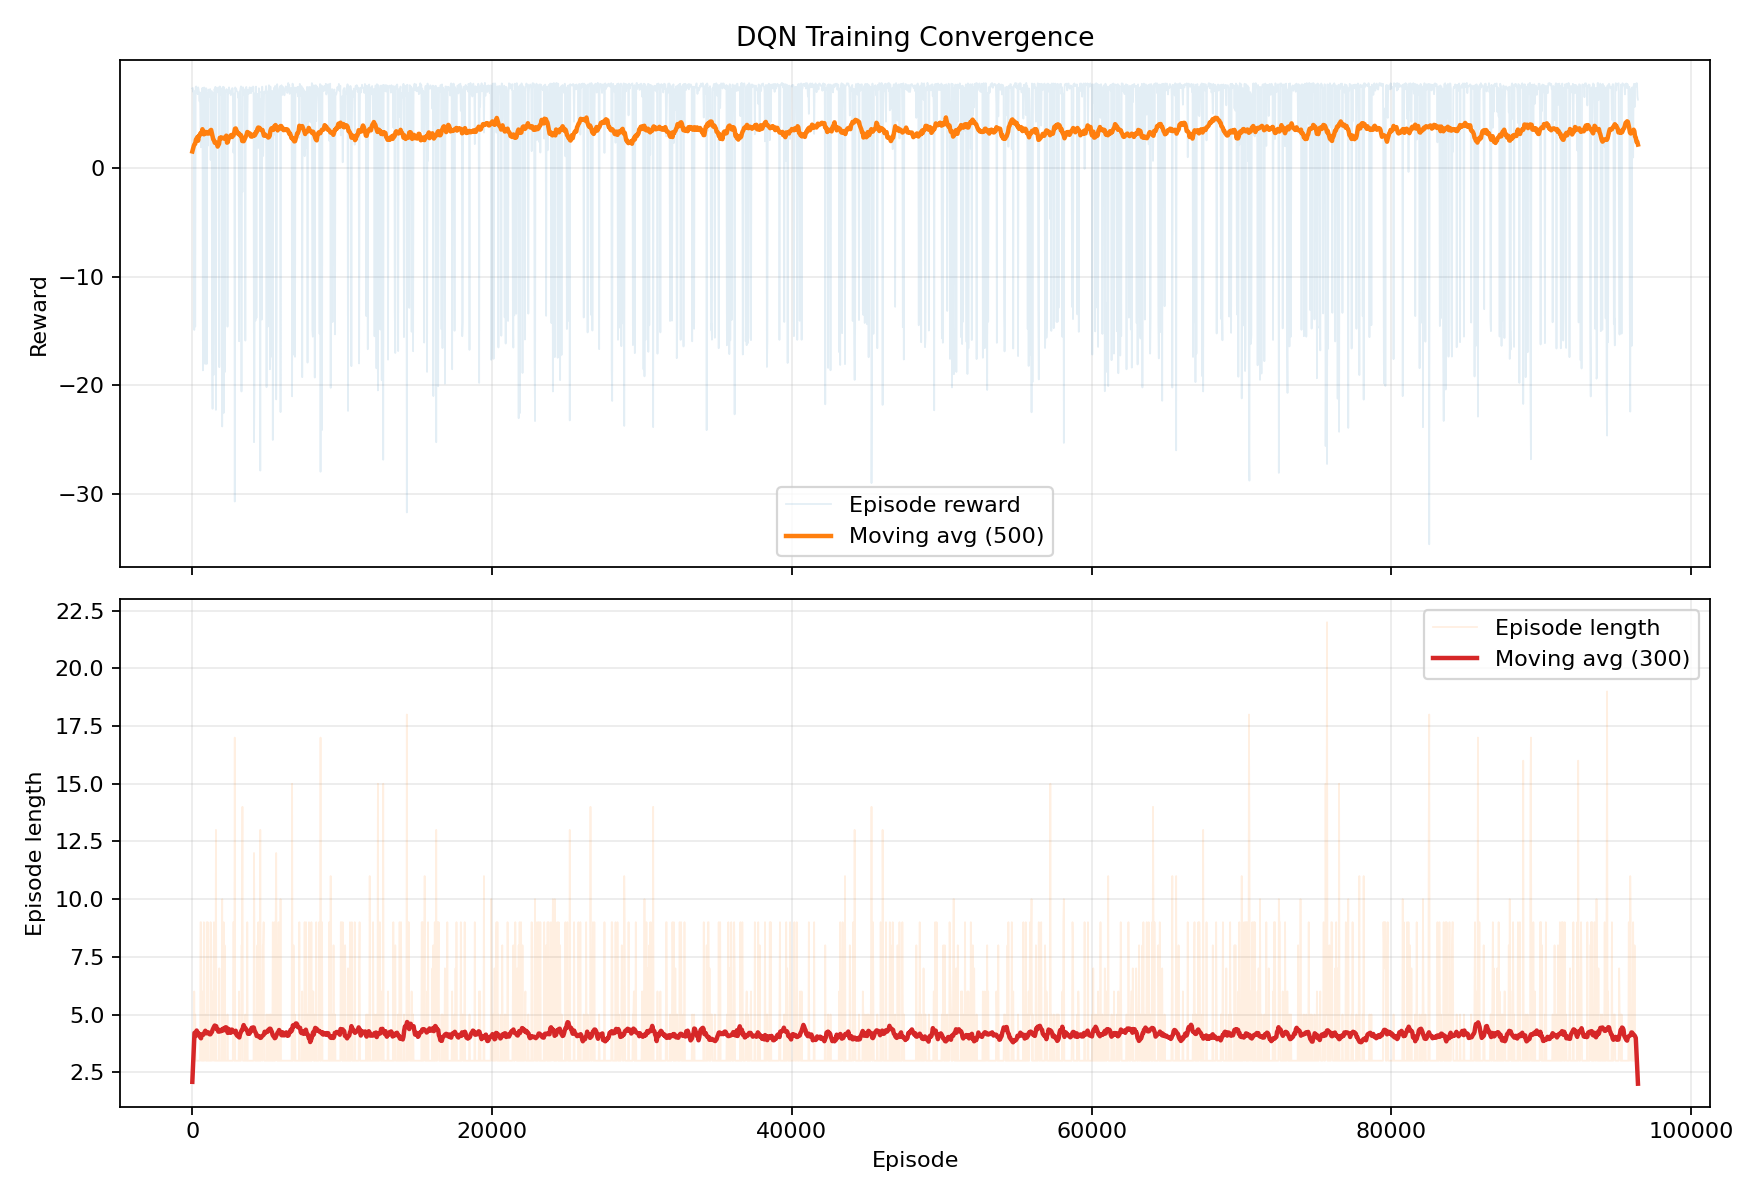
\includegraphics[width=0.95\textwidth]{graphics/chapter-6/train_DQN/training_curve.png}
    \captionsetup{hypcap=false}
    \captionof{figure}{Biểu đồ hội tụ theo phần thưởng và độ dài episode của DQN}
    \label{fig:dqn-training-convergence}
\end{minipage}

\noindent Hình \ref{fig:dqn-training-convergence} biểu diễn sự biến thiên của phần thưởng theo episode và độ dài episode của DQN trong quá trình huấn luyện. Đường màu xanh nhạt và màu cam nhạt biểu thị điểm thưởng tức thời và độ dài episode thực tế, trong khi các đường đậm nét thể hiện giá trị trung bình trượt tương ứng. Có thể thấy điểm thưởng trung bình tăng dần và tiệm cận mức ổn định quanh giá trị 3.0--4.0. Đồng thời, độ dài của episode nhanh chóng hội tụ về khoảng 4 bước hành động, cho thấy tác nhân đã tìm ra cách khôi phục hệ thống hiệu quả và rút ngắn thời gian xử lý sự cố.

\begin{minipage}{\textwidth}
    \centering
    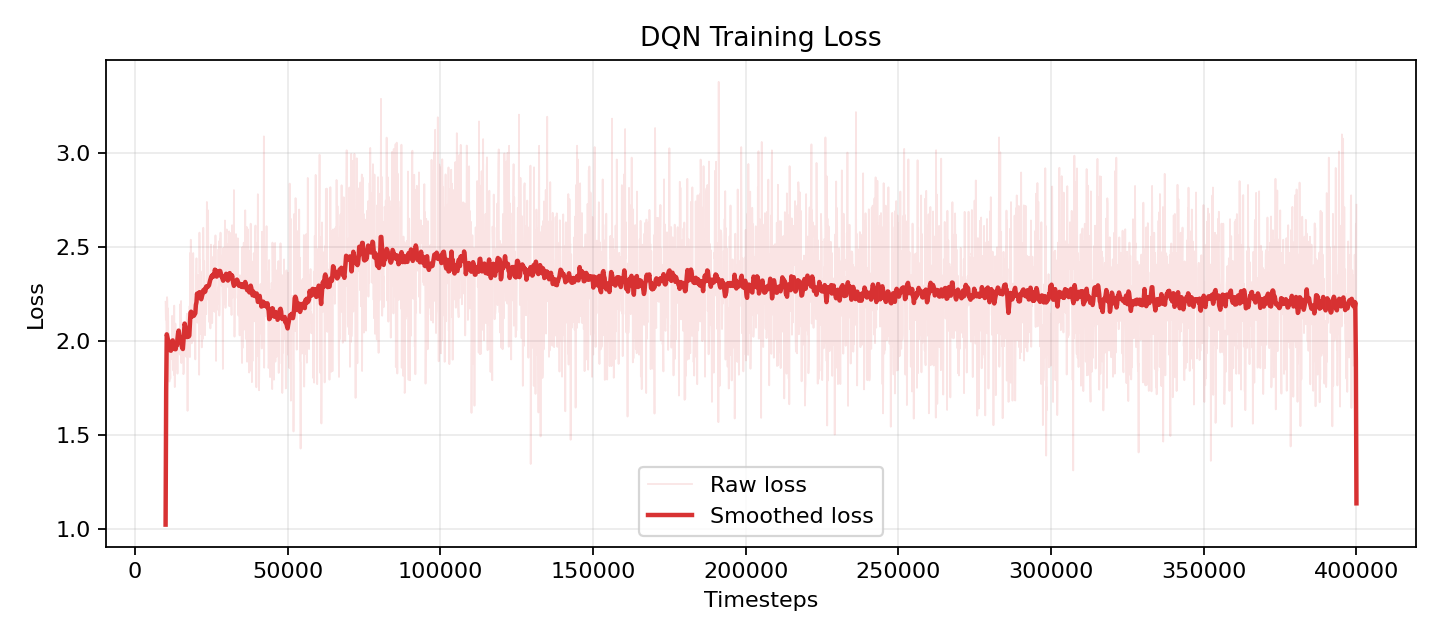
\includegraphics[width=0.9\textwidth]{graphics/chapter-6/train_DQN/loss_curve.png}
    \captionsetup{hypcap=false}
    \captionof{figure}{Biến thiên hàm mất mát (\textit{training loss}) của DQN}
    \label{fig:dqn-loss}
\end{minipage}

\noindent Đường biểu diễn hàm mất mát của mạng neural được trình bày ở Hình \ref{fig:dqn-loss}. Ở giai đoạn đầu, giá trị loss tăng vọt lên khoảng 2.5 do tác nhân bắt đầu khám phá và lưu trữ dữ liệu vào bộ nhớ đệm (\textit{replay buffer}), dẫn đến sai lệch lớn trong các bước cập nhật trọng số. Tuy nhiên, sau khoảng 80\,000 bước thời gian, hàm loss đi ngang và duy trì trạng thái ổn định quanh mức 2.2 cho tới cuối quá trình huấn luyện, đảm bảo mạng Q-learning không bị phân kỳ.

\begin{minipage}{\textwidth}
    \centering
    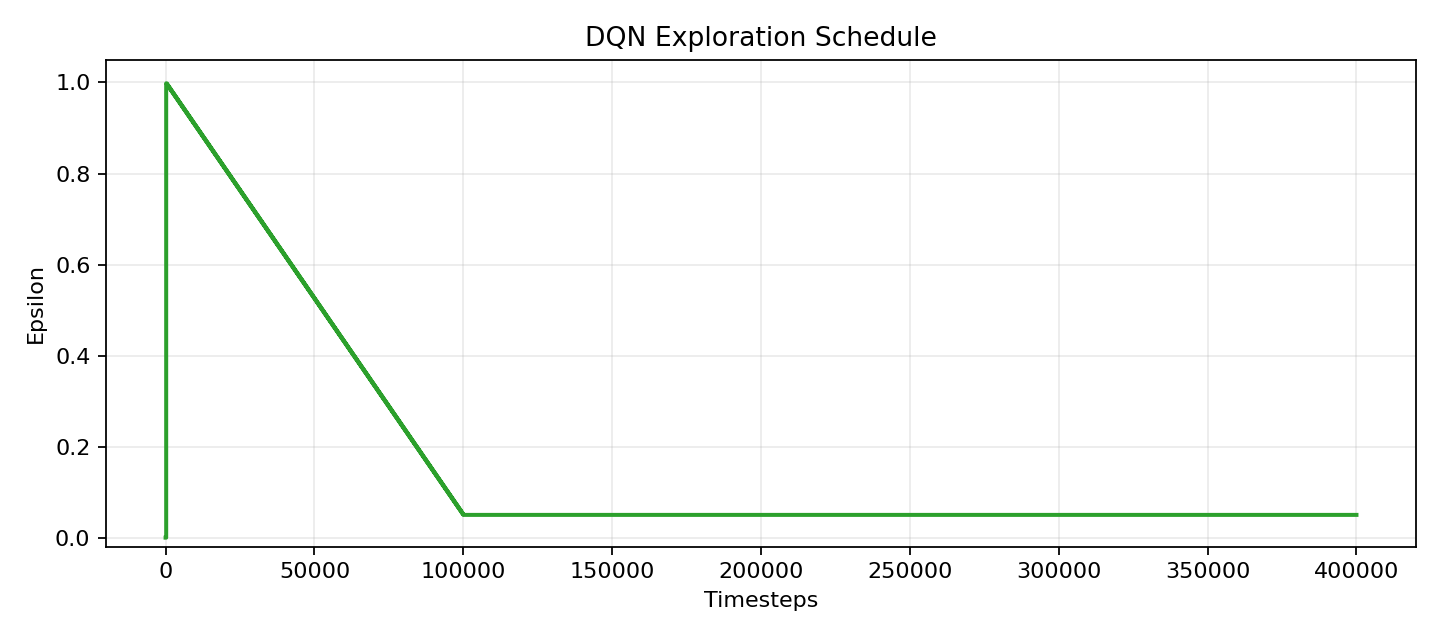
\includegraphics[width=0.9\textwidth]{graphics/chapter-6/train_DQN/epsilon_curve.png}
    \captionsetup{hypcap=false}
    \captionof{figure}{Lịch trình suy giảm hệ số thăm dò \textit{epsilon} của DQN}
    \label{fig:dqn-epsilon}
\end{minipage}

\noindent Lịch trình thăm dò của tác nhân DQN được mô tả ở Hình \ref{fig:dqn-epsilon}. Hệ số $\epsilon$ giảm tuyến tính từ 1.0 xuống 0.05 trong 100\,000 bước huấn luyện đầu tiên (chiếm 25\% tổng thời gian), sau đó giữ cố định ở mức 0.05. Lịch trình này đảm bảo tác nhân có đủ thời gian để khám phá các hành động ngẫu nhiên ở pha đầu trước khi chuyển hẳn sang khai thác chính sách tối ưu ở pha sau.

\begin{minipage}{\textwidth}
    \centering
    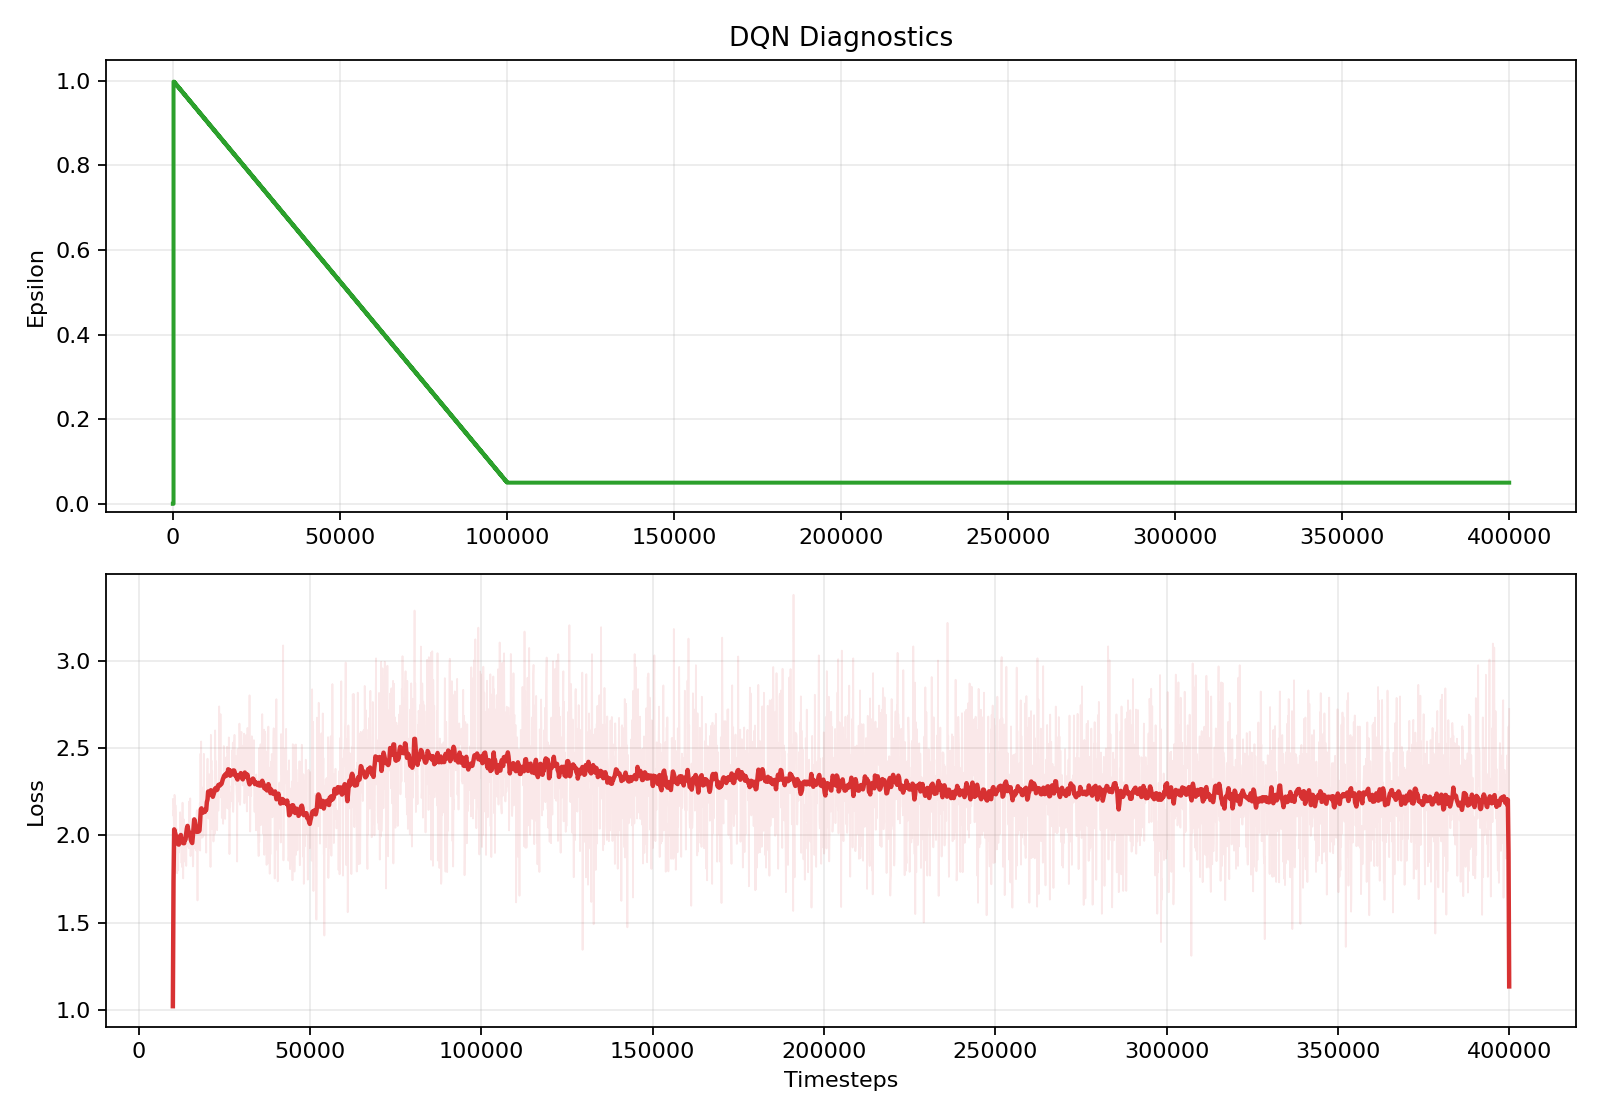
\includegraphics[width=0.92\textwidth]{graphics/chapter-6/train_DQN/dqn_diagnostics.png}
    \captionsetup{hypcap=false}
    \captionof{figure}{Biểu đồ chẩn đoán quá trình huấn luyện DQN tổng hợp}
    \label{fig:dqn-diagnostics-pod-failure}
\end{minipage}

\noindent Hình \ref{fig:dqn-diagnostics-pod-failure} tổng hợp hai chỉ số chẩn đoán quan trọng là hệ số $\epsilon$ và giá trị loss theo các bước thời gian. Sự kết hợp này giúp đối chiếu trực quan tiến trình huấn luyện, xác nhận rằng khi pha khám phá giảm dần, quá trình cập nhật giá trị Q cũng đi vào trạng thái ổn định và hội tụ.

\begin{minipage}{\textwidth}
    \centering
    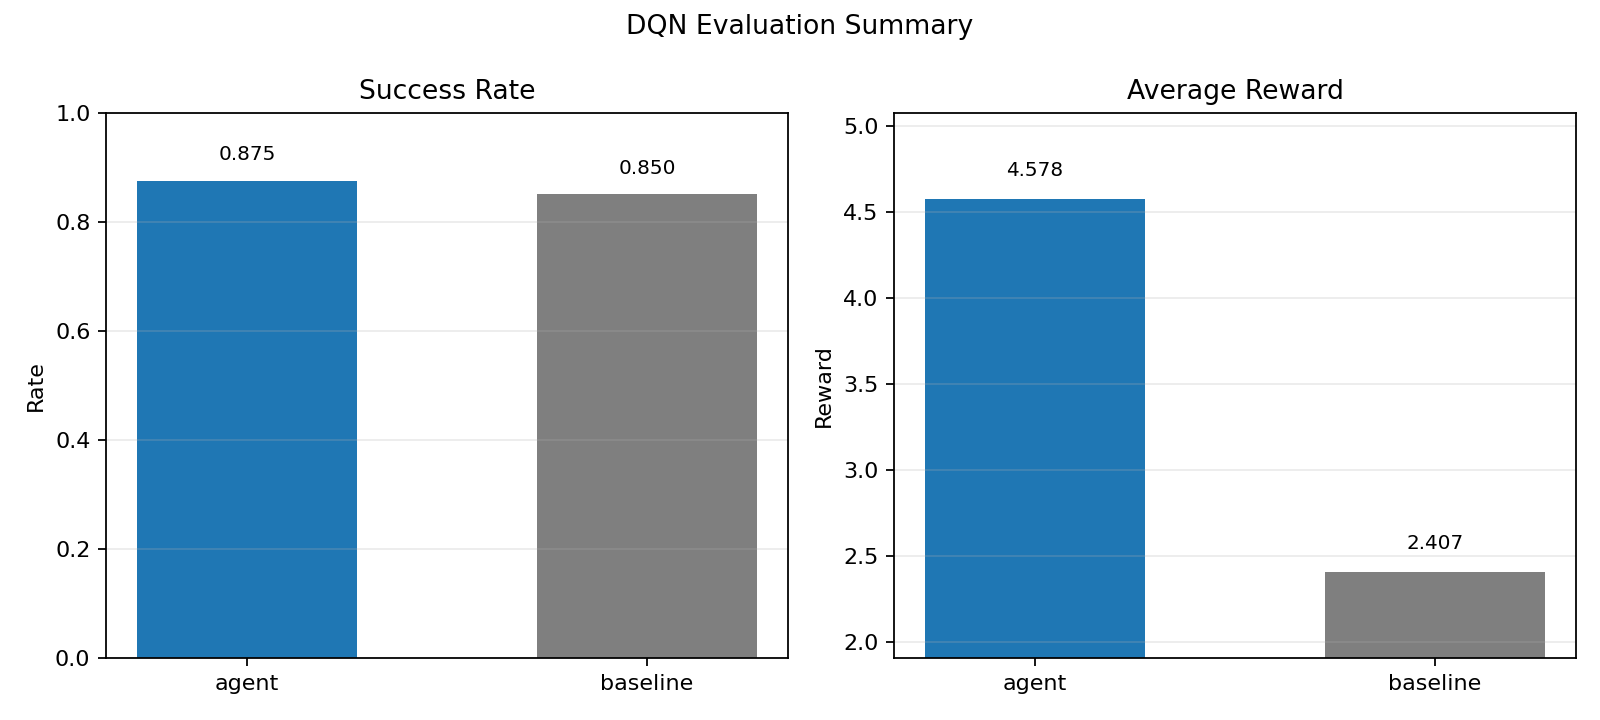
\includegraphics[width=0.92\textwidth]{graphics/chapter-6/train_DQN/evaluation_summary.png}
    \captionsetup{hypcap=false}
    \captionof{figure}{So sánh kết quả đánh giá DQN với baseline}
    \label{fig:dqn-evaluation-summary}
\end{minipage}

\noindent Kết quả đánh giá tác nhân DQN được trình bày ở Hình \ref{fig:dqn-evaluation-summary}. Sau khi hoàn thành huấn luyện, mô hình DQN đạt tỷ lệ phục hồi thành công (\textit{success rate}) là 0.875, cao hơn so với mức 0.850 của baseline ngẫu nhiên. Về mặt tối ưu hóa chi phí và hiệu năng hệ thống, phần thưởng trung bình của DQN đạt 4.578, vượt trội đáng kể so với baseline (2.407). Điều này chứng minh tác nhân đã học được cách giảm thiểu các hành động can thiệp thừa hoặc trùng lặp, nâng cao hiệu quả tự phục hồi cho hệ thống Kubernetes.

\subsection{A2C}

Đối với A2C, mô hình được huấn luyện trong 300\,000 bước thời gian với kịch bản động học \texttt{hybrid\_controlled}, hệ số nhiễu \texttt{noise\_scale = 0.65} và 40 episode đánh giá sau huấn luyện. Các siêu tham số cấu hình chính bao gồm tốc độ học \textit{learning rate} $= 10^{-4}$ (sử dụng lịch trình thay đổi tuyến tính), số bước cập nhật mỗi chu kỳ \textit{n\_steps} = 64, hệ số giảm giá \textit{gamma} = 0.995, tham số \textit{gae\_lambda} = 0.97, hệ số entropy \textit{ent\_coef} = 0.001 và hệ số hàm giá trị \textit{vf\_coef} = 0.5.

\begin{minipage}{\textwidth}
    \centering
    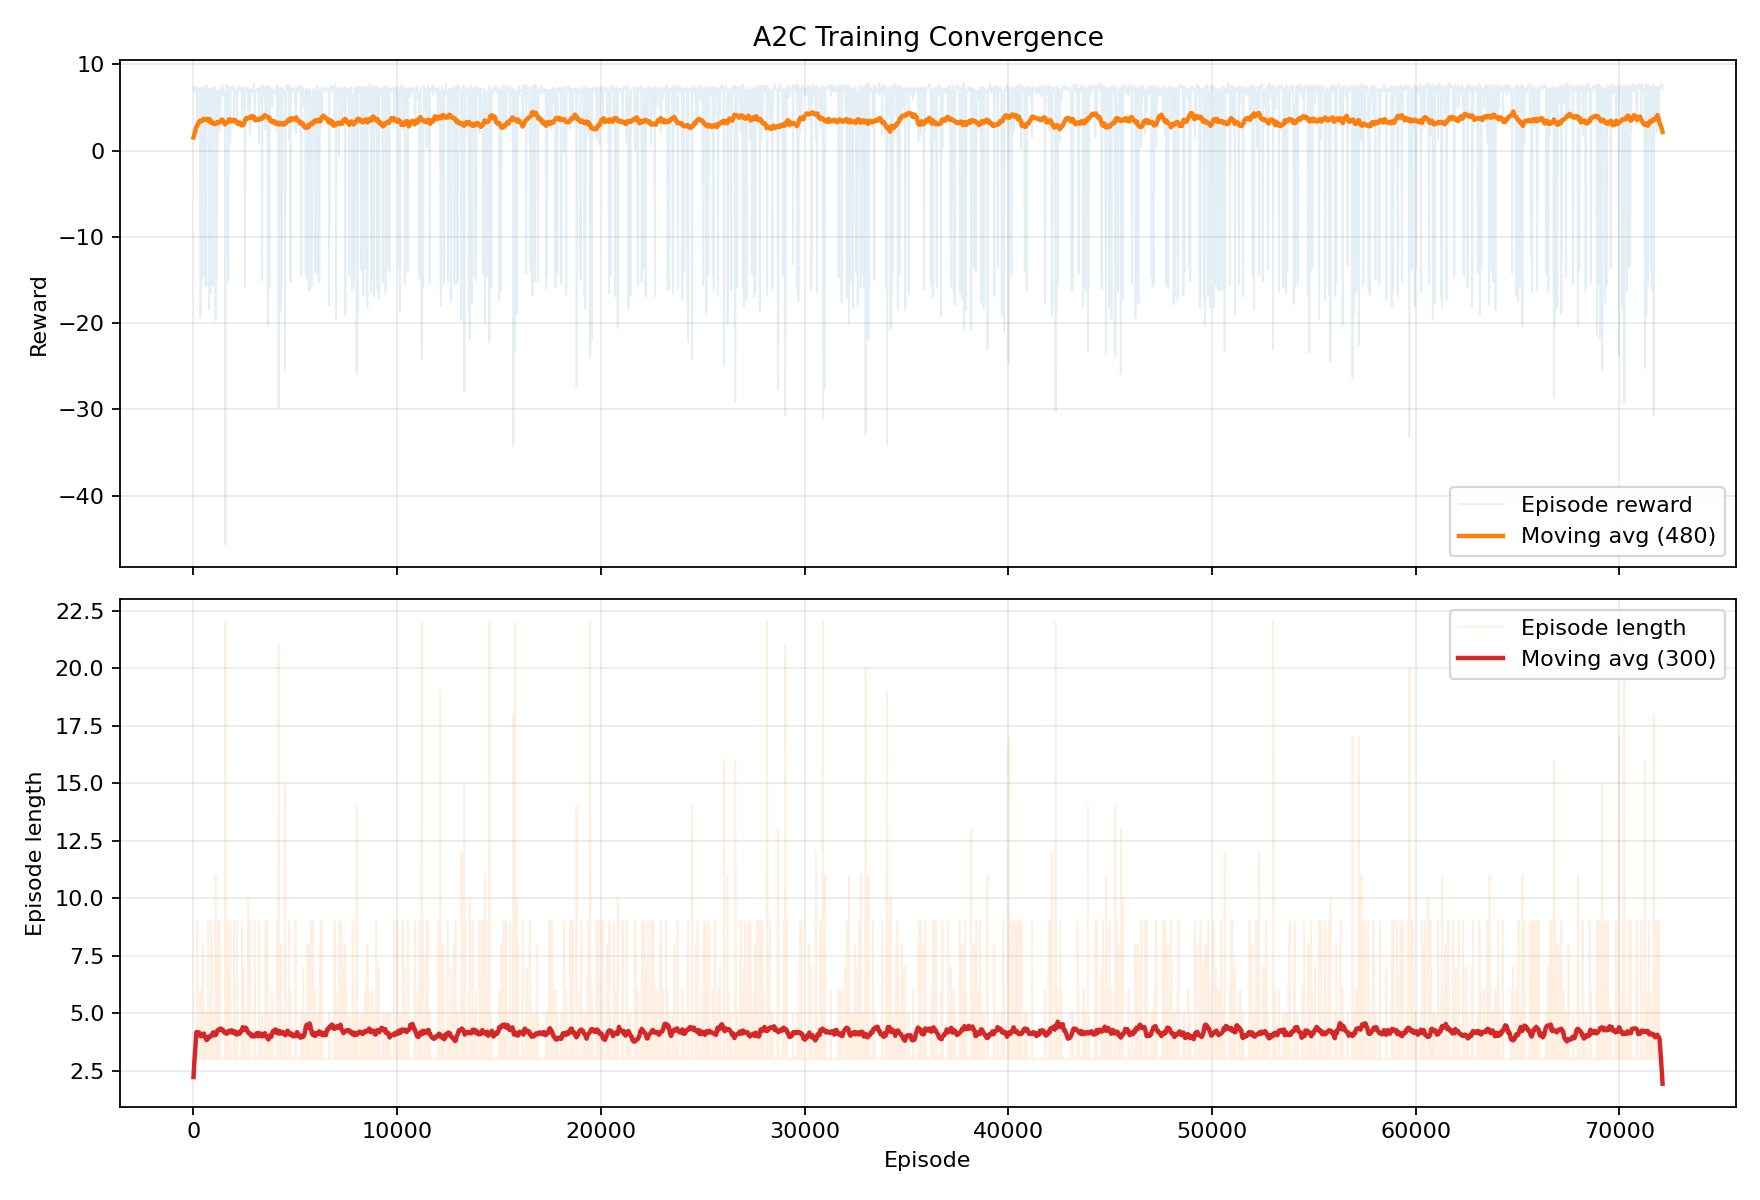
\includegraphics[width=0.95\textwidth]{graphics/chapter-6/train_A2C/training_curve.png}
    \captionsetup{hypcap=false}
    \captionof{figure}{Biểu đồ hội tụ theo phần thưởng và độ dài episode của A2C}
    \label{fig:a2c-training-convergence}
\end{minipage}

\noindent Hình \ref{fig:a2c-training-convergence} mô tả quá trình hội tụ phần thưởng và độ dài episode trong suốt 300\,000 bước huấn luyện của tác nhân A2C. Mặc dù điểm thưởng tức thời (đường màu xanh nhạt) vẫn dao động lớn do tính chất ngẫu nhiên của môi trường K8s giả lập, đường trung bình trượt (đường màu cam) cho thấy xu hướng tăng trưởng rõ nét từ mức 2.0 lên tiệm cận mức 6.5 và ổn định hoàn toàn ở nửa sau quá trình huấn luyện. Đồng thời, độ dài trung bình của mỗi episode (đường màu đỏ) duy trì ổn định quanh mức 4 bước can thiệp, chứng minh tác nhân đã nhanh chóng tìm được phương án phục hồi tối ưu.

\begin{minipage}{\textwidth}
    \centering
    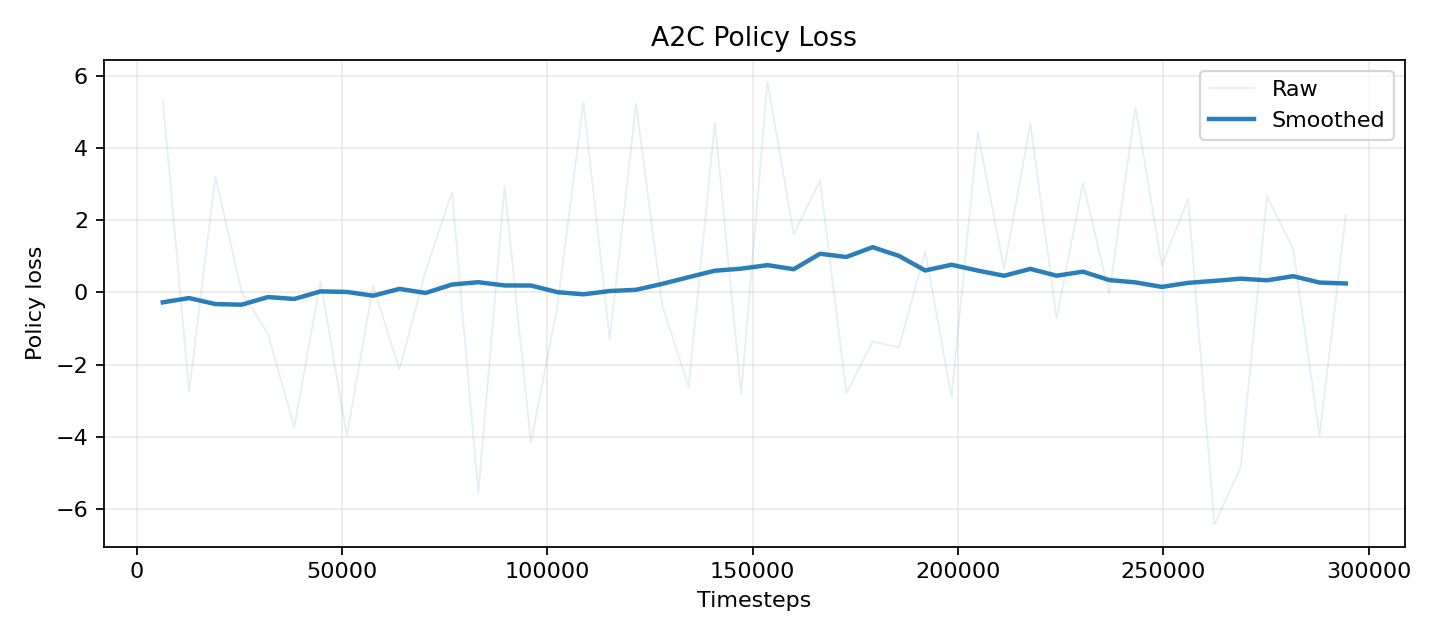
\includegraphics[width=0.9\textwidth]{graphics/chapter-6/train_A2C/policy_loss_curve.png}
    \captionsetup{hypcap=false}
    \captionof{figure}{Biến thiên \textit{policy loss} trong quá trình huấn luyện A2C}
    \label{fig:a2c-policy-loss}
\end{minipage}

\noindent Biến thiên hàm mất mát chính sách (\textit{policy loss}) của A2C được thể hiện trong Hình \ref{fig:a2c-policy-loss}. Do A2C cập nhật chính sách dựa trên hàm lợi thế (\textit{advantage function}), giá trị \textit{policy loss} dao động mạnh quanh điểm cân bằng 0 (trong khoảng [-6, 6]). Tuy nhiên, đường làm mượt (smoothed) cho thấy xu hướng ổn định tiệm cận về sát 0 ở các bước huấn luyện cuối cùng, khẳng định chính sách đã đi vào trạng thái hội tụ cục bộ.

\begin{minipage}{\textwidth}
    \centering
    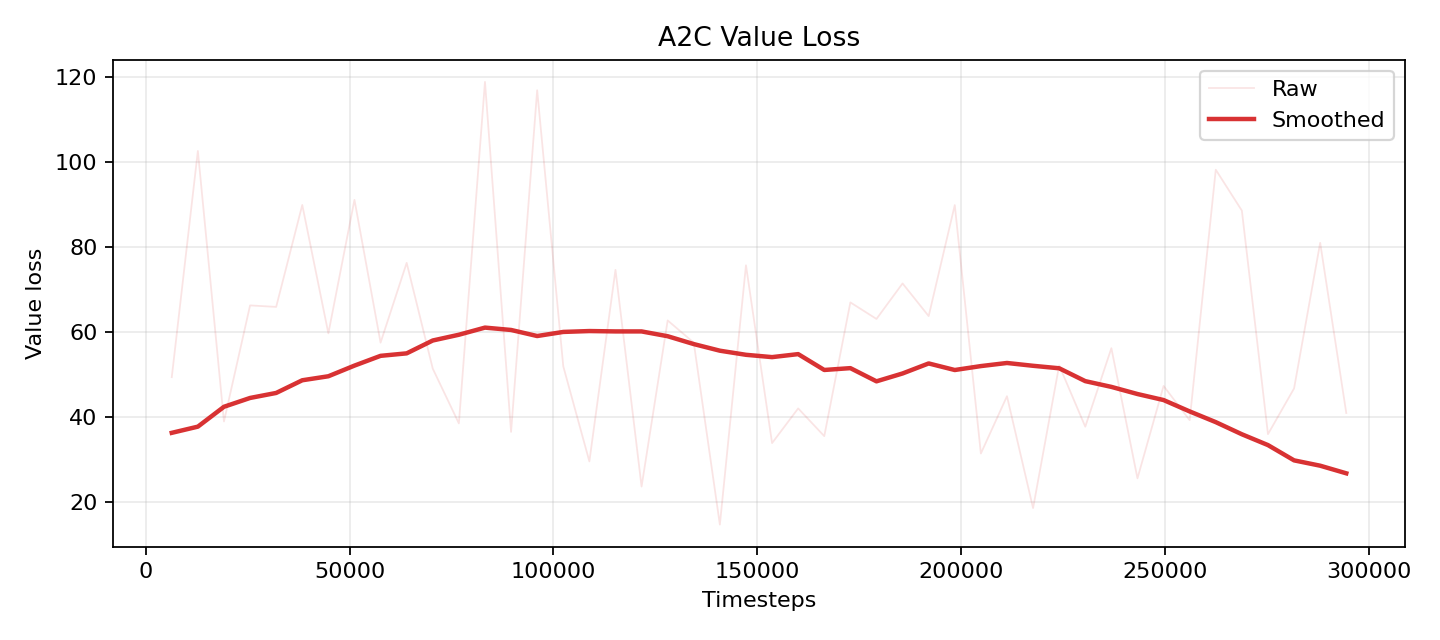
\includegraphics[width=0.9\textwidth]{graphics/chapter-6/train_A2C/value_loss_curve.png}
    \captionsetup{hypcap=false}
    \captionof{figure}{Biến thiên \textit{value loss} của A2C}
    \label{fig:a2c-value-loss}
\end{minipage}

\noindent Hình \ref{fig:a2c-value-loss} biểu diễn biến thiên của hàm mất mát giá trị (\textit{value loss}) phản ánh sai số dự báo phần thưởng tích lũy của Critic. Hàm mất mát này ban đầu tăng từ 36 lên đỉnh điểm quanh mức 60 tại 100\,000 bước do tác nhân liên tục khám phá các trạng thái mới chưa có trong bộ nhớ. Sau khi mạng Critic học được xấp xỉ giá trị trạng thái tốt hơn, \textit{value loss} giảm dần về mức dưới 30 ở cuối quá trình huấn luyện, cho thấy chất lượng đánh giá trạng thái ngày càng chính xác.

\begin{minipage}{\textwidth}
    \centering
    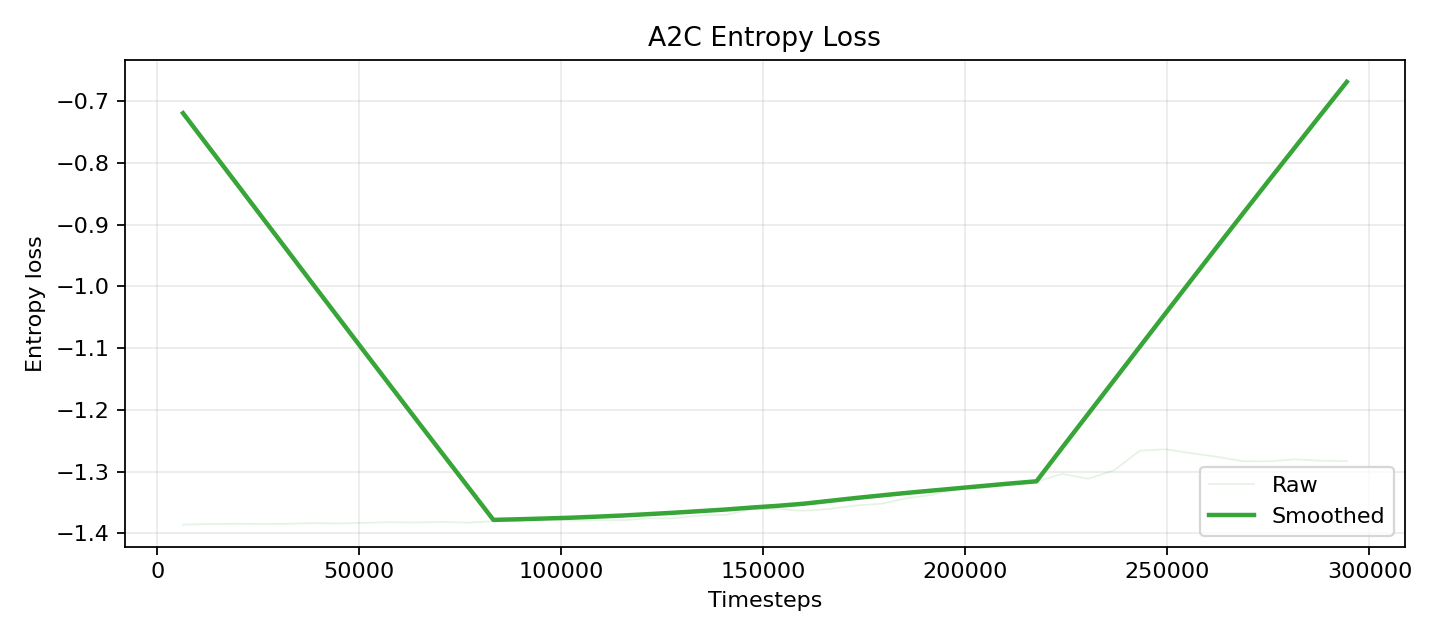
\includegraphics[width=0.9\textwidth]{graphics/chapter-6/train_A2C/entropy_curve.png}
    \captionsetup{hypcap=false}
    \captionof{figure}{Biến thiên \textit{entropy loss} của A2C}
    \label{fig:a2c-entropy-loss}
\end{minipage}

\noindent Ở Hình \ref{fig:a2c-entropy-loss}, tổn thất entropy (\textit{entropy loss}) bắt đầu từ mức -0.72 và giảm mạnh xuống -1.38 trong 80\,000 bước đầu, cho thấy chính sách đang dần tập trung vào các hành động có độ tin cậy cao. Sau 220\,000 bước, entropy loss lại có xu hướng tăng trở lại lên mức -0.67, điều này phản ánh việc điều chỉnh chính sách hoặc ảnh hưởng từ tốc độ học (learning rate) giúp tác nhân tăng cường thăm dò trở lại để tránh hội tụ vào các cực trị địa phương kém tối ưu.

\begin{minipage}{\textwidth}
    \centering
    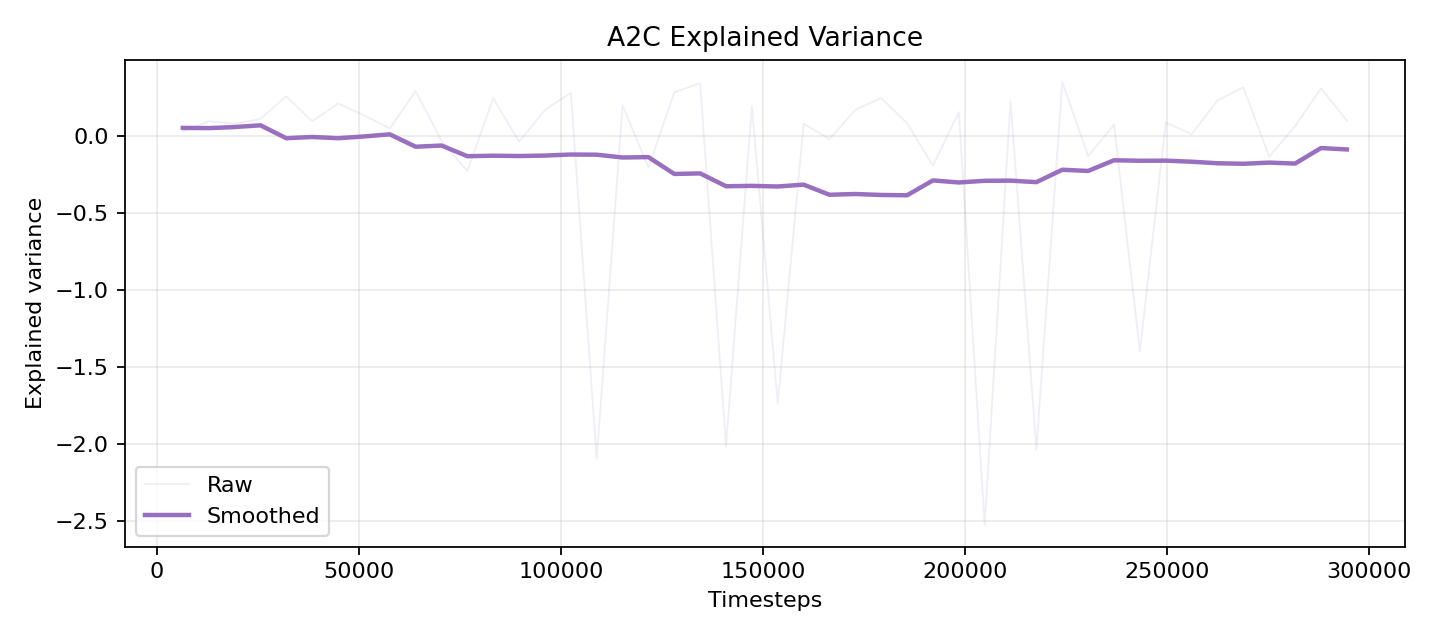
\includegraphics[width=0.92\textwidth]{graphics/chapter-6/train_A2C/explained_variance_curve.png}
    \captionsetup{hypcap=false}
    \captionof{figure}{Biến thiên sai số giải thích (\textit{explained variance}) của A2C}
    \label{fig:a2c-explained-variance}
\end{minipage}

\noindent Chỉ số phương sai giải thích (\textit{explained variance}) được biểu diễn trong Hình \ref{fig:a2c-explained-variance}. Chỉ số này đo lường mức độ dự báo chính xác của Critic đối với sự biến thiên phần thưởng. Giá trị \textit{explained variance} dao động chủ yếu trong khoảng từ 0.0 đến -0.4, phản ánh đặc trưng khó khăn trong việc dự đoán chính xác giá trị trạng thái trên môi trường có nhiễu động cao của hệ thống microservices.

\begin{minipage}{\textwidth}
    \centering
    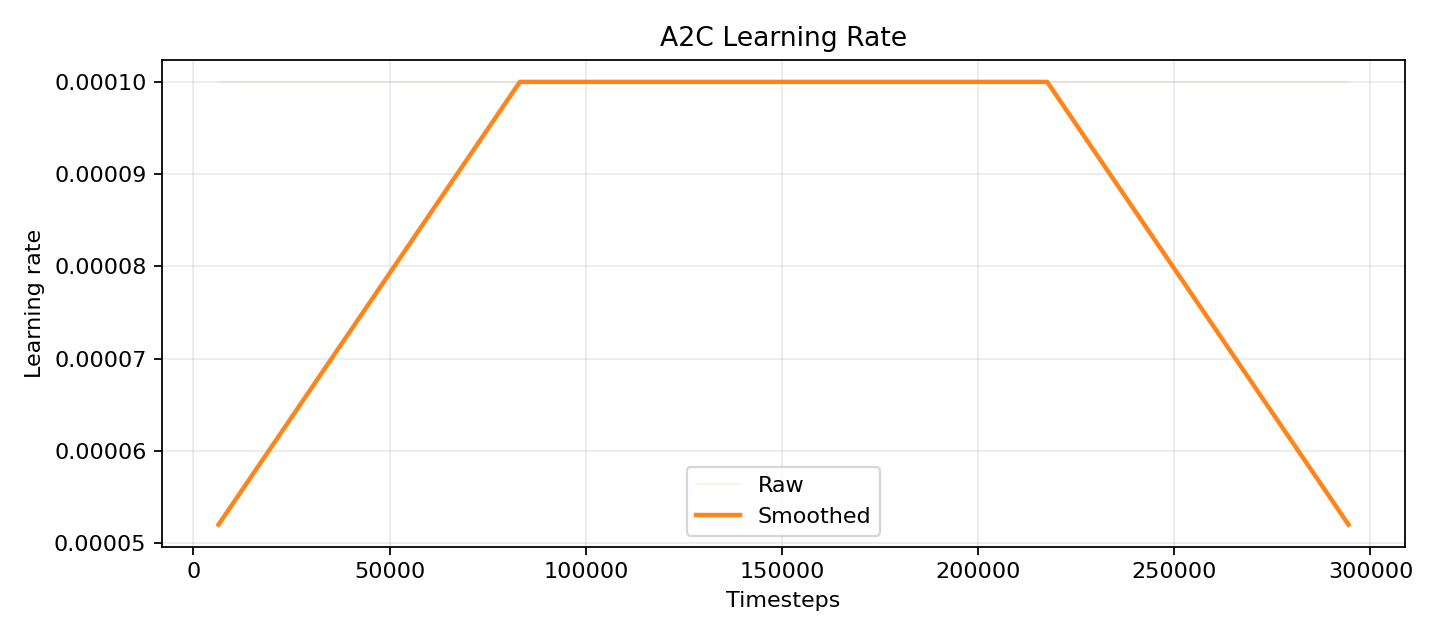
\includegraphics[width=0.9\textwidth]{graphics/chapter-6/train_A2C/learning_rate_curve.png}
    \captionsetup{hypcap=false}
    \captionof{figure}{Biến thiên tốc độ học trong quá trình huấn luyện A2C}
    \label{fig:a2c-learning-rate}
\end{minipage}

\noindent Hình \ref{fig:a2c-learning-rate} mô tả lịch trình thay đổi tốc độ học (\textit{learning rate}) của A2C. Tốc độ học được thiết lập tăng dần từ $5\times10^{-5}$ lên $10^{-4}$ trong 80\,000 bước đầu tiên để khởi động quá trình tối ưu hóa (warmup), duy trì ổn định đến bước thứ 220\,000, sau đó giảm dần về mức ban đầu ở bước thứ 300\,000 (cooldown). Lịch trình này giúp mô hình ổn định các bước đi gradient ở cả hai giai đoạn đầu và cuối huấn luyện.

\begin{minipage}{\textwidth}
    \centering
    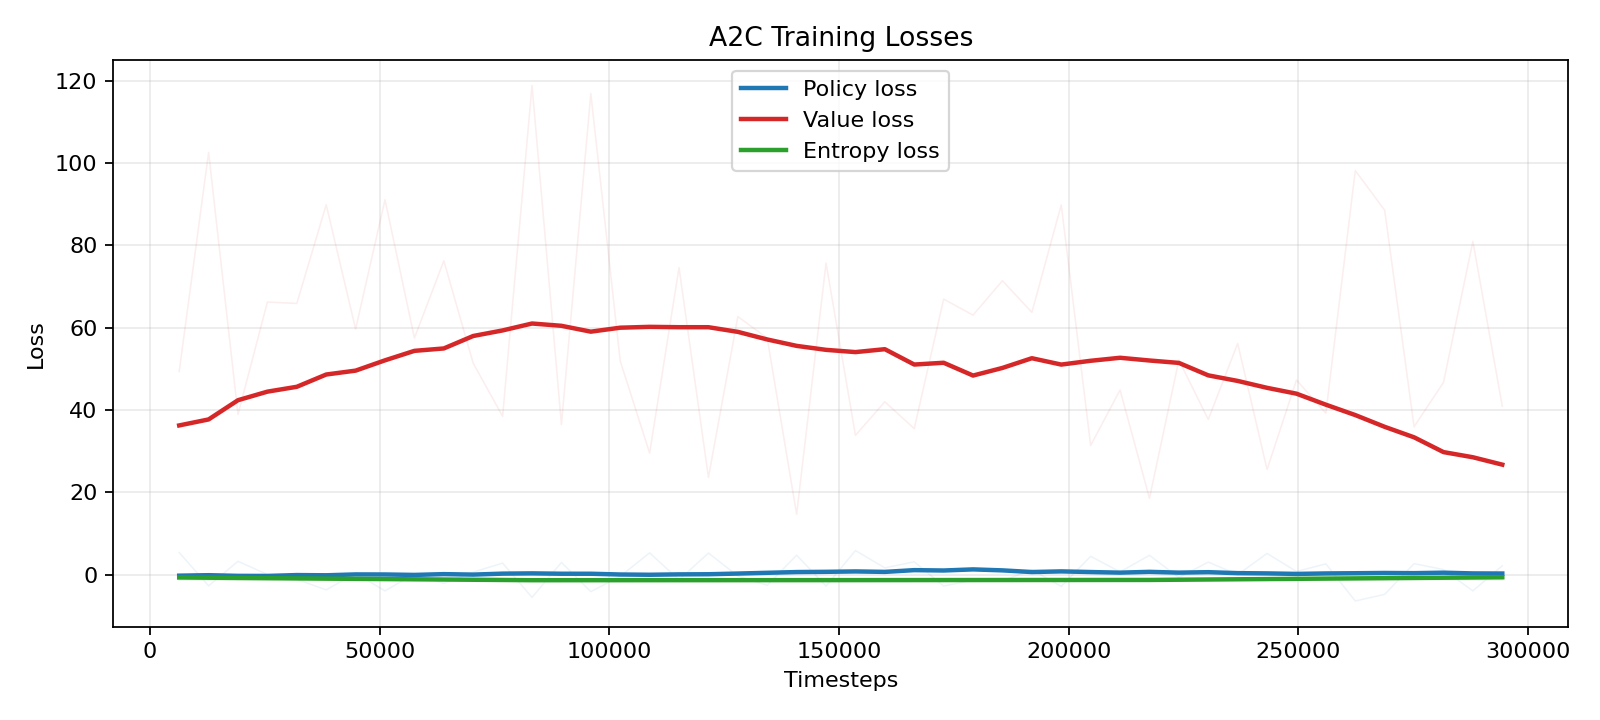
\includegraphics[width=0.92\textwidth]{graphics/chapter-6/train_A2C/loss_curve.png}
    \captionsetup{hypcap=false}
    \captionof{figure}{Biểu đồ tổng hợp các hàm mất mát chính của A2C}
    \label{fig:a2c-loss-summary}
\end{minipage}

\noindent Hình \ref{fig:a2c-loss-summary} tổng hợp đồng thời cả ba thành phần loss chính của thuật toán A2C. Biểu đồ cho thấy \textit{value loss} chiếm tỷ trọng lớn nhất về mặt thang đo, trong khi \textit{policy loss} và \textit{entropy loss} duy trì mức dao động nhỏ và ổn định xung quanh 0, đảm bảo tiến trình học song song của Actor và Critic diễn ra cân bằng.

\begin{minipage}{\textwidth}
    \centering
    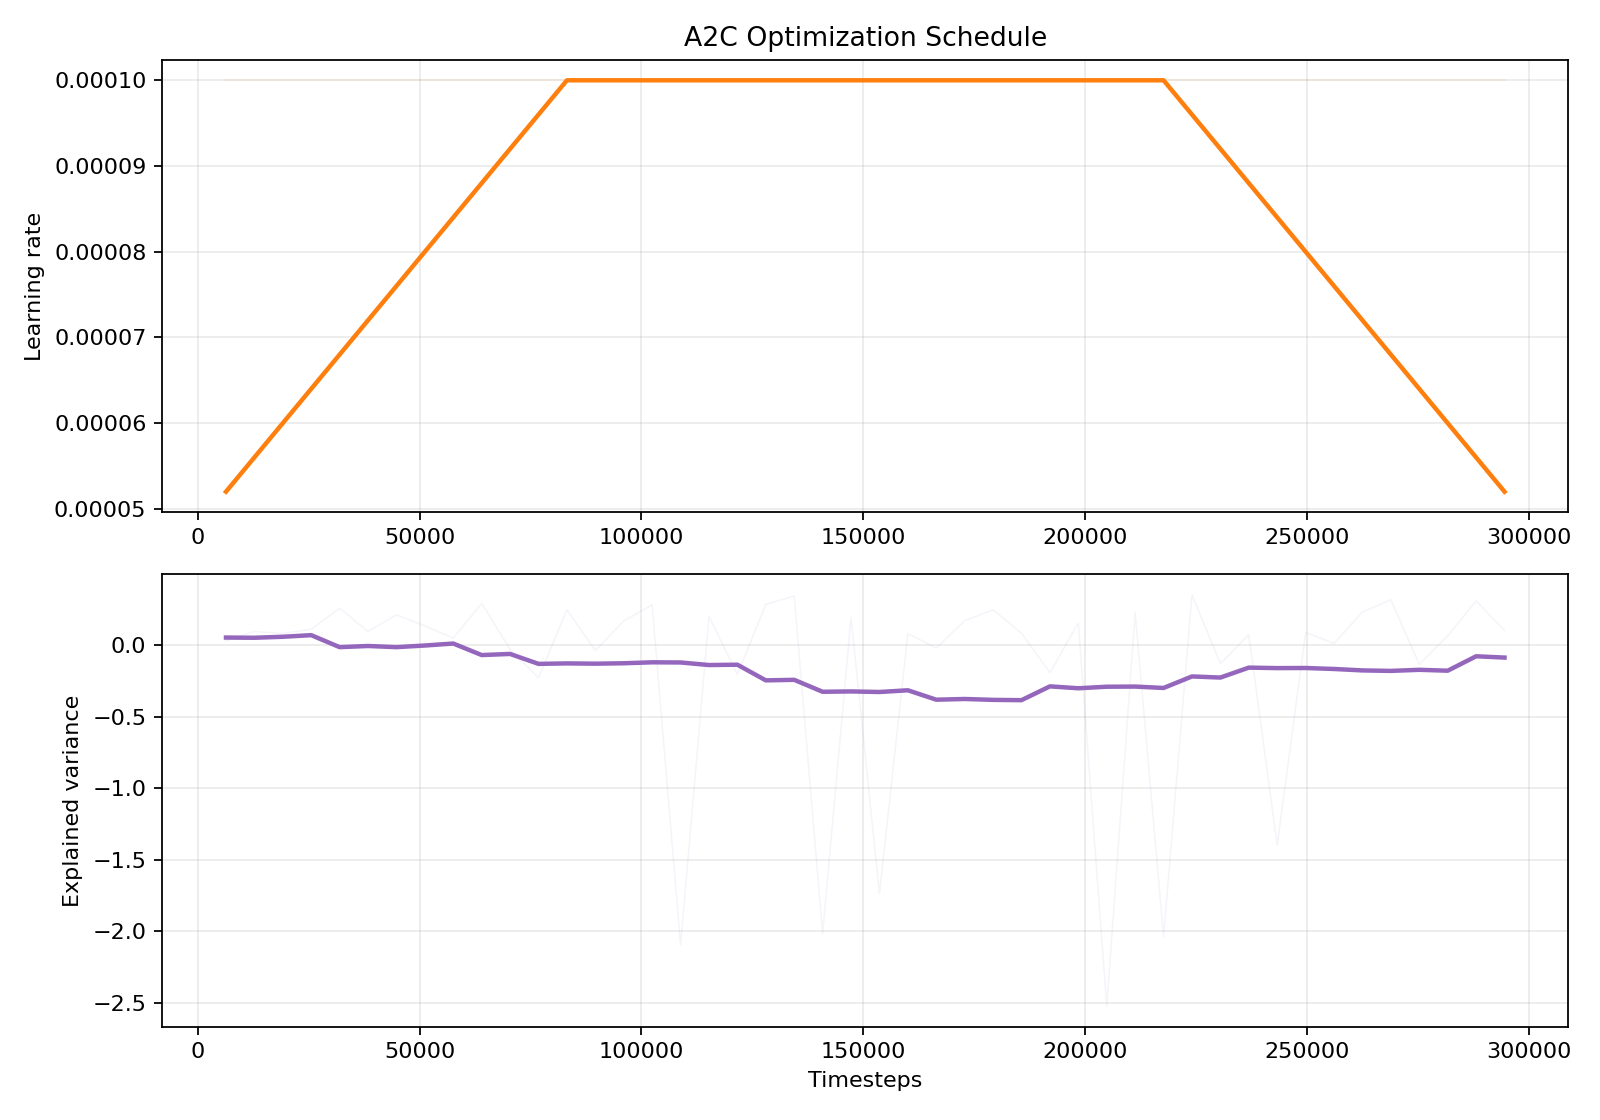
\includegraphics[width=0.92\textwidth]{graphics/chapter-6/train_A2C/optimization_curve.png}
    \captionsetup{hypcap=false}
    \captionof{figure}{Biểu đồ tổng hợp lịch tối ưu hóa của A2C}
    \label{fig:a2c-optimization-summary}
\end{minipage}

\noindent Hình \ref{fig:a2c-optimization-summary} tổng hợp lịch trình tốc độ học và sai số giải thích của A2C. Sự đối chiếu này cho thấy mối tương quan rõ rệt giữa việc thay đổi tốc độ học và tính ổn định của các chỉ số chẩn đoán tối ưu hóa.

\begin{minipage}{\textwidth}
    \centering
    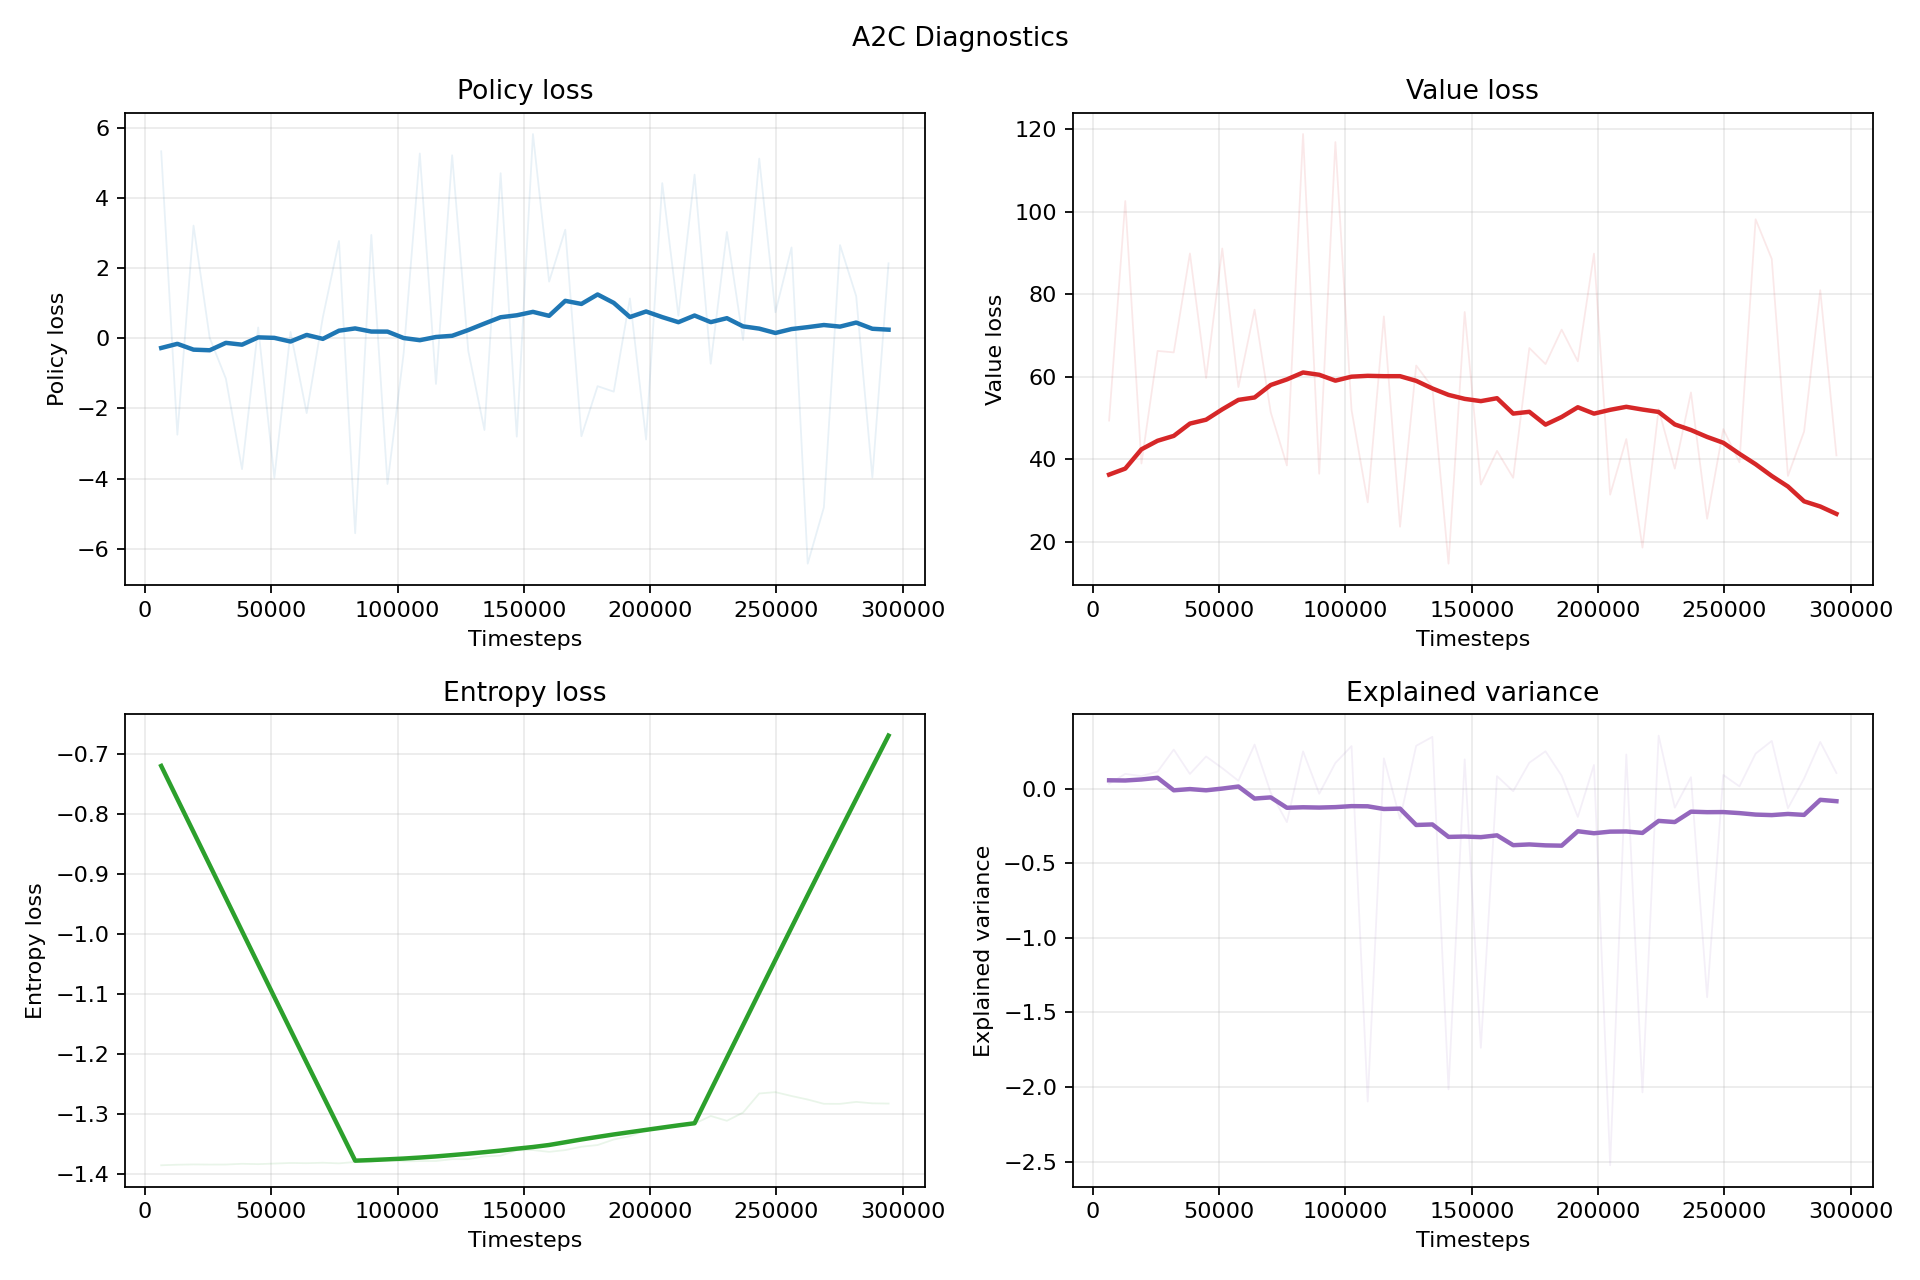
\includegraphics[width=0.92\textwidth]{graphics/chapter-6/train_A2C/a2c_diagnostics.png}
    \captionsetup{hypcap=false}
    \captionof{figure}{Biểu đồ chẩn đoán tổng hợp của A2C}
    \label{fig:a2c-diagnostics-summary}
\end{minipage}

\noindent Toàn bộ các thông số chẩn đoán huấn luyện của A2C được tổng hợp trực quan trong Hình \ref{fig:a2c-diagnostics-summary}. Sự nhất quán của cả bốn đồ thị thành phần khẳng định tiến trình học của A2C diễn ra ổn định và an toàn.

\begin{minipage}{\textwidth}
    \centering
    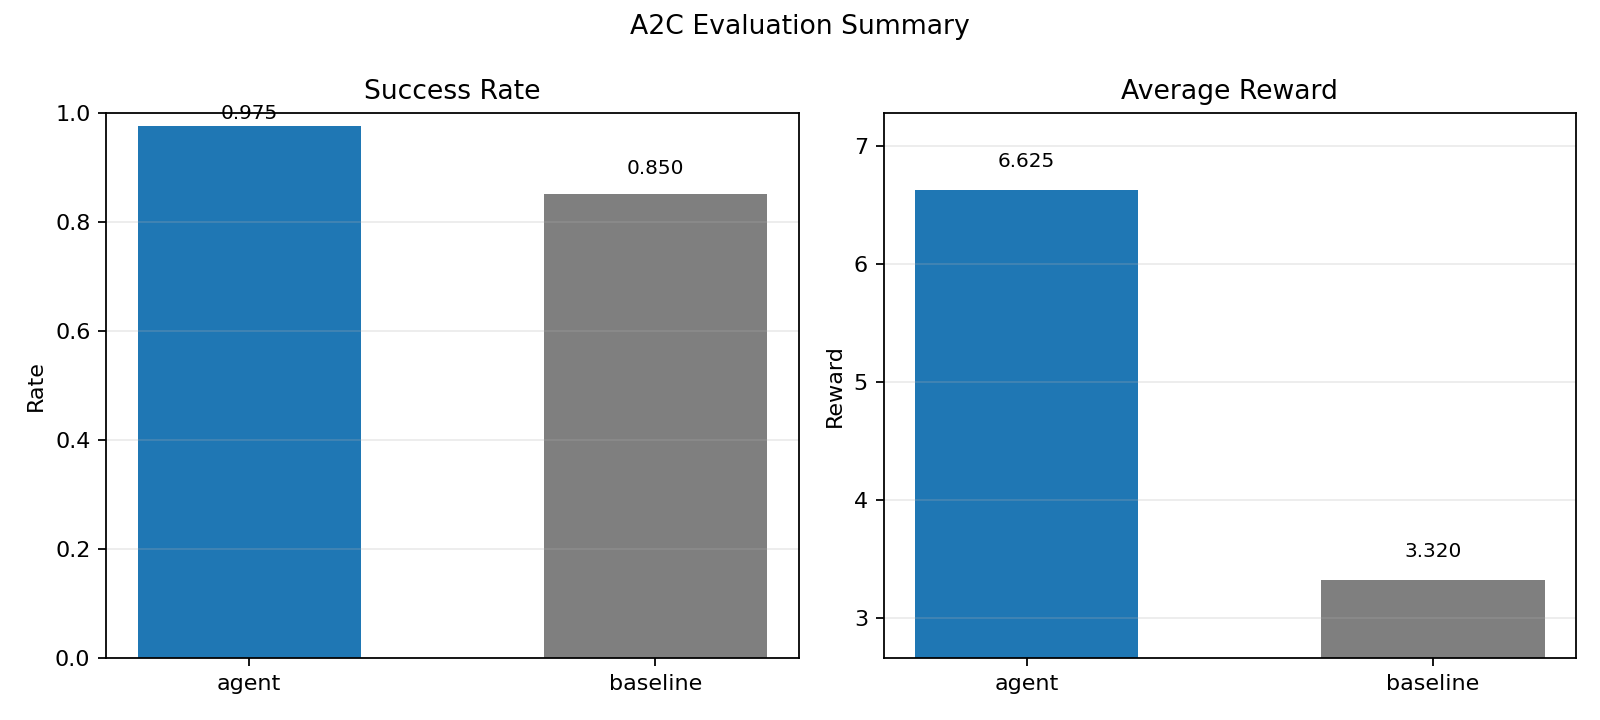
\includegraphics[width=0.92\textwidth]{graphics/chapter-6/train_A2C/evaluation_summary.png}
    \captionsetup{hypcap=false}
    \captionof{figure}{So sánh kết quả đánh giá A2C với baseline}
    \label{fig:a2c-evaluation-summary}
\end{minipage}

\noindent Kết quả đánh giá trong Hình \ref{fig:a2c-evaluation-summary} so sánh hiệu năng của tác nhân A2C sau huấn luyện với baseline ngẫu nhiên. Kết quả cho thấy tác nhân A2C đạt tỷ lệ phục hồi thành công vượt trội lên tới 0.975 (so với 0.850 của baseline). Đồng thời, phần thưởng trung bình đạt 6.625, cao gấp đôi so với mức 3.320 của baseline. Sự cải thiện vượt bậc này chứng minh tính hiệu quả của chính sách Actor-Critic trong việc tự phục hồi hệ thống khi xảy ra sự cố pod.


\subsection{PPO}

Đối với PPO, run huấn luyện được theo dõi trong khoảng 400\,000 bước thời gian. Trọng tâm của phần này là quan sát mức độ hội tụ của chính sách, độ ổn định của các đại lượng tối ưu hóa và kết quả đánh giá sau huấn luyện trên kịch bản \textit{pod failure}.

\begin{minipage}{\textwidth}
    \centering
    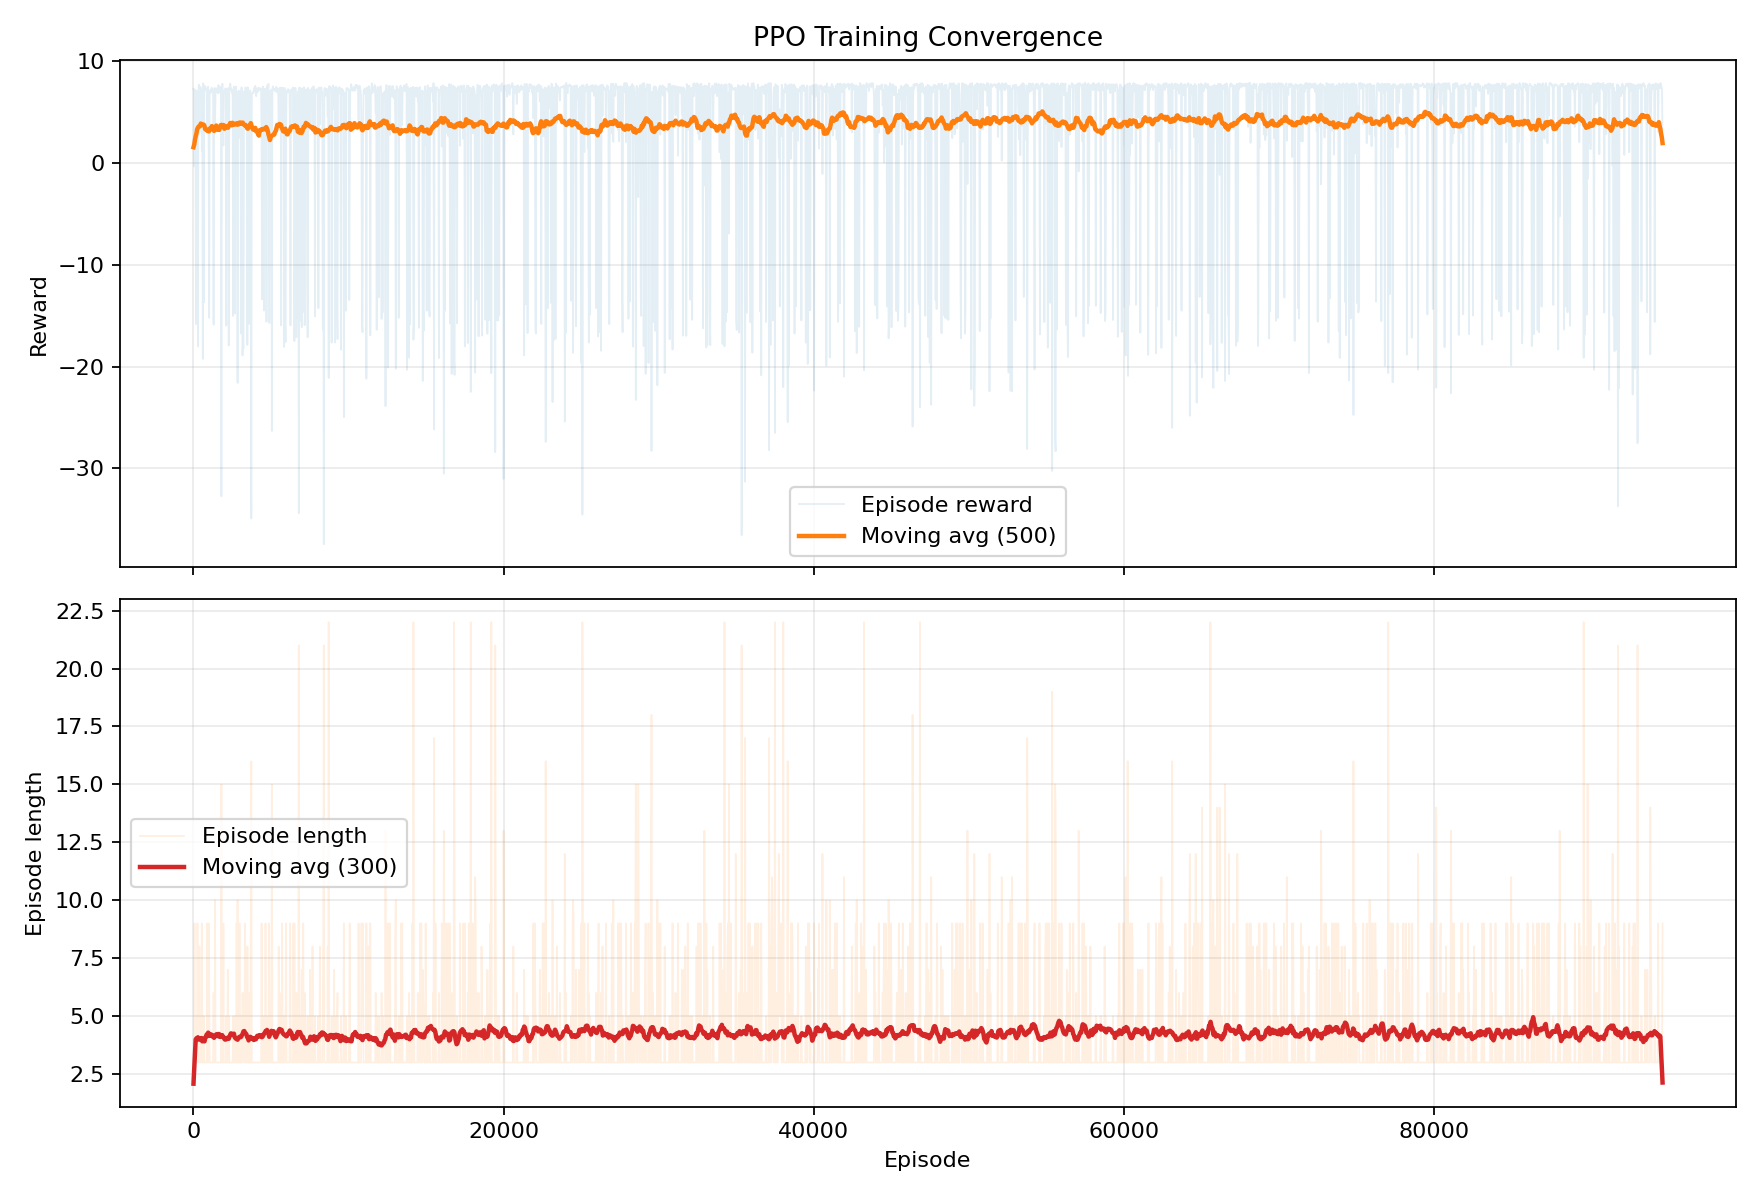
\includegraphics[width=0.95\textwidth]{graphics/chapter-6/train_PPO/training_curve.png}
    \captionsetup{hypcap=false}
    \captionof{figure}{Biểu đồ hội tụ theo phần thưởng và độ dài episode của PPO}
    \label{fig:ppo-training-convergence}
\end{minipage}

\noindent Hình \ref{fig:ppo-training-convergence} cho thấy phần thưởng theo episode có độ dao động lớn ở mức tức thời, phản ánh đúng bản chất nhiễu của môi trường replay từ dữ liệu thật. Tuy nhiên, đường trung bình trượt của phần thưởng duy trì xu hướng dương và tăng dần từ khoảng 3 lên trên 4, cho thấy chính sách PPO học được hành vi phục hồi ngày càng hiệu quả hơn. Ở đồ thị độ dài episode, giá trị trung bình ổn định quanh 4--5 bước, nghĩa là tác nhân thường đưa hệ thống về trạng thái phục hồi trong số bước tương đối ngắn.

\begin{minipage}{\textwidth}
    \centering
    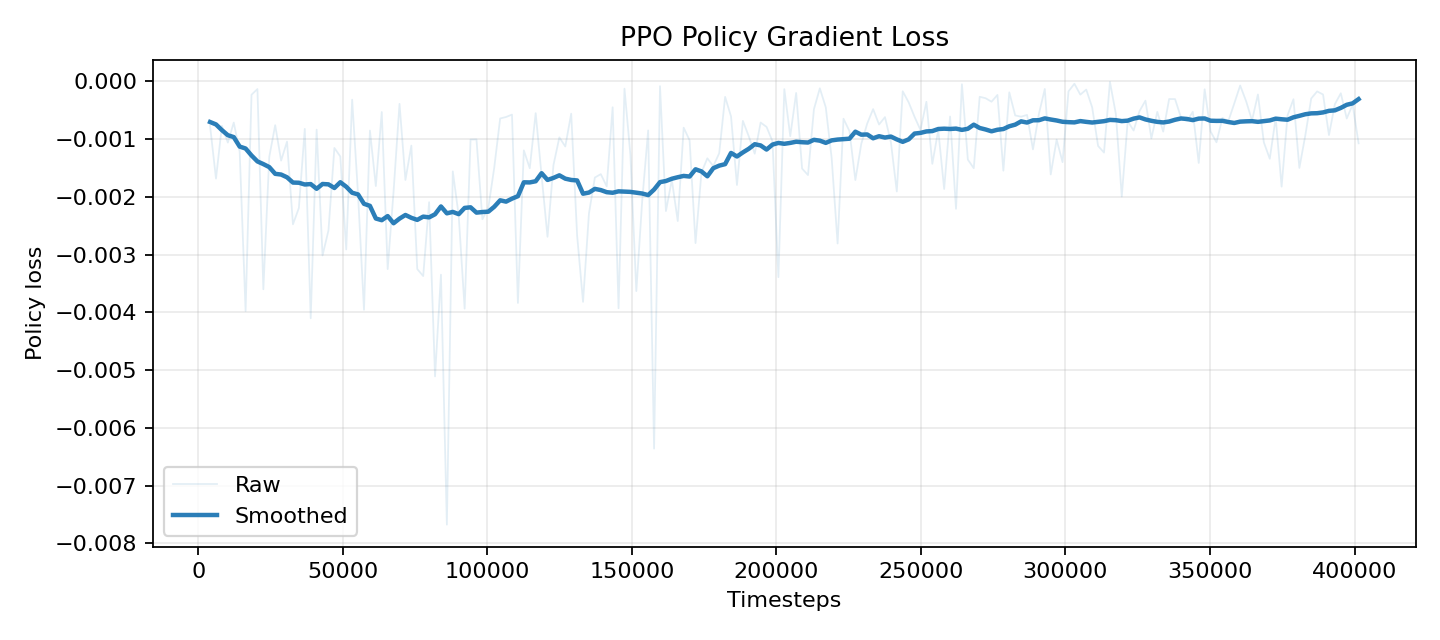
\includegraphics[width=0.9\textwidth]{graphics/chapter-6/train_PPO/policy_loss_curve.png}
    \captionsetup{hypcap=false}
    \captionof{figure}{Biến thiên \textit{policy loss} trong quá trình huấn luyện PPO}
    \label{fig:ppo-policy-loss}
\end{minipage}

\noindent Với Hình \ref{fig:ppo-policy-loss}, \textit{policy loss} ban đầu giảm xuống mức âm lớn hơn về độ lớn, sau đó tăng dần trở lại gần 0. Diễn biến này cho thấy ở giai đoạn đầu, chính sách thay đổi mạnh để nhanh chóng thích nghi với dữ liệu huấn luyện; về sau, độ lớn cập nhật giảm đi, phản ánh việc chính sách đã ổn định hơn và chỉ còn tinh chỉnh cục bộ.

\begin{minipage}{\textwidth}
    \centering
    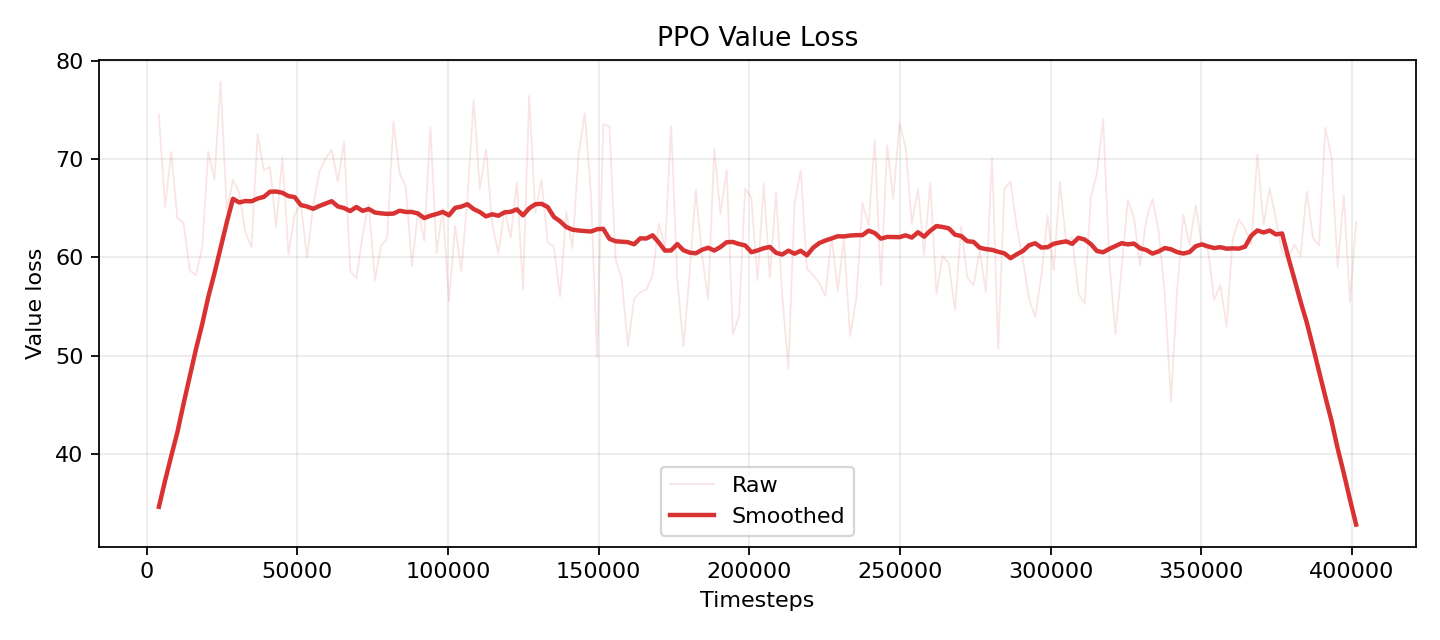
\includegraphics[width=0.9\textwidth]{graphics/chapter-6/train_PPO/value_loss_curve.png}
    \captionsetup{hypcap=false}
    \captionof{figure}{Biến thiên \textit{value loss} của PPO}
    \label{fig:ppo-value-loss}
\end{minipage}

\noindent Hình \ref{fig:ppo-value-loss} cho thấy \textit{value loss} dao động chủ yếu trong vùng 60--66 sau giai đoạn khởi đầu. Mặc dù vẫn còn nhiễu theo từng lần cập nhật, đường làm mượt không có xu hướng bùng nổ, qua đó cho thấy mạng giá trị giữ được sự ổn định trong suốt quá trình học. Phần giảm mạnh ở cuối đồ thị chủ yếu mang tính biên của đường làm mượt, vì vậy không nên diễn giải như một bước nhảy chất lượng đột ngột.

\begin{minipage}{\textwidth}
    \centering
    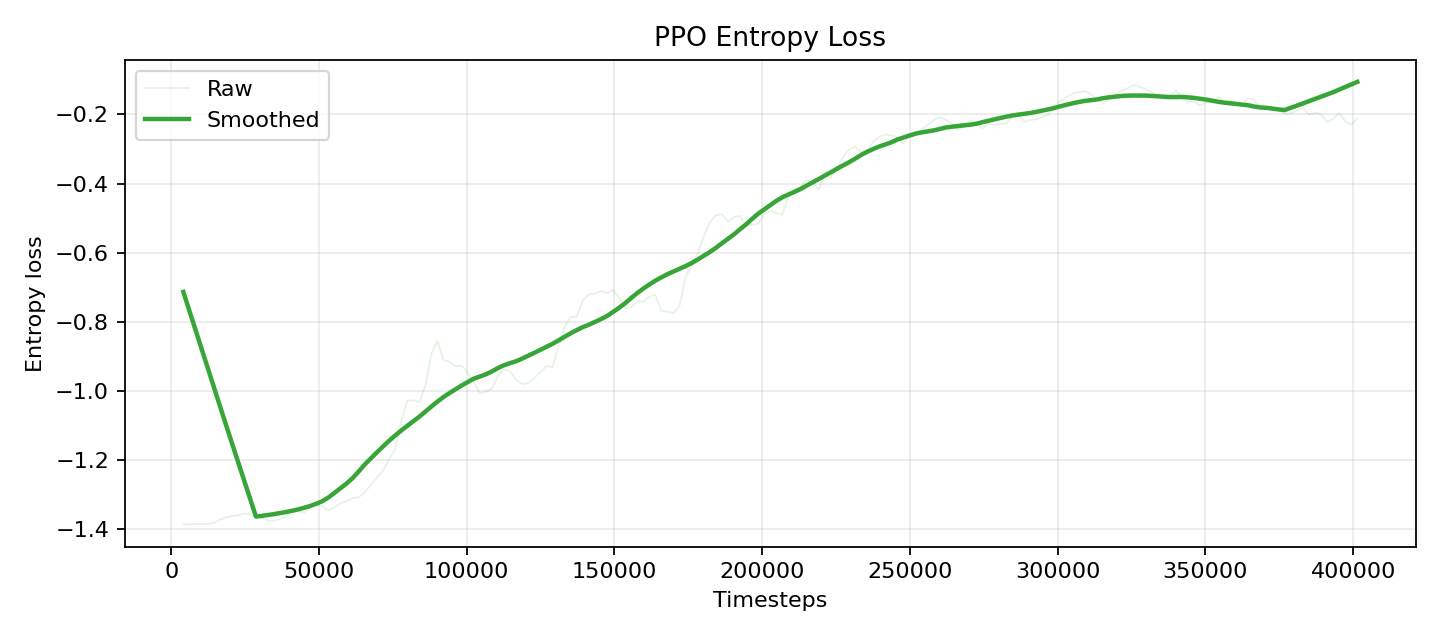
\includegraphics[width=0.9\textwidth]{graphics/chapter-6/train_PPO/entropy_curve.png}
    \captionsetup{hypcap=false}
    \captionof{figure}{Biến thiên \textit{entropy loss} của PPO}
    \label{fig:ppo-entropy-loss}
\end{minipage}

\noindent Ở Hình \ref{fig:ppo-entropy-loss}, \textit{entropy loss} dịch dần từ vùng âm lớn về gần 0. Điều này phản ánh entropy của chính sách giảm theo thời gian, tức là tác nhân bớt ngẫu nhiên hơn và ngày càng tập trung vào một tập hành động phục hồi nhất quán. Đây là tín hiệu tích cực, vì nó cho thấy PPO không chỉ học được mà còn dần củng cố một chính sách có tính quyết đoán hơn.

\begin{minipage}{\textwidth}
    \centering
    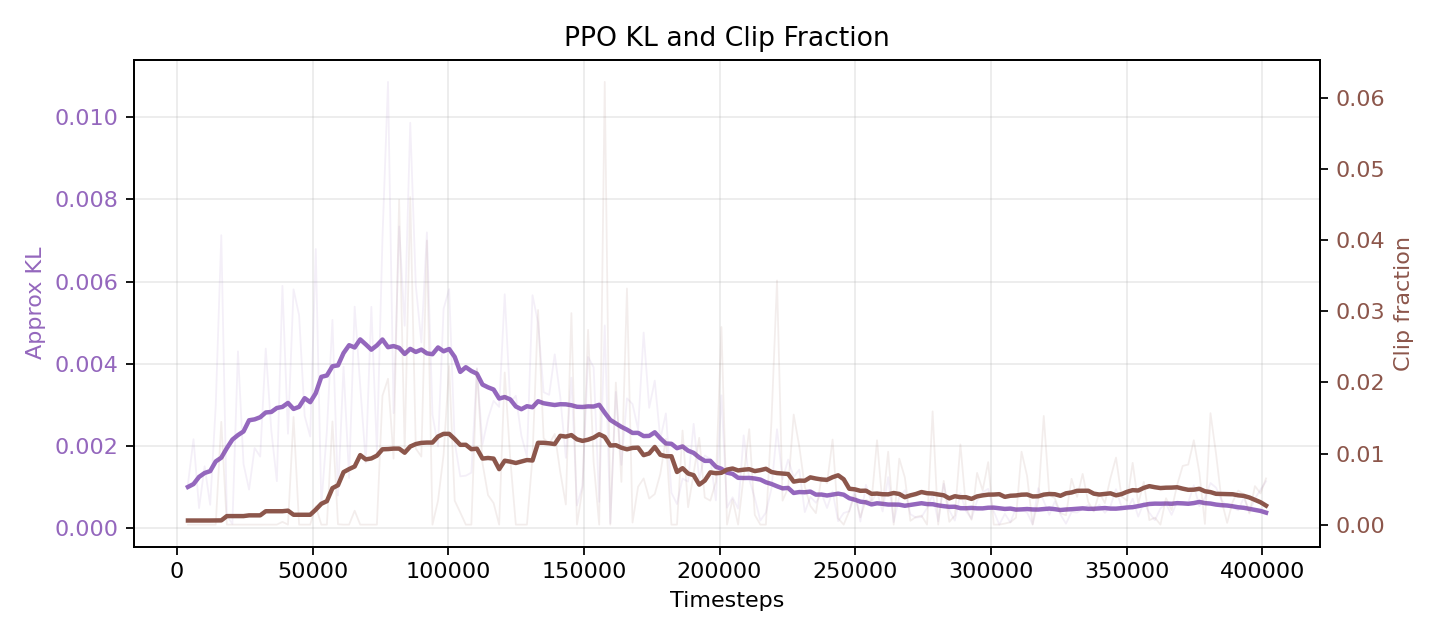
\includegraphics[width=0.92\textwidth]{graphics/chapter-6/train_PPO/kl_clip_curve.png}
    \captionsetup{hypcap=false}
    \captionof{figure}{Độ lệch KL xấp xỉ và \textit{clip fraction} trong PPO}
    \label{fig:ppo-kl-clip}
\end{minipage}

\noindent Hình \ref{fig:ppo-kl-clip} cho thấy \textit{approx KL} tăng dần ở giai đoạn đầu và đạt đỉnh khoảng 0.004--0.005 trước khi giảm về mức rất thấp ở cuối quá trình. Đồng thời, \textit{clip fraction} chỉ dao động quanh vùng nhỏ và cũng giảm dần sau nửa sau của quá trình học. Hai tín hiệu này cho thấy các bước cập nhật chính sách được kiểm soát tốt, không vượt quá ngưỡng thay đổi lớn và phù hợp với đặc trưng tối ưu hóa ổn định của PPO.

\begin{minipage}{\textwidth}
    \centering
    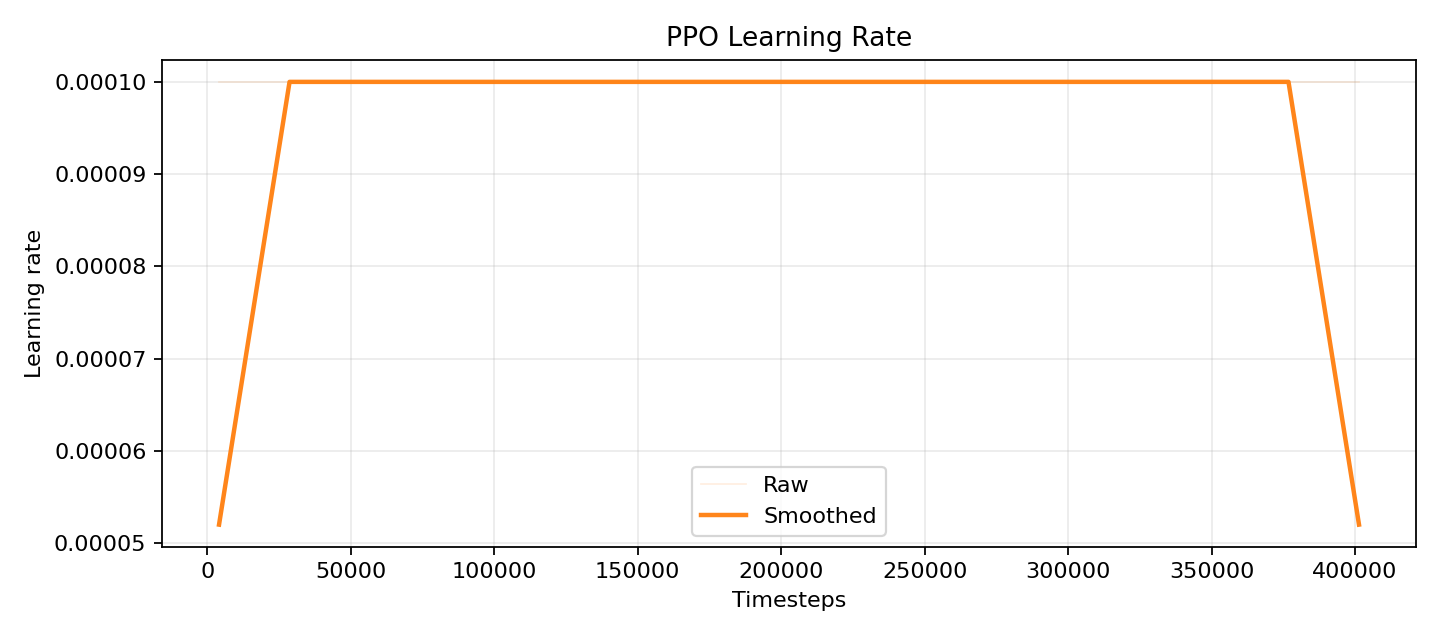
\includegraphics[width=0.9\textwidth]{graphics/chapter-6/train_PPO/learning_rate_curve.png}
    \captionsetup{hypcap=false}
    \captionof{figure}{Biến thiên tốc độ học trong quá trình huấn luyện PPO}
    \label{fig:ppo-learning-rate}
\end{minipage}

\noindent Từ Hình \ref{fig:ppo-learning-rate}, có thể thấy tốc độ học được duy trì gần như cố định quanh mức $10^{-4}$ trong phần lớn thời gian huấn luyện. Việc giữ \textit{learning rate} ổn định giúp PPO tránh được dao động tối ưu hóa quá mạnh, đồng thời tạo điều kiện để các chỉ số \textit{policy loss}, \textit{value loss} và \textit{approx KL} hội tụ theo hướng mượt hơn.

\begin{minipage}{\textwidth}
    \centering
    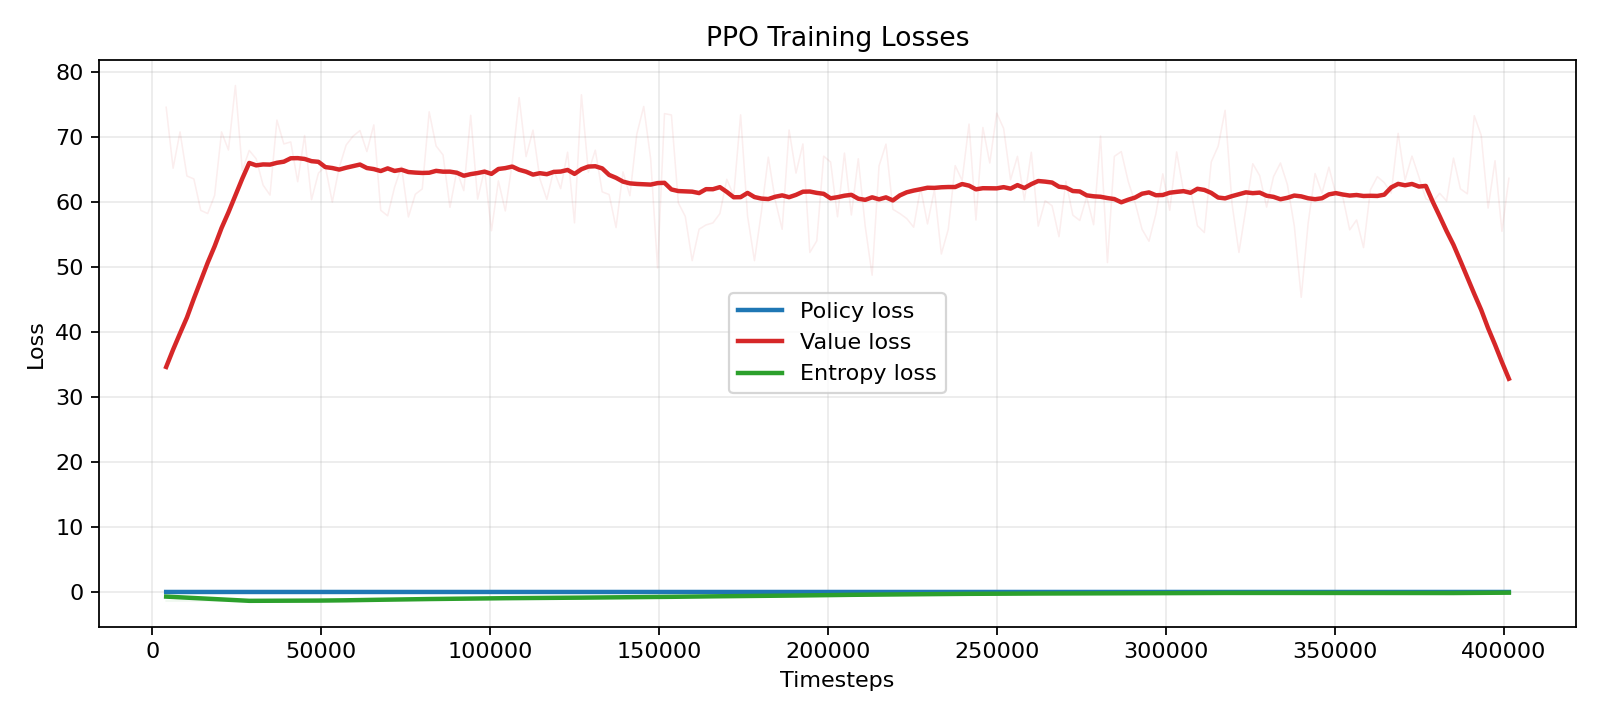
\includegraphics[width=0.92\textwidth]{graphics/chapter-6/train_PPO/loss_curve.png}
    \captionsetup{hypcap=false}
    \captionof{figure}{Biểu đồ tổng hợp các hàm mất mát chính của PPO}
    \label{fig:ppo-loss-summary}
\end{minipage}

\noindent Hình \ref{fig:ppo-loss-summary} tổng hợp đồng thời \textit{policy loss}, \textit{value loss} và \textit{entropy loss}. Có thể thấy \textit{value loss} chiếm thang đo lớn nhất, trong khi hai thành phần còn lại dao động nhỏ hơn nhiều. Dù khác thang đo, ba đại lượng đều giữ xu hướng ổn định theo thời gian và không xuất hiện hiện tượng phân kỳ, cho thấy quá trình học của actor và critic vẫn được duy trì cân bằng.

\begin{minipage}{\textwidth}
    \centering
    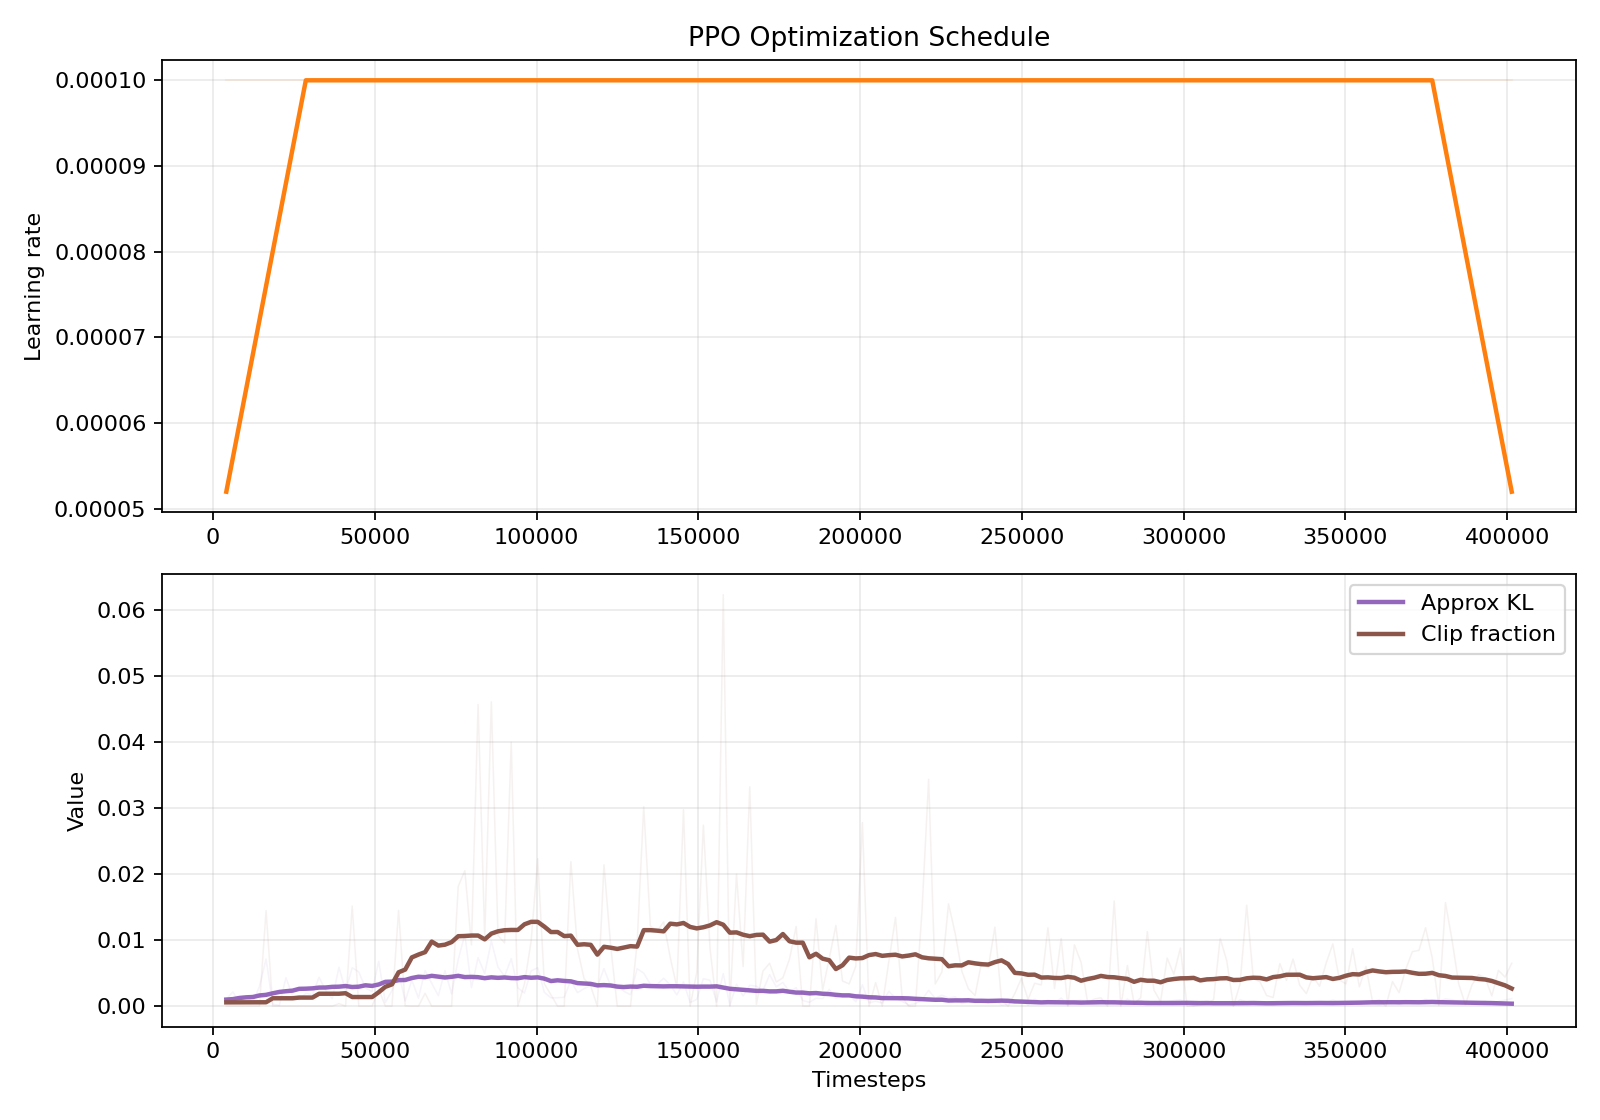
\includegraphics[width=0.92\textwidth]{graphics/chapter-6/train_PPO/optimization_curve.png}
    \captionsetup{hypcap=false}
    \captionof{figure}{Biểu đồ tổng hợp lịch tối ưu hóa và mức độ cập nhật chính sách của PPO}
    \label{fig:ppo-optimization-summary}
\end{minipage}

\noindent Hình \ref{fig:ppo-optimization-summary} cho thấy lại mối quan hệ giữa lịch tốc độ học, \textit{approx KL} và \textit{clip fraction} trong cùng một khung nhìn. Kết quả nhất quán với các đồ thị trước: tốc độ học ổn định, độ lệch KL được giữ nhỏ, và tỷ lệ bị clip không tăng đột biến. Điều này củng cố nhận định rằng PPO cập nhật chính sách theo hướng an toàn, phù hợp với bài toán yêu cầu hạn chế can thiệp quá mức lên hệ thống thật.

\begin{minipage}{\textwidth}
    \centering
    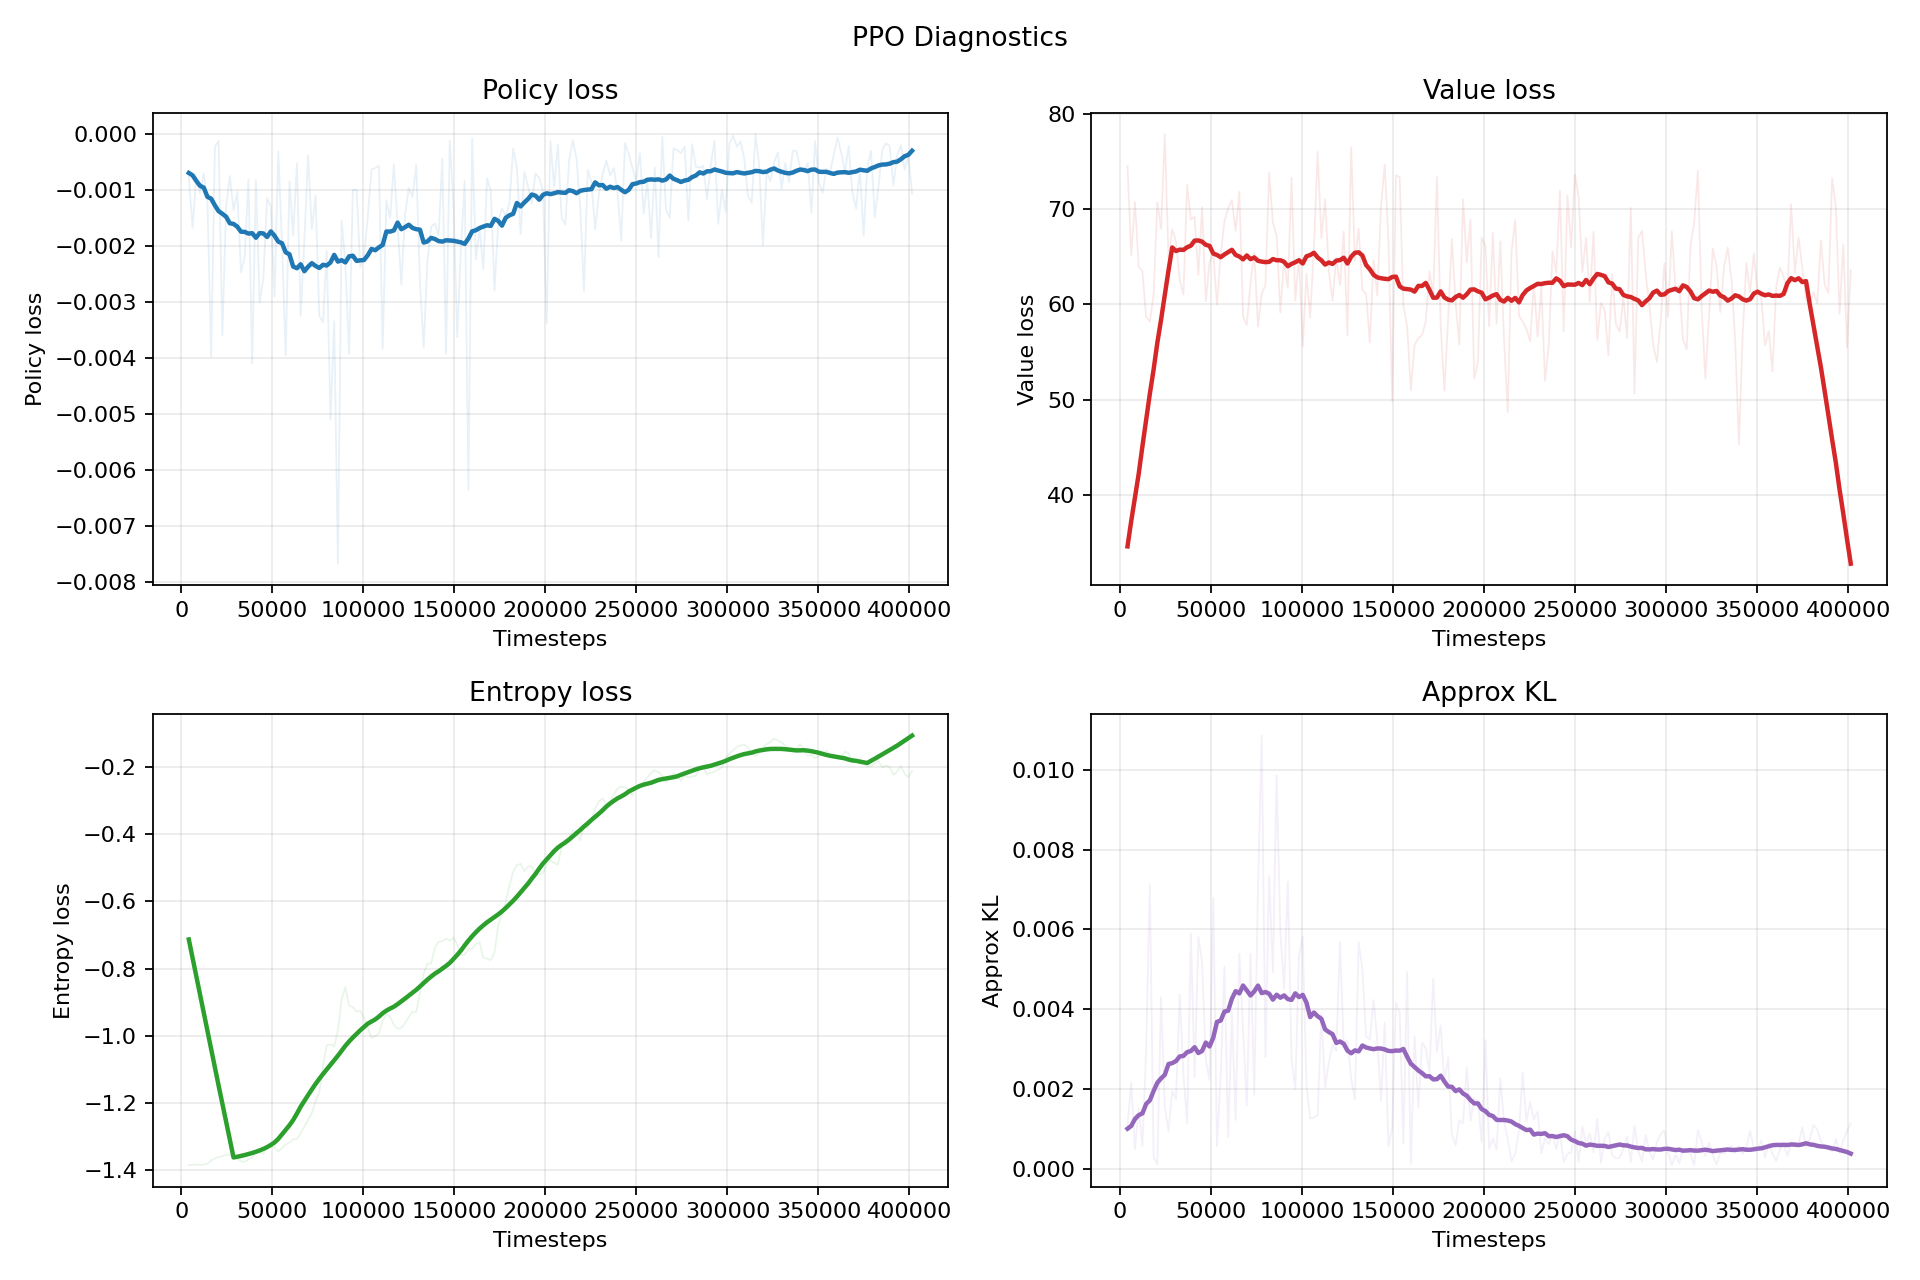
\includegraphics[width=0.92\textwidth]{graphics/chapter-6/train_PPO/ppo_diagnostics.png}
    \captionsetup{hypcap=false}
    \captionof{figure}{Biểu đồ chẩn đoán tổng hợp của PPO}
    \label{fig:ppo-diagnostics-summary}
\end{minipage}

\noindent Hình \ref{fig:ppo-diagnostics-summary} đóng vai trò đối chiếu nhanh toàn bộ các tín hiệu chẩn đoán quan trọng của PPO trong một trang duy nhất. Bốn đồ thị thành phần cùng chỉ ra một kết luận nhất quán: chính sách được cải thiện mạnh ở nửa đầu quá trình học, sau đó chuyển sang pha tinh chỉnh ổn định hơn ở nửa sau.

\begin{minipage}{\textwidth}
    \centering
    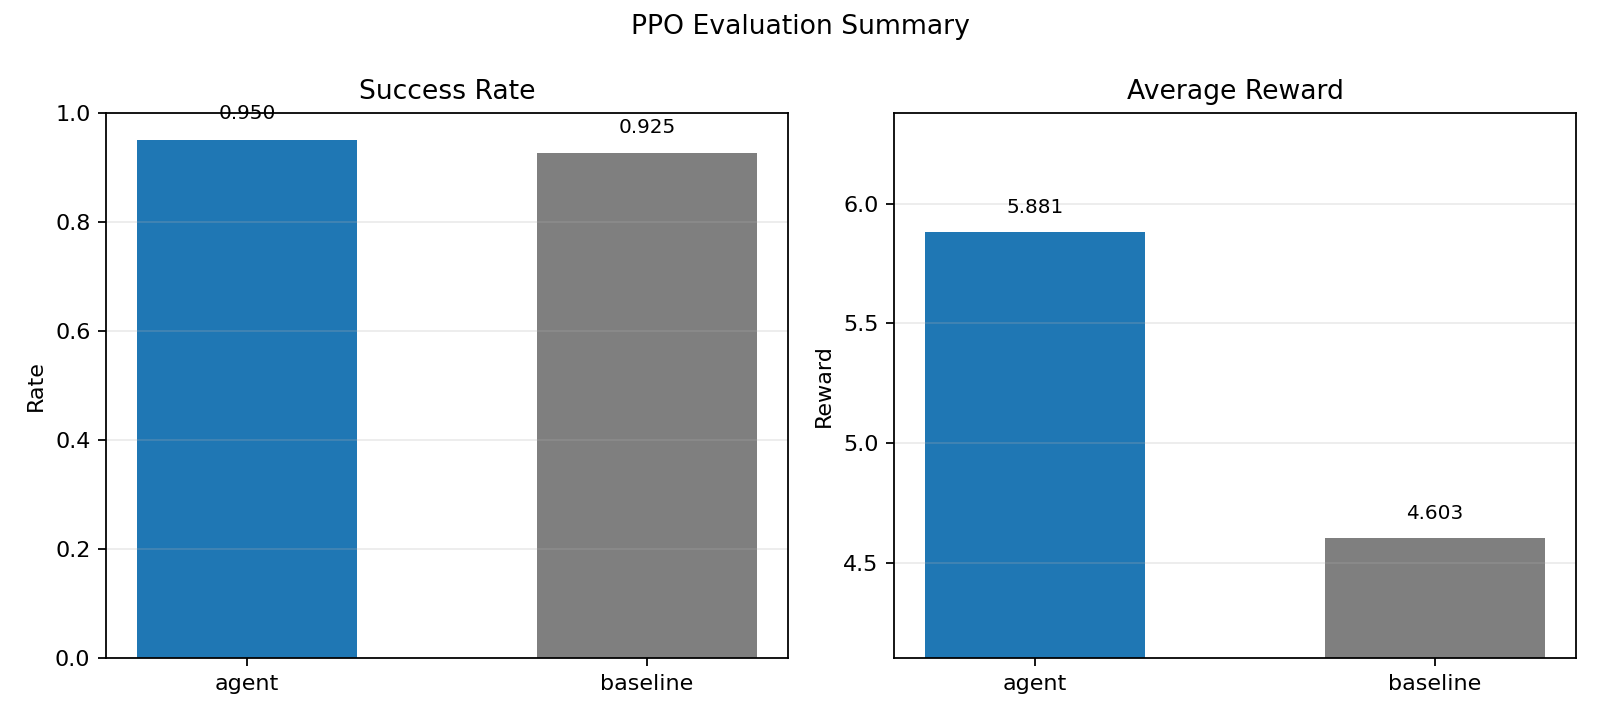
\includegraphics[width=0.92\textwidth]{graphics/chapter-6/train_PPO/evaluation_summary.png}
    \captionsetup{hypcap=false}
    \captionof{figure}{So sánh kết quả đánh giá PPO với baseline}
    \label{fig:ppo-evaluation-summary}
\end{minipage}

\noindent Tổng hợp các kết quả trên, PPO cho thấy ba đặc điểm tích cực trên kịch bản \textit{pod failure}: (i) đường phần thưởng hội tụ theo xu hướng tăng, (ii) các đại lượng tối ưu hóa như \textit{KL}, \textit{clip fraction} và các hàm mất mát được giữ trong miền ổn định, và (iii) kết quả đánh giá cuối cùng tốt hơn baseline cả về \textit{success rate} lẫn phần thưởng trung bình. Vì vậy, trong phạm vi thực nghiệm hiện tại, PPO là một ứng viên phù hợp cho bài toán tự phục hồi Kubernetes dựa trên học tăng cường.


\section{So sánh kết quả đánh giá offline giữa các thuật toán}

\noindent Sau khi hoàn thành giai đoạn huấn luyện riêng cho từng mô hình, nhóm tiến hành đánh giá offline trên cùng tập episode của kịch bản \textit{pod failure} để đối chiếu trực tiếp giữa DQN, A2C, PPO và baseline. Mục tiêu của phần này là xem xét không chỉ tỷ lệ phục hồi thành công, mà còn cả chất lượng hành vi can thiệp, độ dài chuỗi phục hồi và tác động của từng chính sách lên các chỉ số hệ thống quan trọng.

\begin{minipage}{\textwidth}
    \centering
    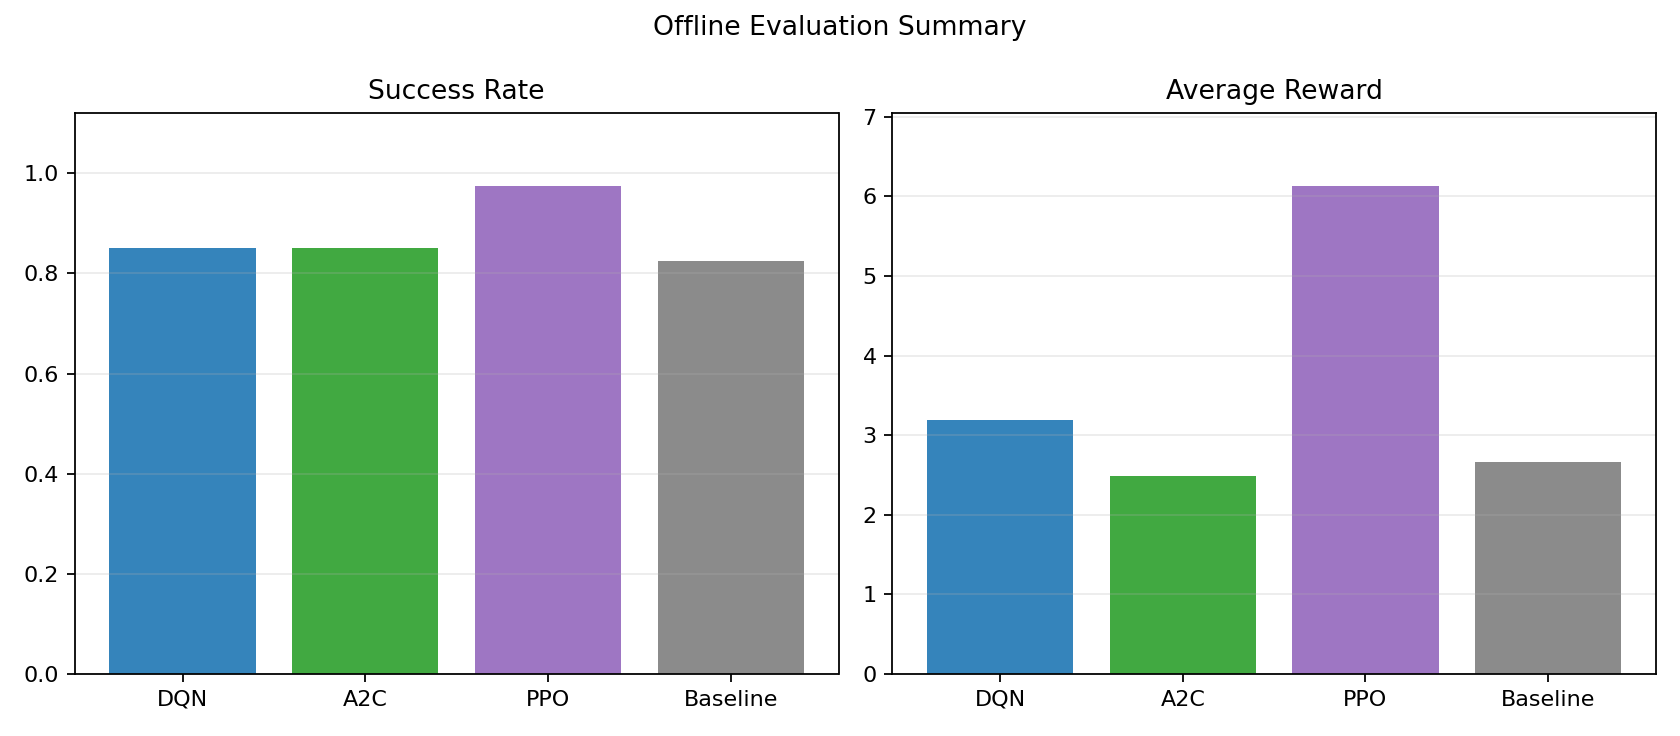
\includegraphics[width=0.92\textwidth]{graphics/chapter-6/compare/evaluation_summary.png}
    \captionsetup{hypcap=false}
    \captionof{figure}{Kết quả đánh giá offline tổng hợp của các thuật toán}
    \label{fig:compare-evaluation-summary}
\end{minipage}

\noindent Hình \ref{fig:compare-evaluation-summary} trình bày hai đại lượng tổng quát nhất của pha đánh giá offline là \textit{success rate} và \textit{average reward}. Có thể thấy PPO đạt kết quả nổi bật nhất với tỷ lệ thành công xấp xỉ 0.97 và phần thưởng trung bình trên 6.0. Trong khi đó, DQN và A2C cùng đạt mức \textit{success rate} khoảng 0.85, đều cao hơn baseline khoảng 0.82. Xét theo phần thưởng trung bình, DQN đạt khoảng 3.2, baseline khoảng 2.6 và A2C khoảng 2.5. Kết quả này cho thấy PPO không chỉ phục hồi thành công với tần suất cao hơn mà còn tạo ra chuỗi hành động có chất lượng tốt hơn theo đúng hàm thưởng đã thiết kế.

\begin{minipage}{\textwidth}
    \centering
    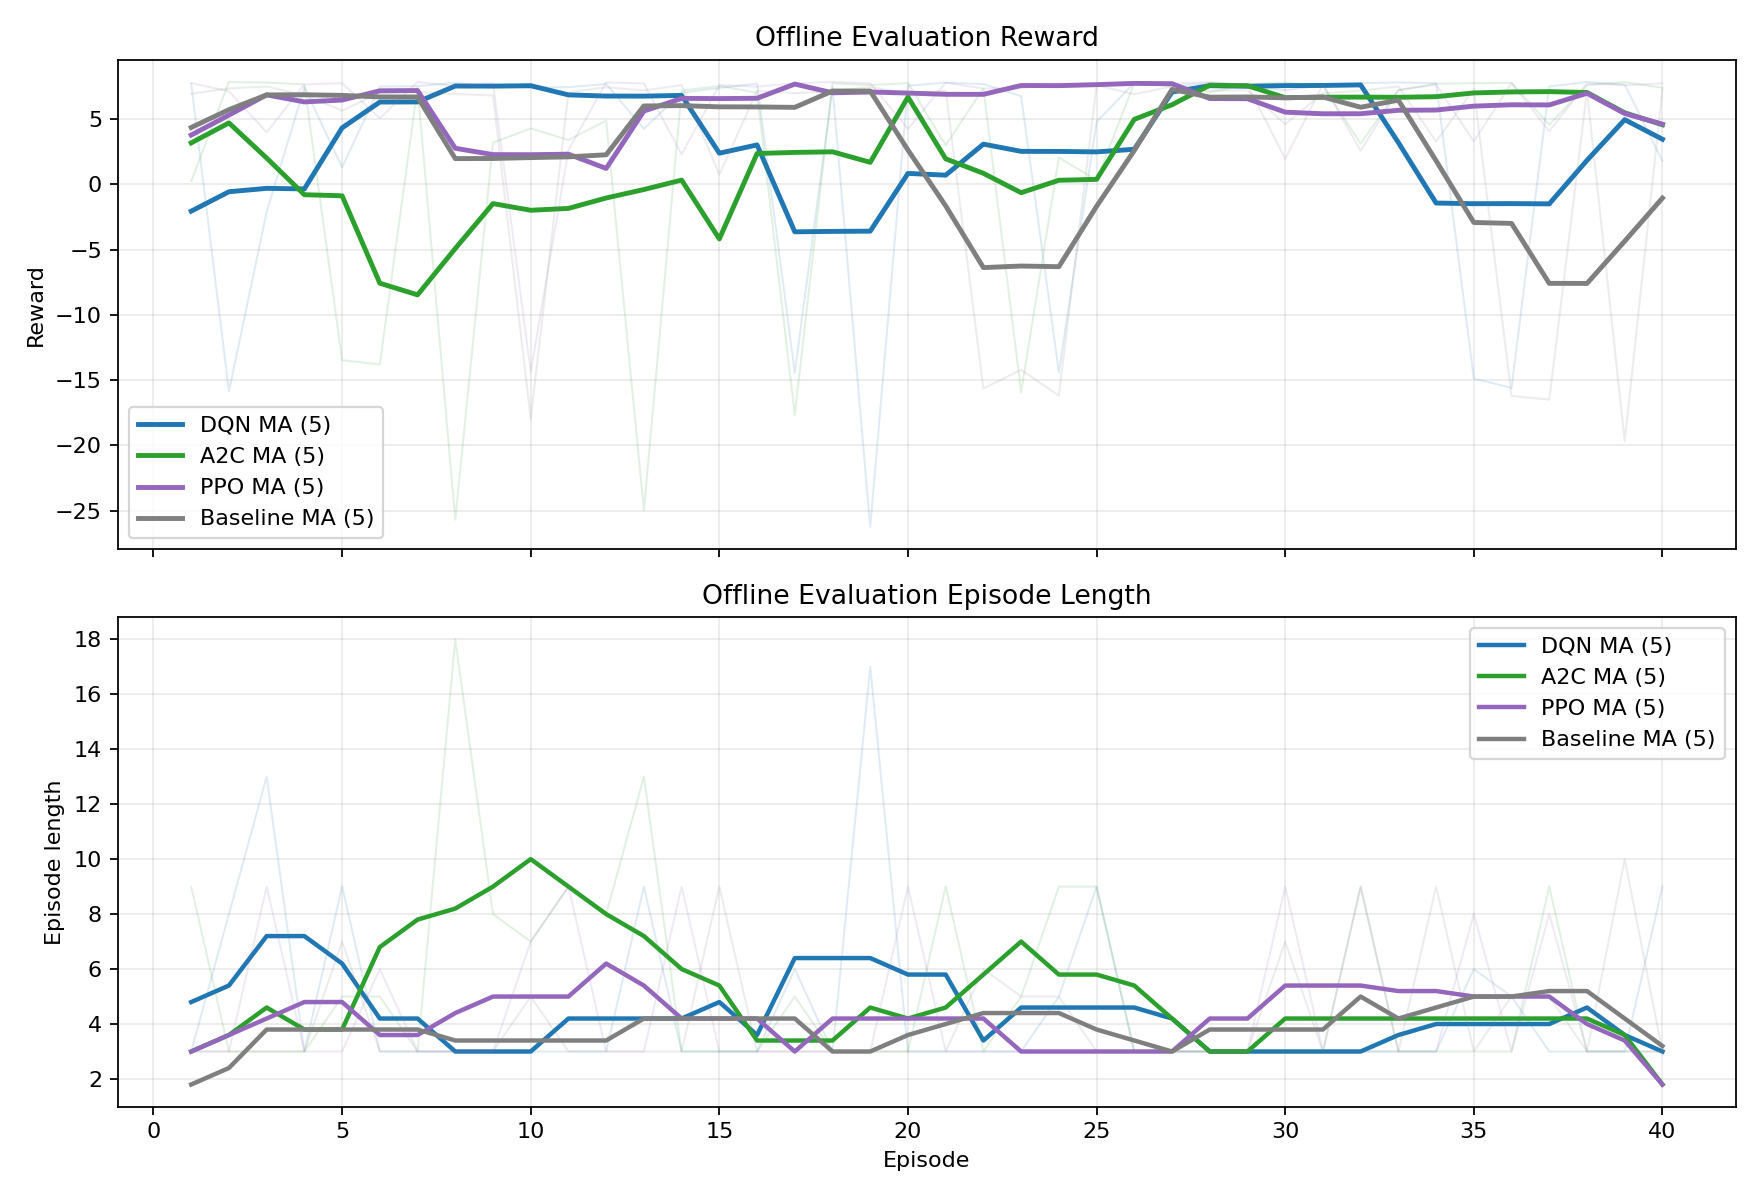
\includegraphics[width=0.95\textwidth]{graphics/chapter-6/compare/episode_curves.png}
    \captionsetup{hypcap=false}
    \captionof{figure}{Biến thiên phần thưởng và độ dài episode trong các tập đánh giá}
    \label{fig:compare-episode-curves}
\end{minipage}

\noindent Diễn biến chi tiết theo từng episode được thể hiện trong Hình \ref{fig:compare-episode-curves}. Đường trung bình trượt MA(5) của PPO duy trì ở vùng cao và ổn định nhất trong cả hai khía cạnh: phần thưởng thường nằm trong vùng dương cao, còn độ dài episode chủ yếu dao động quanh 3--5 bước. DQN cho kết quả trung bình khá hơn baseline nhưng vẫn xuất hiện một số đoạn giảm reward rõ rệt ở các episode khó. A2C có giai đoạn reward giảm sâu hơn DQN và PPO, đồng thời độ dài episode biến động mạnh hơn ở nửa đầu tập đánh giá. Nhìn chung, biểu đồ này củng cố nhận định rằng PPO có độ ổn định tốt nhất khi đối mặt với nhiều quỹ đạo lỗi khác nhau, trong khi DQN đứng ở vị trí trung gian và A2C nhạy hơn với các episode bất lợi.

\begin{minipage}{\textwidth}
    \centering
    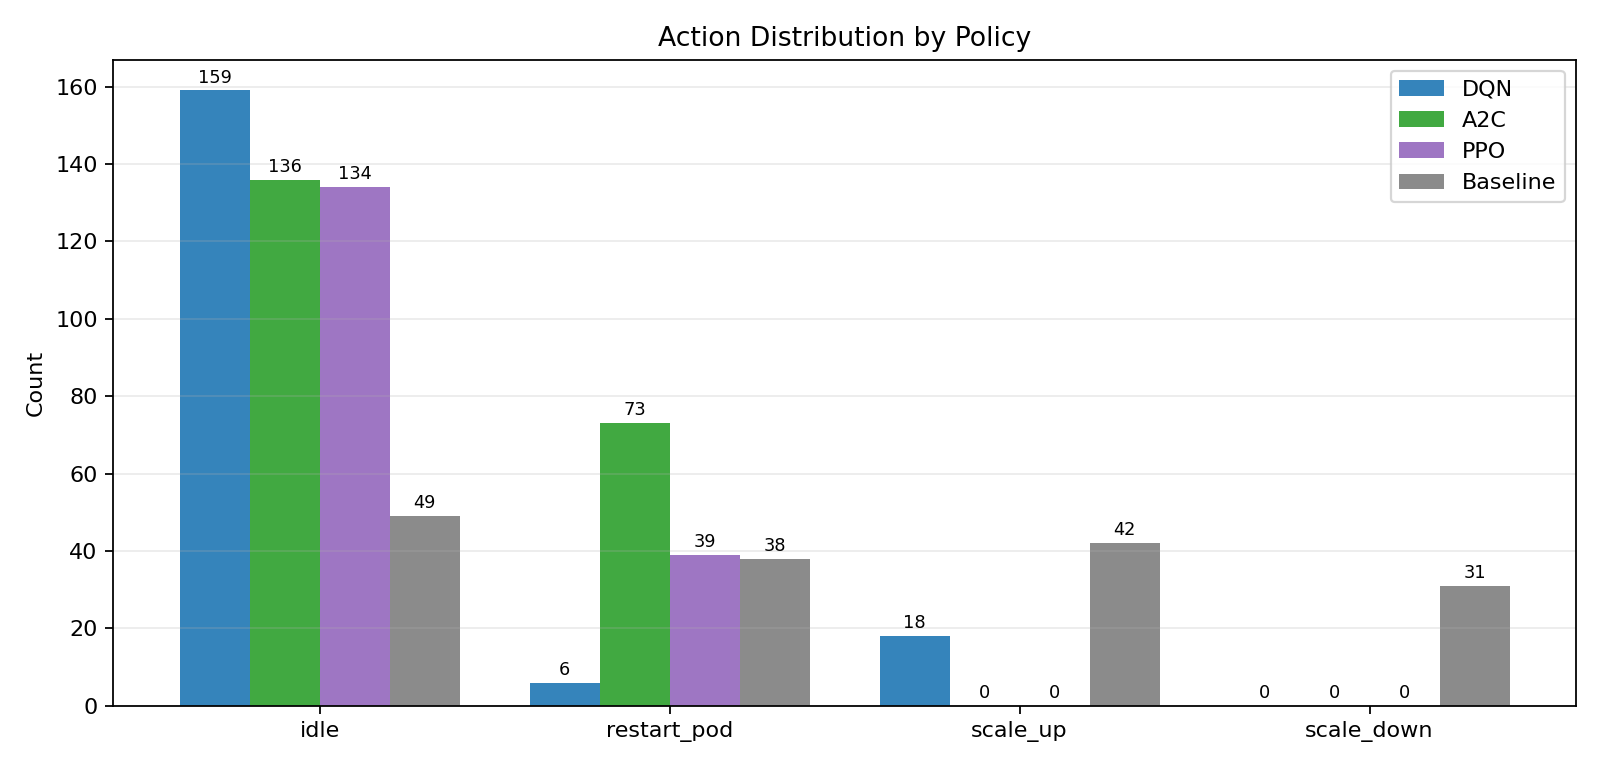
\includegraphics[width=0.92\textwidth]{graphics/chapter-6/compare/action_distribution.png}
    \captionsetup{hypcap=false}
    \captionof{figure}{Phân phối các hành động can thiệp của các thuật toán}
    \label{fig:compare-action-distribution}
\end{minipage}

\noindent Hình \ref{fig:compare-action-distribution} cho thấy sự khác biệt khá rõ trong cách ba tác nhân RL phân bổ hành động. Cả DQN, A2C và PPO đều ưu tiên mạnh hành động \texttt{idle}, với số lần lựa chọn lớn hơn nhiều so với baseline. Điều này phản ánh khả năng tránh can thiệp không cần thiết khi hệ thống đã ổn định. Ở nhóm hành động khôi phục trực tiếp, A2C sử dụng \texttt{restart\_pod} nhiều nhất (73 lần), PPO sử dụng ở mức vừa phải (39 lần), còn DQN chỉ dùng 6 lần nhưng lại thực hiện \texttt{scale\_up} 18 lần. Baseline phân bố hành động rải đều hơn, bao gồm cả \texttt{scale\_down}, cho thấy chính sách đối chứng thiếu xu hướng tập trung vào hành vi phục hồi đặc thù. Từ góc nhìn vận hành, PPO cho thấy cân bằng tốt giữa hai yêu cầu: hạn chế can thiệp thừa và vẫn giữ đủ khả năng phản ứng khi lỗi pod thực sự xảy ra.

\begin{minipage}{\textwidth}
    \centering
    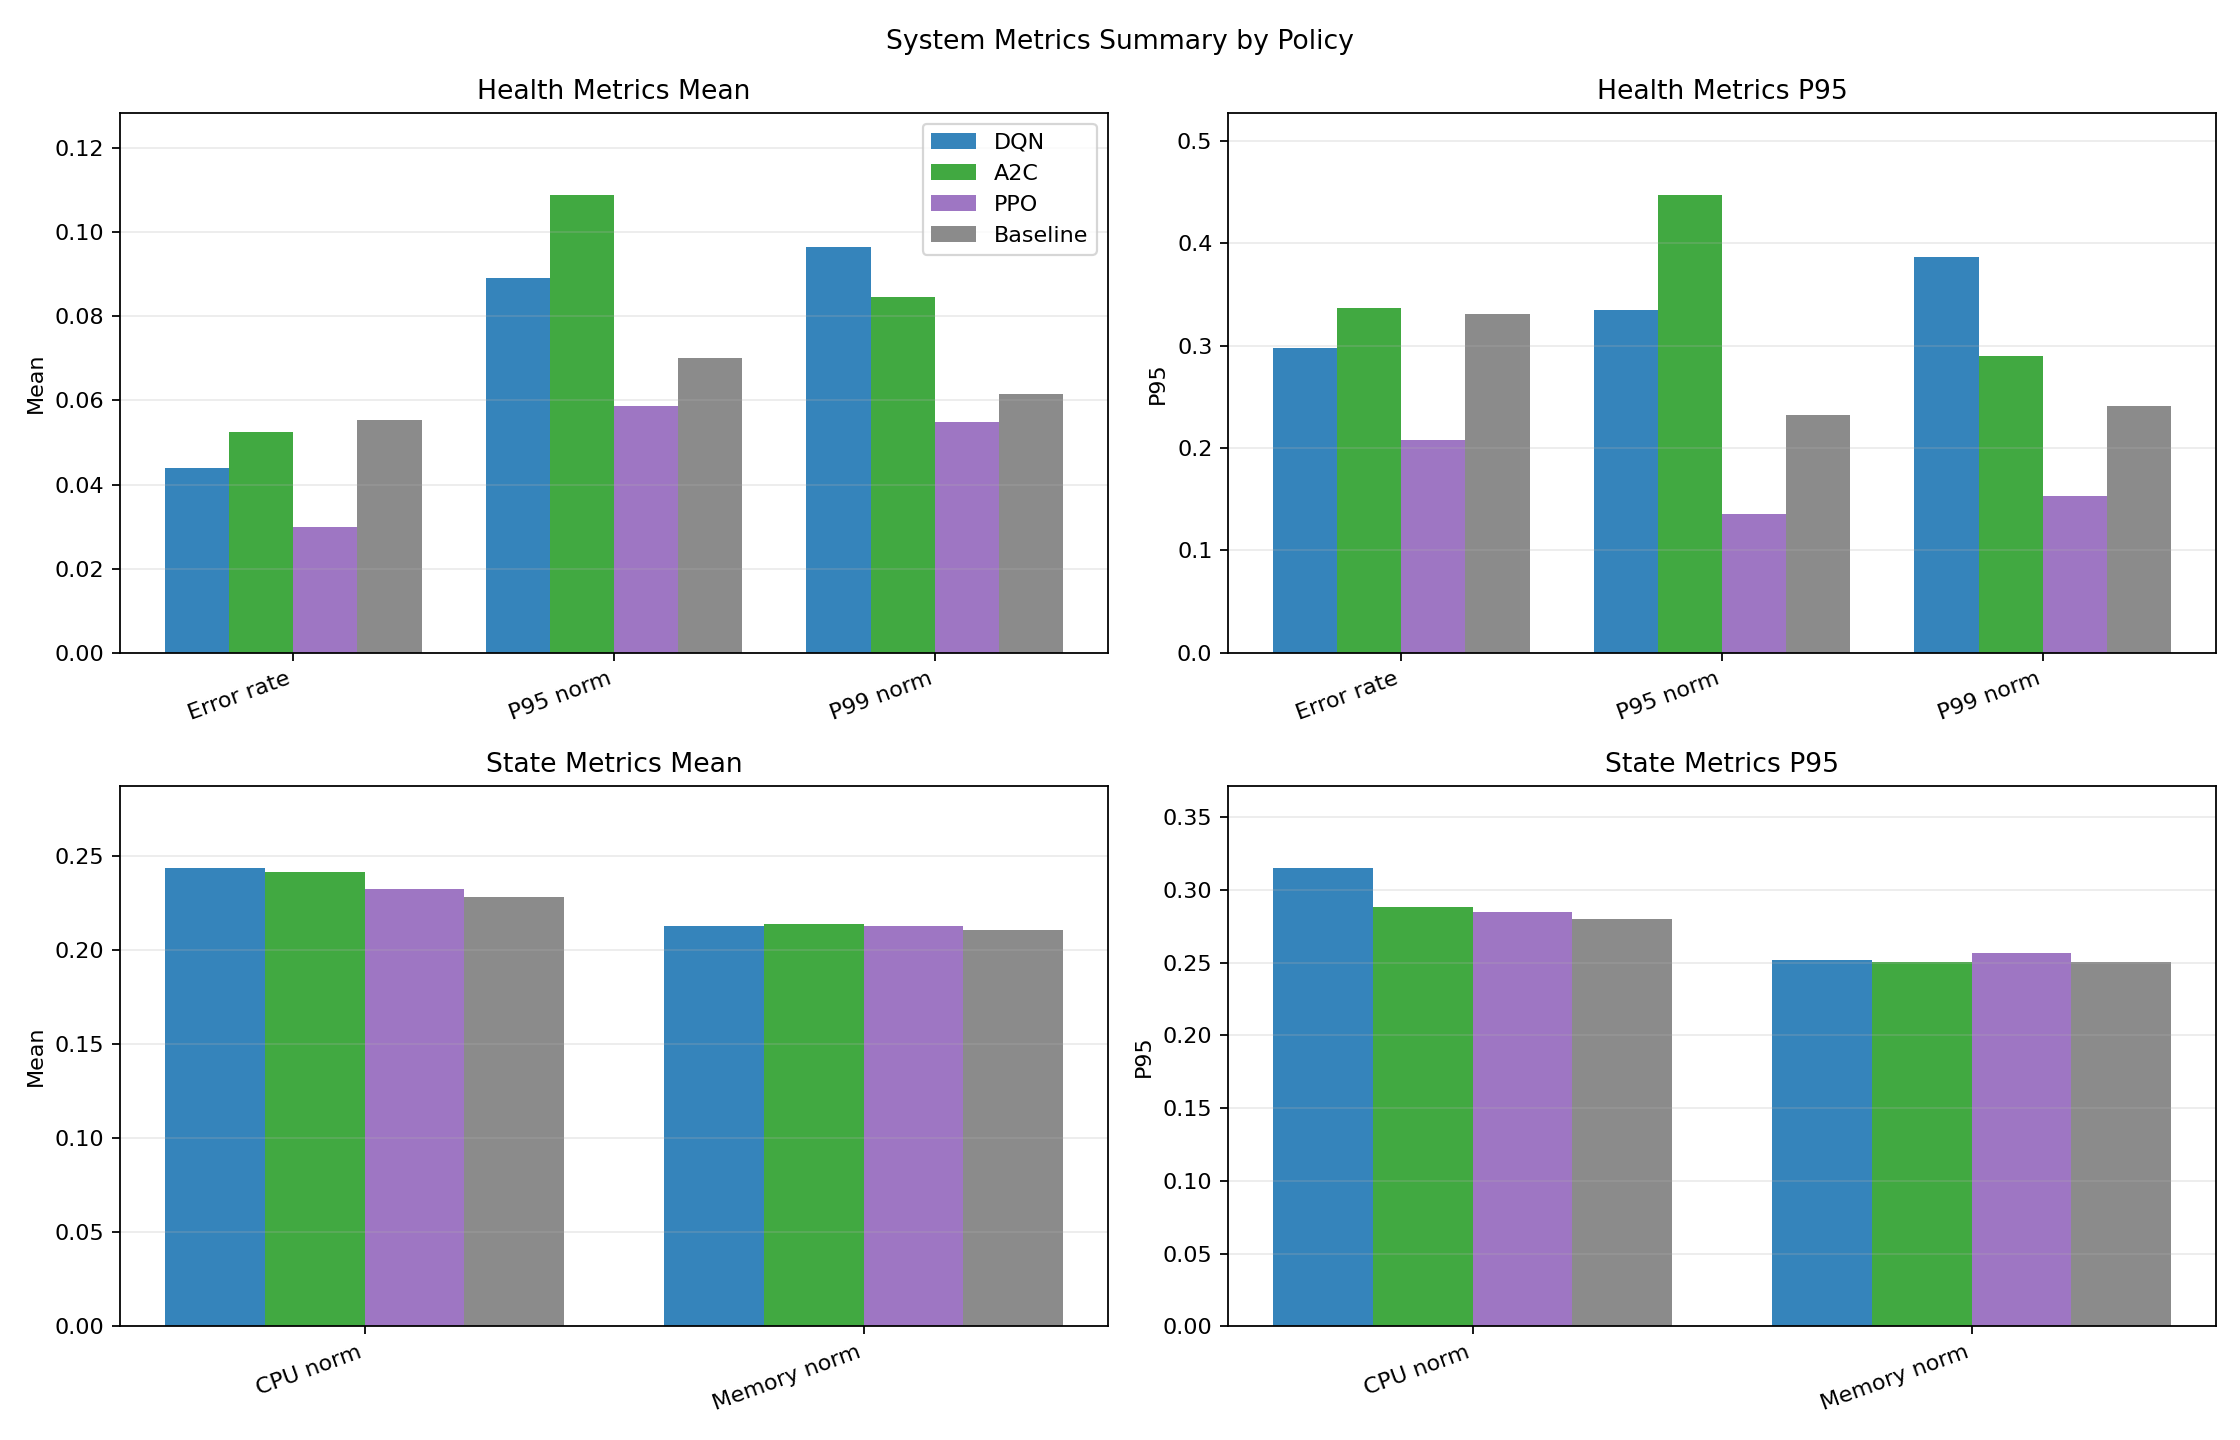
\includegraphics[width=0.95\textwidth]{graphics/chapter-6/compare/system_metrics_summary.png}
    \captionsetup{hypcap=false}
    \captionof{figure}{Tổng hợp các chỉ số hệ thống và trạng thái theo từng chính sách}
    \label{fig:compare-system-metrics}
\end{minipage}

\noindent Hình \ref{fig:compare-system-metrics} tổng hợp các chỉ số hệ thống chính dưới dạng giá trị trung bình và phân vị 95 cho bốn chính sách. Với nhóm chỉ số sức khỏe dịch vụ, PPO cho kết quả tốt nhất hoặc gần tốt nhất ở cả \textit{error rate}, \textit{p95\_norm} và \textit{p99\_norm}; đặc biệt, độ trễ ở các phân vị cao của PPO thấp hơn rõ rệt so với DQN và A2C. DQN có mức \textit{error rate} trung bình thấp hơn baseline nhưng phần đuôi độ trễ vẫn còn cao, còn A2C cho thấy \textit{p95\_norm} và \textit{p99\_norm} biến động lớn hơn. Ở nhóm chỉ số trạng thái như \textit{CPU norm} và \textit{Memory norm}, chênh lệch giữa các chính sách là không lớn, cho thấy khác biệt hiệu năng chủ yếu đến từ chất lượng ra quyết định phục hồi hơn là do một chính sách tiêu tốn tài nguyên vượt trội so với phần còn lại.

\noindent Tổng hợp bốn góc nhìn trên, có thể rút ra ba nhận xét chính. Thứ nhất, PPO là thuật toán cho kết quả tốt nhất về tổng thể khi đồng thời đạt \textit{success rate} cao nhất, phần thưởng trung bình cao nhất và các chỉ số sức khỏe dịch vụ thấp nhất. Thứ hai, DQN vẫn cho kết quả tốt hơn baseline ở cả khả năng phục hồi lẫn reward, nhưng hành vi can thiệp còn thận trọng quá mức ở \texttt{restart\_pod} và đôi khi lệch sang \texttt{scale\_up}. Thứ ba, A2C có khả năng phục hồi thành công ở mức khá nhưng độ ổn định giữa các episode chưa đồng đều bằng PPO. Vì vậy, trong phạm vi đánh giá offline của đồ án, PPO là mô hình phù hợp nhất để tiếp tục xem xét cho bước triển khai và điều khiển self-healing trên hệ thống Kubernetes.


\chapter{Kết luận và hướng phát triển}
\label{c:ketluanvahuongphattrien}
Chương này tổng kết các kết quả chính của đồ án, đồng thời nêu ra những hạn chế hiện tại và một số hướng phát triển tiếp theo.

\section{Kết luận}
\noindent Trong phạm vi đồ án, nhóm đã xây dựng được một quy trình tương đối hoàn chỉnh cho bài toán self-healing trên Kubernetes, từ hạ tầng thực nghiệm, lớp ứng dụng microservices, hệ thống giám sát, cơ chế gây lỗi cho đến mô hình học tăng cường.

\noindent Về mặt mô hình, nhóm đã biểu diễn bài toán dưới dạng MDP với trạng thái phản ánh tải, lỗi, độ trễ và ngữ cảnh pha thí nghiệm; tập hành động rời rạc gồm \texttt{idle}, \texttt{restart\_pod}, \texttt{scale\_up} và \texttt{scale\_down}; cùng hàm thưởng ưu tiên phục hồi nhanh và hạn chế vi phạm SLA.

\noindent Trên cơ sở đó, nhóm đã huấn luyện ba thuật toán DQN, A2C và PPO cho kịch bản \textit{pod failure}. Kết quả ở Chương 6 cho thấy cả ba mô hình đều tốt hơn baseline, trong đó PPO đạt kết quả nổi bật nhất về tỷ lệ thành công, phần thưởng trung bình và độ ổn định trên tập đánh giá offline.

\section{Hạn chế}
\begin{itemize}
    \item Phạm vi lỗi hiện tại chủ yếu tập trung vào kịch bản \textit{pod failure}, chưa bao phủ đầy đủ các lỗi như \textit{network delay}, \textit{node failure} hay nghẽn tài nguyên.
    \item Dữ liệu huấn luyện thực tế còn hạn chế về số lượng và độ đa dạng, nên mô hình chưa phản ánh hết các trạng thái bất thường có thể xuất hiện trong môi trường production.
    \item Quá trình huấn luyện hiện vẫn chủ yếu ở dạng offline từ artifact đã thu thập, chưa phải cơ chế học trực tiếp và liên tục trên hệ thống đang chạy.
    \item Không gian hành động còn nhỏ, nên trong một số quỹ đạo lỗi tác nhân vẫn có thể can thiệp chưa thật sự mượt hoặc lặp lại quyết định scale.
    \item Hàm thưởng hiện được thiết kế theo heuristic, phù hợp cho giai đoạn đầu nhưng chưa chắc là cấu hình tối ưu cho mọi loại dịch vụ.
\end{itemize}

\section{Hướng phát triển}
\begin{itemize}
    \item Mở rộng tập dữ liệu và kịch bản lỗi, đặc biệt với lỗi mạng, lỗi nút và các tình huống nhiều sự cố liên tiếp.
    \item Hoàn thiện guardrail an toàn để giảm hiện tượng can thiệp lặp, scale quá mức hoặc phản ứng chưa đúng ngữ cảnh.
    \item Cải tiến hàm thưởng theo hướng tinh chỉnh siêu tham số hoặc tối ưu tự động dựa trên mục tiêu vận hành.
    \item Chuyển dần sang shadow mode hoặc suy luận thời gian thực để đánh giá khả năng áp dụng của tác nhân trên cụm thật.
    \item So sánh sâu hơn giữa các thuật toán nhằm xác định mô hình phù hợp nhất cho từng loại lỗi và từng quy mô hệ thống.
\end{itemize}

\noindent Tóm lại, đồ án đã xây dựng được nền tảng thực nghiệm có tính hệ thống cho bài toán tự phục hồi Kubernetes bằng học tăng cường. Dù còn khoảng cách giữa mô hình nghiên cứu và tác nhân vận hành hoàn chỉnh, kết quả hiện tại cho thấy hướng tiếp cận RL là khả thi và có tiềm năng phát triển tiếp trong các nghiên cứu sau.


\begingroup
\setlength{\emergencystretch}{8em}
\justifying
\nocite{*}
\printbibliography[title=Tài liệu tham khảo]
\endgroup
\addcontentsline{toc}{chapter}{Tài liệu tham khảo}



\end{document}
